\documentclass[a4paper]{amsart}
\usepackage{fullpage}
\usepackage{verbatim}
\usepackage{tikz}
\usepackage{hyperref}

\definecolor{olivegreen}{cmyk}{0.64,0,0.95,0.40}
\definecolor{rawsienna}{cmyk}{0,0.72,1,0.45}

\newcommand{\GREENYELLOW}[1]{{\color{greenyellow}#1}}
\newcommand{\YELLOW}[1]{{\color{yellow}#1}}
\newcommand{\YLW}[1]{{\color{yellow}#1}}
\newcommand{\GOLDENROD}[1]{{\color{goldenrod}#1}}
\newcommand{\DANDELION}[1]{{\color{dandelion}#1}}
\newcommand{\APRICOT}[1]{{\color{apricot}#1}}
\newcommand{\PEACH}[1]{{\color{peach}#1}}
\newcommand{\MELON}[1]{{\color{melon}#1}}
\newcommand{\YELLOWORANGE}[1]{{\color{yelloworange}#1}}
\newcommand{\ORANGE}[1]{{\color{orange}#1}}
\newcommand{\BURNTORANGE}[1]{{\color{burntorange}#1}}
\newcommand{\BITTERSWEET}[1]{{\color{bittersweet}#1}}
\newcommand{\REDORANGE}[1]{{\color{redorange}#1}}
\newcommand{\MAHOGANY}[1]{{\color{mahogany}#1}}
\newcommand{\MAROON}[1]{{\color{maroon}#1}}
\newcommand{\BRICKRED}[1]{{\color{brickred}#1}}
\newcommand{\RED}[1]{{\color{red}#1}}
\newcommand{\ORANGERED}[1]{{\color{orangered}#1}}
\newcommand{\RUBINERED}[1]{{\color{rubinered}#1}}
\newcommand{\WILDSTRAWBERRY}[1]{{\color{wildstrawberry}#1}}
\newcommand{\SALMON}[1]{{\color{salmon}#1}}
\newcommand{\CARNATIONPINK}[1]{{\color{carnationpink}#1}}
\newcommand{\MAGENTA}[1]{{\color{magenta}#1}}
\newcommand{\VIOLETRED}[1]{{\color{violetred}#1}}
\newcommand{\RHODAMINE}[1]{{\color{rhodamine}#1}}
\newcommand{\MULBERRY}[1]{{\color{mulberry}#1}}
\newcommand{\REDVIOLET}[1]{{\color{redviolet}#1}}
\newcommand{\FUCHSIA}[1]{{\color{fuchsia}#1}}
\newcommand{\LAVENDER}[1]{{\color{lavender}#1}}
\newcommand{\THISTLE}[1]{{\color{thistle}#1}}
\newcommand{\ORCHID}[1]{{\color{orchid}#1}}
\newcommand{\DARKORCHID}[1]{{\color{darkorchid}#1}}
\newcommand{\PURPLE}[1]{{\color{purple}#1}}
\newcommand{\PLUM}[1]{{\color{plum}#1}}
\newcommand{\VIOLET}[1]{{\color{violet}#1}}
\newcommand{\ROYALPURPLE}[1]{{\color{royalpurple}#1}}
\newcommand{\BLUEVIOLET}[1]{{\color{blueviolet}#1}}
\newcommand{\PERIWINKLE}[1]{{\color{periwinkle}#1}}
\newcommand{\CADETBLUE}[1]{{\color{cadetblue}#1}}
\newcommand{\CORNFLOWERBLUE}[1]{{\color{cornflowerblue}#1}}
\newcommand{\MIDNIGHTBLUE}[1]{{\color{midnightblue}#1}}
\newcommand{\NAVYBLUE}[1]{{\color{navyblue}#1}}
\newcommand{\ROYALBLUE}[1]{{\color{royalblue}#1}}
\newcommand{\BLUE}[1]{{\color{blue}#1}}
\newcommand{\CERULEAN}[1]{{\color{cerulean}#1}}
\newcommand{\CYAN}[1]{{\color{cyan}#1}}
\newcommand{\PROCESSBLUE}[1]{{\color{processblue}#1}}
\newcommand{\SKYBLUE}[1]{{\color{skyblue}#1}}
\newcommand{\TURQUOISE}[1]{{\color{turquoise}#1}}
\newcommand{\TEALBLUE}[1]{{\color{tealblue}#1}}
\newcommand{\AQUAMARINE}[1]{{\color{aquamarine}#1}}
\newcommand{\BLUEGREEN}[1]{{\color{bluegreen}#1}}
\newcommand{\EMERALD}[1]{{\color{emerald}#1}}
\newcommand{\JUNGLEGREEN}[1]{{\color{junglegreen}#1}}
\newcommand{\SEAGREEN}[1]{{\color{seagreen}#1}}
\newcommand{\GREEN}[1]{{\color{green}#1}}
\newcommand{\FORESTGREEN}[1]{{\color{forestgreen}#1}}
\newcommand{\PINEGREEN}[1]{{\color{pinegreen}#1}}
\newcommand{\LIMEGREEN}[1]{{\color{limegreen}#1}}
\newcommand{\YELLOWGREEN}[1]{{\color{yellowgreen}#1}}
\newcommand{\SPRINGGREEN}[1]{{\color{springgreen}#1}}
\newcommand{\OLIVEGREEN}[1]{{\color{olivegreen}#1}}
\newcommand{\OLG}[1]{{\color{olivegreen}#1}}
\newcommand{\RAWSIENNA}[1]{{\color{rawsienna}#1}}
\newcommand{\SEPIA}[1]{{\color{sepia}#1}}
\newcommand{\BROWN}[1]{{\color{brown}#1}}
\newcommand{\TAN}[1]{{\color{tan}#1}}
\newcommand{\GRAY}[1]{{\color{gray}#1}}
\newcommand{\LGRAY}[1]{{\color{gray!40}#1}}
\newcommand{\WHITE}[1]{{\color{white}#1}}
\newcommand{\BLACK}[1]{{\color{black}#1}}


\newcommand{\bbm}       {\left[\begin{matrix}}
\newcommand{\ebm}       {\end{matrix}\right]}
\newcommand{\bsm}       {\left[\begin{smallmatrix}}
\newcommand{\esm}       {\end{smallmatrix}\right]}
\newcommand{\bpm}       {\begin{pmatrix}}
\newcommand{\epm}       {\end{pmatrix}}
\newcommand{\bcf}[2]{\left(\begin{array}{c}{#1}\\{#2}\end{array}\right)}


\newcommand{\csch}     {\operatorname{csch}}
\newcommand{\sech}     {\operatorname{sech}}
\newcommand{\arcsinh}  {\operatorname{arcsinh}}
\newcommand{\arccosh}  {\operatorname{arccosh}}
\newcommand{\arctanh}  {\operatorname{arctanh}}

\newcommand{\range}     {\operatorname{range}}
\newcommand{\trans}     {\operatorname{trans}}
\newcommand{\trc}       {\operatorname{trace}}
\newcommand{\adj}       {\operatorname{adj}}

\newcommand{\dv}        {\operatorname{div}}
\newcommand{\grad}      {\operatorname{grad}}
\newcommand{\curl}      {\operatorname{curl}}

\newcommand{\tint}{\textstyle\int}
\newcommand{\tm}{\times}
\newcommand{\sse}{\subseteq}
\newcommand{\st}{\;|\;}
\newcommand{\sm}{\setminus}
\newcommand{\iffa}      {\Leftrightarrow}
\newcommand{\xra}{\xrightarrow}

\newcommand{\half}{\tfrac{1}{2}}

\renewcommand{\:}{\colon}

\newcommand{\N}         {{\mathbb{N}}}
\newcommand{\Z}         {{\mathbb{Z}}}
\newcommand{\Q}         {{\mathbb{Q}}}
\newcommand{\R}         {{\mathbb{R}}}
\newcommand{\C}         {{\mathbb{C}}}

\newcommand{\va}        {\mathbf{a}}
\newcommand{\vb}        {\mathbf{b}}
\newcommand{\vc}        {\mathbf{c}}
\newcommand{\vd}        {\mathbf{d}}
\newcommand{\ve}        {\mathbf{e}}
\newcommand{\vf}        {\mathbf{f}}
\newcommand{\vg}        {\mathbf{g}}
\newcommand{\vh}        {\mathbf{h}}
\newcommand{\vi}        {\mathbf{i}}
\newcommand{\vj}        {\mathbf{j}}
\newcommand{\vk}        {\mathbf{k}}
\newcommand{\vl}        {\mathbf{l}}
\newcommand{\vm}        {\mathbf{m}}
\newcommand{\vn}        {\mathbf{n}}
\newcommand{\vo}        {\mathbf{o}}
\newcommand{\vp}        {\mathbf{p}}
\newcommand{\vq}        {\mathbf{q}}
\newcommand{\vr}        {\mathbf{r}}
\newcommand{\vs}        {\mathbf{s}}
\newcommand{\vt}        {\mathbf{t}}
\newcommand{\vu}        {\mathbf{u}}
\newcommand{\vv}        {\mathbf{v}}
\newcommand{\vw}        {\mathbf{w}}
\newcommand{\vx}        {\mathbf{x}}
\newcommand{\vy}        {\mathbf{y}}
\newcommand{\vz}        {\mathbf{z}}

\newcommand{\hva}       {\widehat{\mathbf{a}}}
\newcommand{\hvb}       {\widehat{\mathbf{b}}}
\newcommand{\hvc}       {\widehat{\mathbf{c}}}
\newcommand{\hvd}       {\widehat{\mathbf{d}}}
\newcommand{\hve}       {\widehat{\mathbf{e}}}
\newcommand{\hvf}       {\widehat{\mathbf{f}}}
\newcommand{\hvg}       {\widehat{\mathbf{g}}}
\newcommand{\hvh}       {\widehat{\mathbf{h}}}
\newcommand{\hvi}       {\widehat{\mathbf{i}}}
\newcommand{\hvj}       {\widehat{\mathbf{j}}}
\newcommand{\hvk}       {\widehat{\mathbf{k}}}
\newcommand{\hvl}       {\widehat{\mathbf{l}}}
\newcommand{\hvm}       {\widehat{\mathbf{m}}}
\newcommand{\hvn}       {\widehat{\mathbf{n}}}
\newcommand{\hvo}       {\widehat{\mathbf{o}}}
\newcommand{\hvp}       {\widehat{\mathbf{p}}}
\newcommand{\hvq}       {\widehat{\mathbf{q}}}
\newcommand{\hvr}       {\widehat{\mathbf{r}}}
\newcommand{\hvs}       {\widehat{\mathbf{s}}}
\newcommand{\hvt}       {\widehat{\mathbf{t}}}
\newcommand{\hvu}       {\widehat{\mathbf{u}}}
\newcommand{\hvv}       {\widehat{\mathbf{v}}}
\newcommand{\hvw}       {\widehat{\mathbf{w}}}
\newcommand{\hvx}       {\widehat{\mathbf{x}}}
\newcommand{\hvy}       {\widehat{\mathbf{y}}}
\newcommand{\hvz}       {\widehat{\mathbf{z}}}

\newcommand{\vA}        {\mathbf{A}}
\newcommand{\vB}        {\mathbf{B}}
\newcommand{\vC}        {\mathbf{C}}
\newcommand{\vD}        {\mathbf{D}}
\newcommand{\vE}        {\mathbf{E}}
\newcommand{\vF}        {\mathbf{F}}
\newcommand{\vG}        {\mathbf{G}}
\newcommand{\vH}        {\mathbf{H}}
\newcommand{\vI}        {\mathbf{I}}
\newcommand{\vJ}        {\mathbf{J}}
\newcommand{\vK}        {\mathbf{K}}
\newcommand{\vL}        {\mathbf{L}}
\newcommand{\vM}        {\mathbf{M}}
\newcommand{\vN}        {\mathbf{N}}
\newcommand{\vO}        {\mathbf{O}}
\newcommand{\vP}        {\mathbf{P}}
\newcommand{\vQ}        {\mathbf{Q}}
\newcommand{\vR}        {\mathbf{R}}
\newcommand{\vS}        {\mathbf{S}}
\newcommand{\vT}        {\mathbf{T}}
\newcommand{\vU}        {\mathbf{U}}
\newcommand{\vV}        {\mathbf{V}}
\newcommand{\vW}        {\mathbf{W}}
\newcommand{\vX}        {\mathbf{X}}
\newcommand{\vY}        {\mathbf{Y}}
\newcommand{\vZ}        {\mathbf{Z}}

\newcommand{\ddx}       {\frac{\partial}{\partial x}}
\newcommand{\ddy}       {\frac{\partial}{\partial y}}
\newcommand{\ddz}       {\frac{\partial}{\partial z}}
\newcommand{\ddr}       {\frac{\partial}{\partial r}}
\newcommand{\ddt}       {\frac{\partial}{\partial\theta}}
\newcommand{\ddp}       {\frac{\partial}{\partial\phi}}

\newcommand{\al}        {\alpha}
\newcommand{\bt}        {\beta} 
\newcommand{\gm}        {\gamma}
\newcommand{\dl}        {\delta}
\newcommand{\ep}        {\epsilon}
\newcommand{\zt}        {\zeta}
\newcommand{\et}        {\eta}
\newcommand{\tht}       {\theta}
\newcommand{\io}        {\iota}
\newcommand{\kp}        {\kappa}
\newcommand{\lm}        {\lambda}
\newcommand{\ph}        {\phi}
\newcommand{\ch}        {\chi}
\newcommand{\ps}        {\psi}
\newcommand{\rh}        {\rho}
\newcommand{\sg}        {\sigma}
\newcommand{\om}        {\omega}

%%% Note: remember the macros \ddt and \ddp as well
\newcommand{\zen}       {\phi}   % zenith angle
\newcommand{\azi}       {\theta} % azimuth angle

\newcommand{\CH}[1]     {\left[\vphantom{\int}#1\right]}
\newcommand{\ov}        {\overline}

\renewcommand{\ss}      {\scriptstyle}

\newcommand{\EMPH}[1]{\emph{\RED{#1}}}
\newcommand{\DEFN}[1]{\emph{\PURPLE{#1}}}
\newcommand{\VEC}[1]    {\mathbf{#1}}

\newcommand{\ghost}{{\tiny $\color[rgb]{1,1,1}.$}}

\newcommand{\uc}{\uncover}

\newcommand{\bbox}[1]{
\[ \mbox{\begin{tikzpicture}%
   \draw(0,0) node[draw,thick,olivegreen,rectangle] {\color{black} #1};%
  \end{tikzpicture}} \]
}

\newcommand{\cbox}[1]{
\begin{center}\begin{tikzpicture}%
   \draw(0,0) node[draw,thick,olivegreen,rectangle] {\color{black} #1};%
\end{tikzpicture}\end{center}
}

% Foreground and background for tikz.
% This default is for screen mode.
\newcommand{\fg}{white}
\newcommand{\bg}{black}
\newcommand{\mg}{gray}

\makeatletter

% An environment for a solution that is included inline.
\newenvironment{SolutionInline}{{\noindent \bf Solution:}}{}

% An environment that makes a solution completely invisible.
\newenvironment{SolutionHidden}
 {\@bsphack
  \let\do\@makeother\dospecials\catcode`\^^M\active
  \def\verbatim@processline{}%
 \verbatim@start}%
{\@esphack\par\vspace{2ex}}

%\newenvironment{solution}{\SolutionInline}{\endSolutionInline}
\newenvironment{solution}{\SolutionHidden}{\endSolutionHidden}

\makeatother

\theoremstyle{definition}
\newtheorem{exercise}{Exercise}



\title{MAS243 Problems}

\def\SOLS{1}
\ifx\SOLS\undefined\else
\renewenvironment{solution}{\SolutionInline}{\endSolutionInline}
\fi

\begin{document}

\maketitle

\section*{Week 1 --- Optimisation}

\begin{exercise}
 Find the maximum and minimum values of the function
 $f(x)=x^3-9x^2+15x+35$ with $0\leq x\leq 8$.
\end{exercise}
\begin{solution}
 We have 
 \[ f'(x)=3x^2-18x+15=3(x^2-6x+5)=3(x-1)(x-5), \]
 so the critical points are $x=1$ and $x=5$.  We need to check the
 values of $f(x)$ at the endpoints and the critical points:
 \begin{align*}
  f(0) &= 35 \\
  f(1) &= 42 \\
  f(5) &= 125-9\tm 25+15\tm 5+35 = 10 \\
  f(8) &= 512-9\tm 64+15\tm 8+35 = 91.
 \end{align*}
 Thus, the smallest value is $10$ (at the critical point $x=5$) and
 the largest value is $91$ (at the endpoint $x=8$).
 \begin{center}
  \begin{tikzpicture}[scale=1]
   \def\ff{(35+(15+(-9+\x)*\x)*\x)/24}
   \draw[->] (-0.1,0) -- (8.1,0);
   \draw[->] (0,0) -- (0,4.1);
   \draw[red,domain=0:8,samples=300,smooth,variable=\x] plot({\x},{\ff});
   \foreach \x in {0,1,5,8} {
    \draw[blue]  (\x,0) -- (\x,{\ff});
    \fill[black] (\x,0) circle(0.04);
    \fill[black] (\x,{\ff}) circle(0.04);
   }
   \draw (0,-0.1) node[anchor=north]{$0$};
   \draw (1,-0.1) node[anchor=north]{$1$};
   \draw (5,-0.1) node[anchor=north]{$5$};
   \draw (8,-0.1) node[anchor=north]{$8$};
  \end{tikzpicture}
 \end{center}
 Note that this is very similar to Example~(d) on pages 3-4 of the 
 \href{http://shef.ac.uk/nps/courses/MAS243/MAS243.pdf}{course notes}.
\end{solution}

\begin{exercise}
 Find and classify the critical points of the function
 $f(x)=\cos(x)-\cos^3(x)/3$.  What is the unusual feature of this
 example? 
\end{exercise}
\begin{solution}
 The derivatives are 
 \begin{align*}
  f'(x) &= -\sin(x)+\cos^2(x)\sin(x) 
         = -\sin(x)(1-\cos^2(x)) 
         = -\sin(x)\sin^2(x) \\
        &= -\sin^3(x) \\
  f''(x) &= -3\sin^2(x)\cos(x).
 \end{align*}
 The critical points are the points $x$ where $\sin^3(x)=0$ or
 equivalently $\sin(x)=0$ or $x=n\pi$ for integers $n$.  For such
 points we have $f''(x)=3\sin^2(x)\cos(x)=0$, so the second derivative
 does not help us to decide whether we have a local maximum or a local
 minimum (this is the unusual feature).  However, when $x$ lies
 between $2m\pi$ and $(2m+1)\pi$ we have $\sin(x)>0$ so
 $f'(x)=-\sin^3(x)<0$ so $f(x)$ is decreasing.  On the other hand,
 when $x$ lies between $(2m+1)\pi$ and $(2m+2)\pi$ we have $\sin(x)<0$
 so $f'(x)=-\sin^3(x)>0$ so $f(x)$ is increasing.  It follows that the
 points $x=2m\pi$ are maxima and the points $x=(2m+1)\pi$ are minima,
 with
 \begin{align*}
  f(2m\pi) &= \cos(2m\pi) - \cos^3(2m\pi)/3
            = 1 - 1/3 = 2/3 \\
  f((2m+1)\pi) &= \cos((2m+1)\pi) - \cos^3((2m+1)\pi)/3
            = -1 + 1/3 = -2/3.
 \end{align*}
 If you did not notice the trick of rewriting $f'(x)$ as $-\sin^3(x)$,
 you would get 
 \begin{align*}
  f'(x) &= -\sin(x)(1-\cos^2(x)) \\
  f''(x) &= -\cos(x)-2\cos(x)\sin^2(x)+cos^3(x).
 \end{align*}
 You would then say that there are critical points where $\sin(x)=0$
 or $\cos(x)=\pm 1$, but that again gives $x=n\pi$.  After remembering
 that $\cos(n\pi)=(-1)^n$ you would then get $f''(n\pi)=0$ again.
 This is less tidy but essentially the same.

 In the following picture, the red graph is $f(x)$ and the blue graph
 is $f'(x)$.
 \begin{center}
  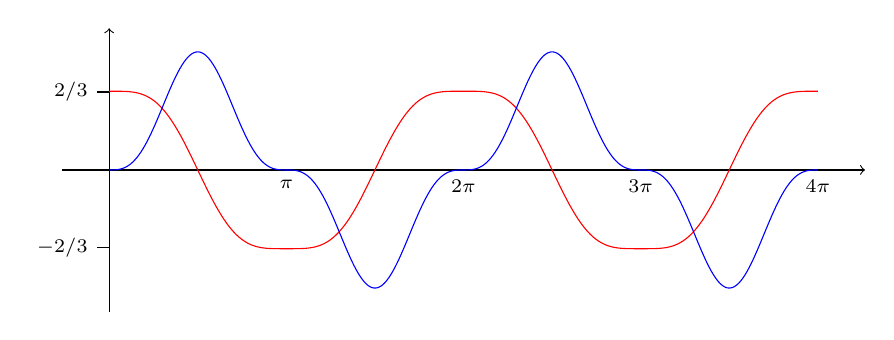
\begin{tikzpicture}[scale=1.5]
   \draw[->] (-0.4,0) -- (6.4,0);
   \draw[->] (0,-1.2) -- (0,1.2);
   \draw (-0.1, 0.66) -- (0, 0.66);
   \draw (-0.1,-0.66) -- (0,-0.66);
   \draw[red,domain=0:720,samples=400,smooth,variable=\x]
    plot({\x/120},{cos(\x)-cos(\x)^3/3});
   \draw[blue,domain=0:720,samples=400,smooth,variable=\x]
    plot({\x/120},{sin(\x)^3});
   \draw (1.5,0) node[anchor=north] {$\ss \pi$};
   \draw (3.0,0) node[anchor=north] {$\ss 2\pi$};
   \draw (4.5,0) node[anchor=north] {$\ss 3\pi$};
   \draw (6.0,0) node[anchor=north] {$\ss 4\pi$};
   \draw (-0.1, 0.66) node[anchor=east] {$\ss 2/3$};
   \draw (-0.1,-0.66) node[anchor=east] {$\ss -2/3$};
  \end{tikzpicture}
 \end{center}
 You should see that the graph of $f(x)$ is unusually flat at the top
 and the bottom, much flatter than the graph of $\sin(x)$ or
 $\cos(x)$.  This is a reflection of the fact that $f''(x)=0$ at the
 critical points.
\end{solution}

\begin{exercise}
 Show that $\sqrt{2}\sin(x-\pi/4)=\sin(x)-\cos(x)$.  Using this, find
 the maximum value of $e^{-x}\sin(x)$ for $x\geq 0$.
\end{exercise}
\begin{solution}
 We start with the standard addition formula
 \[ \sin(x+y) = \sin(x)\cos(y) + \cos(x)\sin(y). \]
 Take $y=-\pi/4$, recalling that
 $\sin(-\pi/4)=-\sin(\pi/4)=-1/\sqrt{2}$ and
 $\cos(-\pi/4)=\cos(\pi/4)=1/\sqrt{2}$.  This gives
 $\sin(x-\pi/4)=(\sin(x)-\cos(x))/\sqrt{2}$, so
 $\sqrt{2}\sin(x-\pi/4)=\sin(x)-\cos(x)$ as claimed.

 Now consider the function $f(x)=e^{-x}\sin(x)$.  This has
 \[ f'(x) = -e^{-x}\sin(x) + e^{-x}\cos(x) = 
     e^{-x}(\cos(x)-\sin(x)) = -\sqrt{2} e^{-x}\sin(x-\pi/4).
 \]
 For a critical point we must have $f'(x)=0$.  As $e^{-x}$ is never
 zero, this gives $\sin(x-\pi/4)=0$, so $x-\pi/4$ must be a multiple
 of $\pi$, so $x=n\pi+\pi/4$ for some integer $n$.  We are only
 interested in the case $x\geq 0$, so we must have $n\geq 0$.  Note
 also that $\sin(\pi+x)=-\sin(x)$, so
 \[ \sin(n\pi+\pi/4)=(-1)^n\sin(\pi/4)=(-1)^n/\sqrt{2}. \]
 Using this we get 
 \[ f(n\pi+\pi/4) = (-1)^n e^{-n\pi}e^{-\pi/4}/\sqrt{2}. \]
 These numbers alternate in sign, and the absolute values get smaller
 as $n$ increases.  It follows that we have the largest value when
 $n=0$, namely $f(\pi/2)=e^{-\pi/4}/\sqrt{2}\simeq 0.32$.  We also
 need to check what happens at the endpoints but $f(0)=0$ and $f(x)$
 decays rapidly to zero as $x\to\infty$, so our conclusionis
 unaffected.  The picture is like this:
 \begin{center}
  \begin{tikzpicture}[scale=2]
   \def\ff{6*sin(57.3*\x)/exp(\x)}
   \draw[->] (-0.1,0) -- (5,0);
   \draw[->] (0,0) -- (0,2.1);
   \draw[red,domain=0:5,samples=300,smooth,variable=\x] plot({\x},{\ff});
   \draw[blue] (0.785,0) -- (0.785,1.934);
   \fill[black] (0.785,0) circle(0.03);
   \fill[black] (1.571,0) circle(0.03);
   \fill[black] (0.785,1.934) circle(0.03);
   \draw (5.2,0) node{$x$};
   \draw (0.785,-0.1) node[anchor=north]{$\frac{\pi}{4}$};
   \draw (1.571,-0.1) node[anchor=north]{$\frac{\pi}{2}$};
  \end{tikzpicture}
 \end{center}
\end{solution}

\begin{exercise}
 For the following functions, calculate the partial derivatives $f_x$ and $f_y$, 
 and verify that $f_{xy}=f_{yx}$.
 \begin{itemize}
  \item[(a)] $f(x,y)=x^3+3x^2y+xy^2+4y^3$
  \item[(b)] $f(x,y)=xy^2\ln(x^2+y^2)$.
 \end{itemize}
\end{exercise}
\begin{solution}
 \begin{itemize}
  \item[(a)]
   \begin{align*}
    f_x(x,y) &= 3x^{2} + 6xy + y^{2} & f_y(x,y) &= 3x^{2} + 2xy + 12 y^{2} \\
    f_{xy}(x,y) &= 6x+2y & f_{yx}(x,y) &= 6x+2y. 
   \end{align*}
  \item[(b)] 
   First note that the online test asked you to enter $f_x$ rather than
   $f_{xy}$ here, in an attempt to save you some pain.  Unfortunately many
   students misread the question.

   To calculate the relevant derivatives, the chain rule gives 
   \[ \frac{\partial}{\partial x}\ln(x^2+y^2) = \frac{2x}{x^2+y^2}. \]
   To explain this in more detail, put $u=x^2+y^2$ and $v=\ln(u)$.  We then have 
   $dv/du=1/u=1/(x^2+y^2)$ and $\partial u/\partial x=2x$ so the chain rule gives 
   \[ \frac{\partial v}{\partial x} =
       \frac{dv}{du} \; \frac{\partial u}{\partial x} = 
        \frac{2x}{x^2+y^2}
   \]
   as claimed.  Similarly, we have $\partial v/\partial
   y=2y/(x^2+y^2)$.  Using this together with the product rule we get 
   \begin{align*}
    f_x(x,y)    &= y^2\ln(x^2+y^2) + 2x^2y^2/(x^2+y^2) \\
    f_y(x,y)    &= 2xy\ln(x^2+y^2) + 2xy^3/(x^2+y^2).
   \end{align*}

   We now want to calculate $f_{xy}(x,y)$.  We can differentiate
   $y^2\ln(x^2+y^2)$ by the same method that we just used for
   $xy^2\ln(x^2+y^2)$.  For the second term we use the quotient rule
   $(u/v)_x=(u_xv-uv_x)/v^2$ (with $u=2x^2y^2$ and $v=x^2+y^2$).  This
   gives 
   \[ \frac{\partial}{\partial y}\left(\frac{2x^2y^2}{x^2+y^2}\right)
       = \frac{4x^2y(x^2+y^2)-2x^2y^2.2y}{(x^2+y^2)^2}
       = \frac{4x^4y}{(x^2+y^2)^2},
   \]
   so 
   \begin{align*}
    f_{xy}(x,y) &= 2y\ln(x^2+y^2) + \frac{y^2.2y}{x^2+y^2} + 
                     \frac{4x^4y}{(x^2+y^2)^2} \\
     &= 2y\ln(x^2+y^2) + \frac{2y^3(x^2+y^2)+4x^4y}{(x^2+y^2)^2} 
      = 2y\ln(x^2+y^2) + \frac{4x^4y + 2x^2y^3 + 2y^5}{(x^2+y^2)^2}. 
   \end{align*}
   In the same way, we have
   \[ \frac{\partial}{\partial x}\left(\frac{2xy^3}{x^2+y^2}\right)
       = \frac{2y^3(x^2+y^2)-2xy^3.2x}{(x^2+y^2)^2}
       = \frac{2y^5-2x^2y^3}{(x^2+y^2)^2},
   \]
   so 
   \begin{align*}
    f_{yx}(x,y) &= 2y\ln(x^2+y^2) + \frac{2xy.2x}{x^2+y^2} +
                    \frac{2y^5-2x^2y^3}{(x^2+y^2)^2} \\
     &= 2y\ln(x^2+y^2) + \frac{4x^2y(x^2+y^2)+2y^5-2x^2y^3}{(x^2+y^2)^2}
      = 2y\ln(x^2+y^2) + \frac{4x^4y + 2x^2y^3 + 2y^5}{(x^2+y^2)^2}.
   \end{align*}
   This is the same as $f_{xy}(x,y)$, as expected.
 \end{itemize}
\end{solution}

\begin{exercise}
 Suppose we have a function $f(x,y)$ of two variables.  We say that
 $f$ is biharmonic if it satisfies the equation
 \[ f_{xxxx} + 2 f_{xxyy} + f_{yyyy} = 0. \]
 (This comes up in the theory of small elastic deformations of nearly
 rigid bodies.) Show that the function $f(x,y)=xy^2(x^2-y^2)$ is
 biharmonic but the function $g(x,y)=e^{x+y}$ is not.
\end{exercise}
\begin{solution}
 We have $f=x^3y^2-xy^4$ so
 \begin{align*}
  f_x &= 3x^2y^2 - y^4 &
  f_{xx} &= 6xy^2 & 
  f_{xxx} &= 6y^2 & 
  f_{xxxx} &= 0 \\
  f_y &= 2x^3y - 4xy^3 &
  f_{yy} &= 2x^3-12xy^2 & 
  f_{yyy} &= -24xy & 
  f_{yyyy} &= -24x \\
  f_{xxy} &= 12xy & 
  f_{xxyy} &= 12x
 \end{align*}
 so 
 \[ f_{xxxx} + 2 f_{xxyy} + f_{yyyy} = 0 + 2\tm 12x - 24x = 0. \]
 This means that $f$ is biharmonic.

 On the other hand we have $g_x=e^{x+y}=g$ and $g_y=e^{x+y}=g$, and it
 follows in turn that $g_{xx}=g$ and $g_{xxx}=g$ and $g_{xxxx}=g$.
 Similarly we have $g_{xxyy}=g$ and $g_{yyyy}=g$ so 
 \[ g_{xxxx} + 2 g_{xxyy} + g_{yyyy} = 4g = 4e^{x+y} \neq 0, \]
 so $g$ is not biharmonic.
\end{solution}

\begin{exercise}
 Show that the function $f(x,t)=t^{-1/2}e^{-x^2/t}$ satisfies the
 equation $4f_t=f_{xx}$.  (This is relevant to the equations of heat
 flow, and also to the pricing of financial derivatives.)
\end{exercise}
\begin{solution}
 To find $f_t$ we break $f$ into pieces, putting $u=t^{-1/2}$ and
 $v=e^{-x^2/t}$ and $w=-x^2/t$.  It is straightforward that
 \begin{align*}
  u_t &= \frac{\partial u}{\partial t}
       = -\tfrac{1}{2}t^{-3/2} \\
  w_t &= \frac{\partial w}{\partial t} 
       = -x^2 \frac{\partial}{\partial t}(t^{-1}) 
       = -x^2 \tm (-t^{-2}) = x^2t^{-2}.
 \end{align*}
 Next, we have $v=e^w$ so the chain rule gives
 \begin{align*}
  v_t &= \frac{\partial v}{\partial t} 
       = \frac{dv}{dw} \; \frac{\partial w}{\partial t} 
       = e^w x^2 t^{-2}
       = x^2 t^{-2} e^{-x^2/t}.
 \end{align*}
 We now note that $f=uv$ and use the product rule:
 \begin{align*}
  f_t &= (uv)_t = u_t v + u\,v_t \\
      &= -\tfrac{1}{2} t^{-3/2} e^{-x^2/t} 
         + t^{-1/2} x^2 t^{-2} e^{-x^2/t} \\
      &= (-t^{-3/2}/2 + x^2t^{-5/2}) e^{-x^2/t}.
 \end{align*}
 On the other hand, using the chain rule and te product rule we have
 \begin{align*}
  f_x &= (-2x/t)t^{-1/2} e^{-x^2/t} 
       = -2x t^{-3/2} e^{-x^2/t} \\
  f_{xx} &= -2t^{-3/2} e^{-x^2/t} + 
              (2x/t) 2x t^{-3/2} e^{-x^2/t}
          = (-2t^{-3/2} + 4x^2t^{-5/2}) e^{-x^2/t}. 
 \end{align*}
 It is now clear that $4f_t=f_{xx}$ as claimed.
\end{solution}

\begin{exercise}
 Find the critical points of the function
 $f(x,y)=(x+y+2)e^{-(x^2+y^2)/2}$.
\end{exercise}
\begin{solution}
 The derivatives are
 \begin{align*}
  f_x &= e^{-(x^2+y^2)/2} -x(x+y+2)e^{-(x^2+y^2)/2}
       = (1-x(x+y+2)) e^{-(x^2+y^2)/2} \\
  f_y &= e^{-(x^2+y^2)/2} -y(x+y+2)e^{-(x^2+y^2)/2}
       = (1-y(x+y+2)) e^{-(x^2+y^2)/2}.
 \end{align*}
 These must both be zero.  As exponentials are never zero, this
 implies that $1-x(x+y+2)=1-y(x+y+2)=0$.  This gives $x=1/(x+y+2)$ and
 also $y=1/(x+y+2)$ so $y=x$.  Putting $y=x$ in the equation
 $1-x(x+y+2)=0$ gives $1-2x^2-2x=0$ so $x^2+x-1/2=0$ which gives
 $x=(-1\pm\sqrt{3})/2$.  It follows that the critical points are
 $(x,y)=((-1+\sqrt{3})/2,(-1+\sqrt{3})/2)\simeq(0.366,0.366)$ and 
 $(x,y)=((-1-\sqrt{3})/2,(-1-\sqrt{3})/2)\simeq(-1.366,-1.366)$.
\end{solution}

\begin{exercise}
 Let $\phi$ be a constant.  The function 
 \[ f(x,y)=(x^2+y^2)^2-x\cos(\phi)/2-y\sin(\phi)/2 \]
 has only one critical point.  Find it.
\end{exercise}
\begin{solution}
 The derivatives are
 \begin{align*}
  f_x &= 2(x^2+y^2)\tm 2x - \cos(\phi)/2 \\
  f_y &= 2(x^2+y^2)\tm 2y - \sin(\phi)/2.
 \end{align*}
 These must both be zero, which means that
 \begin{align*}
  \cos(\phi) &= 8x(x^2+y^2) \\
  \sin(\phi) &= 8y(x^2+y^2).
 \end{align*}
 Squaring these equations and adding them together, we get
 \begin{align*}
  1 &= \cos^2(\phi)+\sin^2(\phi) 
     = 64x^2(x^2+y^2)^2 + 64y^2(x^2+y^2)^2 \\
    &= 64 (x^2+y^2)(x^2+y^2)^2 = 64(x^2+y^2)^3.
 \end{align*}
 This gives $x^2+y^2=(1/64)^{1/3}=1/4$.  Feeding this back into the
 equation $\cos(\phi)=8x(x^2+y^2)$ gives $\cos(\phi)=2x$ and so
 $x=\cos(\phi)/2$.  Similarly, the equation $\sin(\phi)=8y(x^2+y^2)$
 gives $\sin(\phi)=2y$ and so $y=\sin(\phi)/2$.  Thus, the unique
 critical point is $(x,y)=(\cos(\phi)/2,\sin(\phi)/2)$.
\end{solution}

\section*{Week 2 --- Constrained optimisation}

\begin{exercise}
 Show that the function $u=x^3+x^2y-y^2-2x^2$ has critical points at
 $(0,0)$, $(1,1/2)$ and $(-4,8)$, and determine their nature.
\end{exercise}
\begin{solution}
 The partial derivatives are
 \begin{align*}
   u_x &= 3x^2+2xy-4x &&& u_y &= x^2-2y \\
   u_{xx} &= 6x+2y-4 & u_{xy} &= 2x & u_{yy} &= -2. 
 \end{align*}
 For a critical point, we must have $3x^2+2xy-4x=0$ and $x^2=2y$.  The
 second of these gives $y=x^2/2$, which we substitute in the first to
 get $3x^2+x^3-4x=0$.  This factorises as $x(x-1)(x+4)=0$, so we have
 $x=0$, $x=1$ or $x=-4$.  As $y=x^2/2$ the corresponding values of $y$
 are $0$, $1/2$ and $8$.  This means that the critical points are
 $(0,0)$, $(1,1/2)$ and $(-4,8)$, as claimed.  The Hessian matrix
 is $H=\bbm 6x+2y-4 & 2x \\ 2x & -2\ebm$, so $A_1=6x+2y-4$ and  
 \[ A_2=(6x+2y-4).(-2)-(2x)^2= 8-12x-4y-4x^2. \]
 At $(0,0)$ we have $A_1=-4<0$ and $A_2=8>0$ so Method~3.8 tells us that
 this is a local maximum.  At $(1,1/2)$ we have $A_2=-10<0$ so this is
 a saddle point.  At $(-4,8)$ we have $A_2=-40<0$ so this is another
 saddle point.  
\end{solution}

\begin{exercise}
 Find all the critical points of the function
 \[ u = x^3-3xy^2+4y^3-18y \]
 and determine their nature.
\end{exercise}
\begin{solution}
 The partial derivatives are
 \begin{align*}
  u_x &= 3x^2-3y^2 &&& u_y &= 12y^2-6xy-18 \\
  u_{xx} &= 6x & u_{xy} &= -6y & u_{yy} &= 24y-6x.
 \end{align*}
 For a critical point we must have $u_x=0$, so $x^2=y^2$, which means
 that $y=\pm x$.  If $y=x$ then the equation $u_y=0$ becomes $6x^2=18$
 so $x=\pm\sqrt{3}$.  We thus have critical points
 $(\sqrt{3},\sqrt{3})$ and $(-\sqrt{3},-\sqrt{3})$.  On the other
 hand, if $y=-x$ the equation $u_y=0$ becomes $18x^2=18$ so
 $x=\pm 1$.  We thus have two more critical points at $(1,-1)$ and
 $(-1,1)$, and this completes the list of critical points.  The
 Hessian is $H=\bbm 6x&-6y \\ -6y&24y-6x\ebm$, so $A_1=6x$ and 
 \[ A_2=6x(24y-6x) - (-6y)^2 = 144xy-36x^2-36y^2 = 36(4xy-x^2-y^2). \]
 This gives the following table:
 \[ \renewcommand{\arraystretch}{1.5}
    \begin{array}{|c|c|c|c|}
     \hline
     (x,y) & A_1 & A_2 & \text{type} \\ \hline
     ( \sqrt{3}, \sqrt{3}) &  6\sqrt{3}>0 &  216>0 & \text{ local minimum } \\ \hline
     (-\sqrt{3},-\sqrt{3}) & -6\sqrt{3}<0 &  216>0 & \text{ local maximum } \\ \hline
     (1,-1)                &  6>0         & -216<0  & \text{ saddle point  } \\ \hline
     (-1,1)                & -6<0         & -216<0  & \text{ saddle point  } \\ \hline 
    \end{array}
 \]
 (Here we have again used Method~3.8: if $A_2<0$ we have a saddle point;
 if $A_2>0$ and $A_1>0$ we have a local minimum; if $A_2>0$ and $A_1<0$ 
 we have a local maximum.)
\end{solution}

\begin{exercise}
 Find the maximum and minimum values of the function
 \[ f(x,y) = \frac{1}{1+(x-5)^2} + \frac{1}{1+(y-10)^2}. \]
 Do this by thinking intelligently about the problem, not by grinding
 through the general method.
\end{exercise}
\begin{solution}
 As the first term depends only on $x$, and the second term depends
 only on $y$, we can deal with them separately.  To make the first
 term as large as possible we need to make $1+(x-5)^2$ as small as
 possible, which we do by taking $x=5$.  To make the second term as
 large as possible we need to make $1+(y-10)^2$ as small as possible,
 which we do by taking $y=10$.  Thus, the maximum is $f(5,10)=2$.  It
 is also clear that $f(x,y)$ is always positive, but we can make it as
 small as we like by taking $x$ and $y$ to be very large.  Thus, the
 minimum is zero, but this minimum is never attained.
 \[ \includegraphics[scale=0.4]{images/cross.jpg} \]
 If we just followed the standard method, the calculation would go as
 follows.  The partial derivatives are
 \begin{align*}
  f_x(x,y) &= \frac{10-2x}{(1+(x-5)^2)^2} &&&
  f_y(x,y) &= \frac{20-2y}{(1+(y-10)^2)^2} \\
  f_{xx}(x,y) &= \frac{6x^2-60x+148}{(1+(x-5)^2)^3} &
  f_{xy}(x,y) &= 0 &
  f_{yy}(x,y) &= \frac{6y^2-120y+598}{(1+(y-10)^2)^3}.
 \end{align*}
 At a critical point both $f_x$ and $f_y$ must be zero, so
 $10-2x=20-2y=0$, so $x=5$ and $y=10$ as before.  At this point we
 have $f_{xx}=6\tm 25-60\tm 5+148=-2$ and $f_{yy}=600-1200+598=-2$, so
 the Hessian matrix is $H=\bbm -2&0\\ 0&-2\ebm$, so $A_1=-2<0$ and
 $A_2=4>0$, so we see that this is a local maximum.  As the minimum is
 never attained, it cannot be found by looking for critical points.
\end{solution}

\begin{exercise}
 Find and classify the critical points of the function 
 \[ f(x,y,z) = 1 - x^2 - y^2 - z^2 + 2xyz. \]
\end{exercise}
\begin{solution}
 The first-order derivatives are
 \begin{align*}
  f_x(x,y,z) &= -2x+2yz = 2(yz-x) \\
  f_y(x,y,z) &= -2y+2xz = 2(xz-y) \\
  f_z(x,y,z) &= -2z+2xy = 2(xy-z).
 \end{align*}
 Thus, for a critical point we must have $x=yz$ and $y=xz$ and
 $z=xy$.  Multiplying these three equations together gives
 $xyz=x^2y^2z^2$, so $xyz(1-xyz)=0$, so either $x=0$ or $y=0$ or $z=0$
 or $xyz=1$.  If $x=0$ then the equations $y=xz$ and $z=xy$ give
 $y=z=0$.  Similarly, if $y=0$ then the equations $x=yz$ and $z=xy$
 give $x=z=0$, and if $z=0$ then the equations $x=yz$ and $y=xz$ give
 $x=y=0$.  Thus, if any of $x$, $y$ and $z$ is zero, they all are.

 Now consider the other case, where $x$, $y$ and $z$ are nonzero.  In
 this case we can divide the equation $xyz(1-xyz)=0$ by $xyz$ to get
 $xyz=1$.  We can then multiply $x=yz$ by $x$ to get $x^2=xyz=1$, so
 $x=\pm 1$.  Similarly, we can multiply $y=xz$ by $y$ to get
 $y^2=xyz=1$ so $y=\pm 1$, and we can multiply $z=xy$ by $z$ to get
 $z^2=1$ so $z=\pm 1$.  We now see that each of $x$, $y$ and $z$ is
 $\pm 1$.  We can choose $x$ and $y$ freely, but then $z$ has to be
 $1/(xy)$ because $xyz=1$.  This gives the following list of critical
 points: 
 \[ (0,0,0),(1,1,1),(-1,1,-1),(1,-1,-1),(-1,-1,1). \]
 The Hessian matrix is
 \[ H = \bbm f_{xx} & f_{xy} & f_{xz} \\
             f_{yx} & f_{yy} & f_{yz} \\
             f_{zx} & f_{zy} & f_{zz} \ebm 
      = \bbm -2 & 2z & 2y \\
             2z & -2 & 2x \\
             2y & 2x & -2 \ebm
 \]
 so 
 \begin{align*}
  A_1 &= -2 \\
  A_2 &= \det\bbm -2 & 2z \\ 2z & -2 \ebm = 4(1-z^2) \\
  A_3 &= \det(H) = 
          -2 \det\bbm -2 & 2x \\ 2x & -2 \ebm
          -2z\det\bbm 2z & 2x \\ 2y & -2 \ebm 
          +2y\det\bbm 2z & -2 \\ 2y & 2x \ebm \\
      &= -2(4-4x^2)-2z(-4z-4xy)+2y(4xz+4y) \\
      &= 8(2xyz+x^2+y^2+z^2-1).
 \end{align*}
 At the point $(0,0,0)$ we have $(A_1,A_2,A_3)=(-2,4,-8)$.  The signs
 alternate, starting with a negative, which means that we have a local
 maximum.  At any of the other critical points, we have
 $x^2=y^2=z^2=xyz=1$ so $(A_1,A_2,A_3)=(-2,0,32)$.  As $A_2\neq 0$ but
 the signs are neither all positive nor alternating, we must have a
 saddle. 
\end{solution}

\begin{exercise}
 Locate the critical points of $f(x,y)=x^2y$ subject to the constraint
 $x^2+xy=1$.
\end{exercise}
\begin{solution}
 We need to find the unconstrained critical points of the function
 \[ L(\lm,x,y) = x^2y - \lm(x^2+xy-1). \]
 These are the points where the following equations hold:
 \begin{align*}
  L_\lm(\lm,x,y) &= 1-x^2-xy = 0 \tag{A} \\
  L_x(\lm,x,y)   &= 2xy-2x\lm-y\lm = 0 \tag{B} \\
  L_y(\lm,x,y)   &= x^2-x\lm = 0. \tag{C}
 \end{align*}
 Equation~(C) can be written as $x(x-\lm)=0$, so $x=0$ or
 $\lm=x$.  On the other hand, (A) can be written as
 $x(x+y)=1$, which clearly means that $x$ cannot be $0$.  We therefore
 have $\lm=x\neq 0$.  Substituting this into~(B) gives
 $2xy-2x^2-xy=0$ or equivalently $x(y-2x)=0$.  As $x\neq 0$ it follows
 that $y=2x$.  Substituting this in~(A) gives $3x^2=1$, so
 $x=\pm 1/\sqrt{3}$.  As $y=2x$ we see that the critical points are
 $p=(1/\sqrt{3},2/\sqrt{3})$ and $q=(-1/\sqrt{3},-2/\sqrt{3})$.  At
 $p$ we have $f(x,y)=x^2y=2/3\sqrt{3}$ and at $q$ we have
 $f(x,y)=-2/3\sqrt{3}$.  

 These equations can be visualised as shown below.  The constraint
 curve (where $x^2+xy=1$) is shown in red, and the contours of $f$ are
 shown in blue.  Most of them are dotted, but the contours where
 $f(x,y)=\pm 2/3\sqrt{3}$ are shown as solid curves.  These are the
 contours that touch the constraint curve at $p$ and $q$.
 \begin{center}
  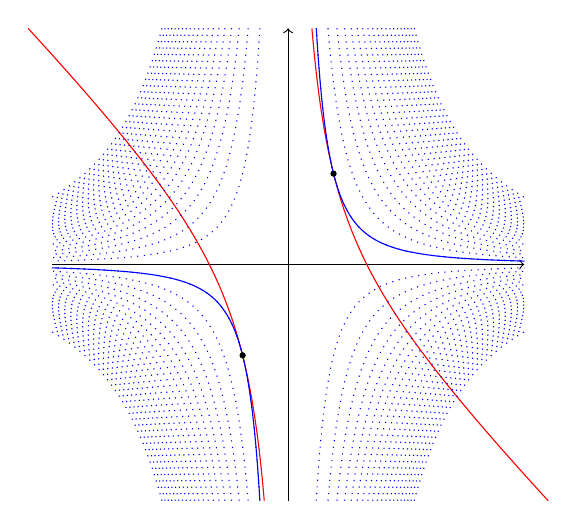
\begin{tikzpicture}
   \draw[->] (-3,0) -- (3,0);
   \draw[->] (0,-3) -- (0,3);
   \draw[red,domain=-3:3,samples=200,smooth,variable=\y]
    plot({(-\y+sqrt(\y*\y+4))/2},{\y});
   \draw[red,domain=-3:3,samples=200,smooth,variable=\y]
    plot({(-\y-sqrt(\y*\y+4))/2},{\y});
   \foreach \i in {1,...,20} {
    \def\c{0.3849*\i}
    \def\a{sqrt(\c/3)}
    \draw[dotted,blue,domain={\a}:3,samples=200,smooth,variable=\x]
     plot({\x},{\c/(\x*\x)});
    \draw[dotted,blue,domain={\a}:3,samples=200,smooth,variable=\x]
     plot({-\x},{\c/(\x*\x)});
    \draw[dotted,blue,domain={\a}:3,samples=200,smooth,variable=\x]
     plot({\x},{-\c/(\x*\x)});
    \draw[dotted,blue,domain={\a}:3,samples=200,smooth,variable=\x]
     plot({-\x},{-\c/(\x*\x)});
   }
   \def\c{0.3849}
   \def\a{sqrt(\c/3)}
   \draw[blue,domain={\a}:3,samples=200,smooth,variable=\x]
    plot({\x},{\c/(\x*\x)});
   \draw[blue,domain={\a}:3,samples=200,smooth,variable=\x]
    plot({-\x},{-\c/(\x*\x)});
   \fill ( 0.577, 1.154) circle(0.04);
   \fill (-0.577,-1.154) circle(0.04);
  \end{tikzpicture}
 \end{center}
\end{solution}

\begin{exercise}
 Locate the critical points of $f(x,y)=x^2+y^2$ subject to the
 condition $3x^2+4xy+6y^2=140$.
\end{exercise}
\begin{solution}
 We need to find the unconstrained critical points of the function
 \[ L(\lm,x,y) = x^2+y^2 - \lm(3x^2+4xy+6y^2-140). \]
 These are the points where the following equations hold:
 \begin{align*}
  L_\lm(\lm,x,y) &= 3x^2+4xy+6y^2-140 = 0 \tag{A} \\
  L_x(\lm,x,y)   &= 2x - (6x + 4y)\lm = 0 \tag{B} \\
  L_y(\lm,x,y)   &= 2y - (4x + 12y)\lm = 0. \tag{C}
 \end{align*}
 The best way to start solving these is to eliminate $\lm$ from~(B)
 and~(C).  We multiply~(B) by $4x+12y$ and~(C) by $6x+4y$ and
 then subtract.  The terms involving $\lm$ cancel out and we are left
 with $2x(4x+12y)-2y(6x+4y)=0$.  We can expand this out to get
 $8x^2+12xy-8y^2=0$, and then factorise to get $4(2x-y)(x+2y)=0$.
 This means that either $y=2x$ or $x=-2y$.  
 \begin{itemize}
  \item[(1)] Consider the case where $y=2x$.  Equation~(A) becomes
   $3x^2+4x(2x)+6(2x)^2=140$, which gives $35x^2=140$, so $x=\pm 2$.
   As $y=2x$ we see that this gives critical points (for the
   constrained problem) at $(2,4)$ and $(-2,-4)$.  At these points we
   have $f(x,y)=x^2+y^2=20$.
  \item[(2)] Now consider the other case where $x=-2y$.  Equation~(A)
   becomes $3(-2y)^2+4(-2y)y+6y^2=140$, which gives $10y^2=140$, so
   $y=\pm\sqrt{14}$.  As $x=-2y$ we see that this gives critical
   points (for the constrained problem) at $(-2\sqrt{14},\sqrt{14})$
   and $(2\sqrt{14},-\sqrt{14})$.  At these points we have
   $f(x,y)=x^2+y^2=70$.
 \end{itemize}

 For an alternative approach, we can rearrange equation~(B) to get 
 $(2-6\lm)x=4y\lm$ and so $x/y=2\lm/(1-3\lm)$.  Similarly, we can
 rearrange~(C) to get $(2-12\lm)y=4x\lm$ so $x/y=(1-6\lm)/(2\lm)$.
 Comparing these expressions gives $2\lm/(1-3\lm)=(1-6\lm)/(2\lm)$, or 
 $4\lm^2=(1-3\lm)(1-6\lm)=1-9\lm+18\lm^2$, or $14\lm^2-9\lm+1=0$.
 Using the quadratic formula we obtain $\lm=(9\pm\sqrt{25})/28$, so
 $\lm=1/2$ or $\lm=1/7$.  If $\lm=1/2$ then the equation
 $x/y=2\lm/(1-3\lm)$ gives $x=-2y$, and the rest of the calculation is
 as in case~(2) above.  If $\lm=1/7$ then the equation
 $x/y=2\lm/(1-3\lm)$ gives $y=2x$, and the rest of the calculation is
 as in case~(1) above.  

 These equations can be visualised as shown below.  The constraint
 curve (where $3x^2+4xy+6y^2=140$) is shown in red, and the contours
 of $f$ are shown in blue.  Most of them are dotted, but the contours
 where $f(x,y)=20$ and $f(x,y)=70$ are shown as solid curves.  These
 are the contours that touch the constraint curve at the critical
 points. 
 \begin{center}
  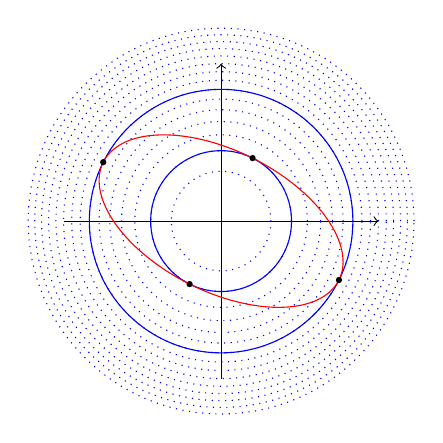
\begin{tikzpicture}[scale=0.2]
   \draw[->] (-10,0) -- (10,0);
   \draw[->] (0,-10) -- (0,10);
   \foreach \i in {1,...,15} {
    \def\r{sqrt(10*\i)}
    \draw[dotted,blue] (0,0) circle(\r);
   }
   \draw[blue] (0,0) circle({sqrt(20)});
   \draw[blue] (0,0) circle({sqrt(70)});
   \draw[red,domain=0:360,samples=200,smooth,variable=\t]
     plot({6.831*cos(\t)+3.651*sin(\t)},{-5.477*sin(\t)});
   \fill (-7.483, 3.741) circle(0.2);
   \fill ( 7.483,-3.741) circle(0.2);
   \fill ( 2, 4) circle(0.2);
   \fill (-2,-4) circle(0.2);
  \end{tikzpicture}
 \end{center}
\end{solution}

\begin{exercise}
 A triangle in the $xy$-plane has vertices at $(0,0)$, $(x,0)$ and
 $(x,y)$, with $x,y\geq 0$.  The point $(x,y)$ lies on the circle of
 radius $1$ with centre at $(1,0)$. Use the method of Lagrange
 multipliers to show that the maximum possible area for the triangle
 is $3\sqrt{3}/8$.
\end{exercise}
\begin{solution}
 The geometry is as follows:
 \begin{center}
  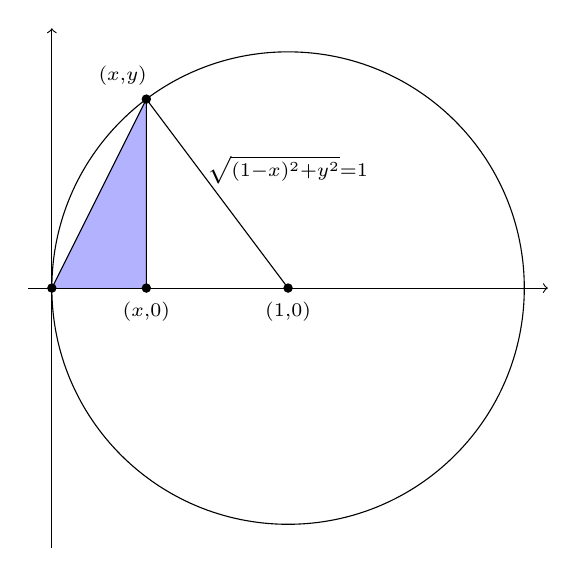
\begin{tikzpicture}[scale=3]
   \fill[blue!30] (0,0) -- (0.4,0) -- (0.4,0.8) -- (0,0);
   \draw[->] (-0.1,0) -- (2.1,0);
   \draw[->] (0,-1.1) -- (0,1.1);
   \fill (0.0,0.0) circle(0.02);
   \fill (0.4,0.0) circle(0.02);
   \fill (1.0,0.0) circle(0.02);
   \fill (0.4,0.8) circle(0.02);
   \draw (1,0) circle(1);
   \draw (0,0) -- (0.4,0.8) -- (0.4,0);
   \draw (0.40, 0.80) -- (1,0);
   \draw (0.40,-0.10) node{$\ss(x,0)$};
   \draw (1.00,-0.10) node{$\ss(1,0)$};
   \draw (0.30, 0.90) node{$\ss(x,y)$};
   \draw (1.00, 0.50) node{$\ss\sqrt{(1-x)^2+y^2}=1$};
  \end{tikzpicture}
 \end{center}
 The area of the triangle is $S=xy/2$.  Pythagoras's theorem tells us
 that the distance from $(x,y)$ to $(1,0)$ is $\sqrt{(1-x)^2+y^2}$.
 As the point is supposed to lie on the circle of radius $1$ centred
 at $(1,0)$, we must have $(1-x)^2+y^2=1$.  Our problem is thus to
 maximise $xy/2$ subject to $(1-x)^2+y^2-1=0$, so we put 
 \[ L = xy/2 - \lambda ((1-x)^2+y^2-1) = xy/2-\lm(x^2+y^2-2x). \]
 The equations for a critical point are
 \begin{align*}
  L_\lm &= 2x-x^2-y^2 = 0 \tag{A} \\
  L_x &= y/2-2\lm x+2\lm = 0 \tag{B} \\
  L_y &= x/2-2\lm y = 0. \tag{C}
 \end{align*}
 Equation~(C) gives $\lm=x/(4y)$.  (To get this we had to divide by
 $y$.  That is acceptable because it is clear that the maximum area
 does not occur when $y=0$.)  We can substitute this in~(B) we
 get $y/2-x^2/(2y)+x/(2y)=0$.  After multiplying by $2y$ this becomes
 \[ y^2-x^2+x=0. \tag{D} \]
 We now add~(A) and~(D) to get $3x-2x^2=0$.  Again, it is clear that
 $x$ is not zero when we have maximum area, so it is acceptable to
 divide this by $2x$ to get $x=3/2$.  Equation~(A) then becomes
 $y^2=3/4$, and $y\geq 0$ so $y=\sqrt{3}/2$.  Thus, the maximum area
 is $xy/2=3\sqrt{3}/8$ and occurs for $(x,y)=(3/2,\sqrt{3}/2)$.
 There are further critical points at $(0,0)$ and $(3/2,-\sqrt{3}/2)$
 but these are not relevant for the original problem.  

 The equations can be visualised as shown below.  The constraint curve
 (where $(1-x)^2+y^2=1$) is the red circle, and the contours of $xy/2$
 are shown in blue.  Most of them are dotted, but the contours where
 $xy/2=3\sqrt{3}/8$ or $xy/2=-2\sqrt{3}/8$ are shown as solid curves.
 These are the contours that touch the constraint curve at the
 critical points. 
 \begin{center}
  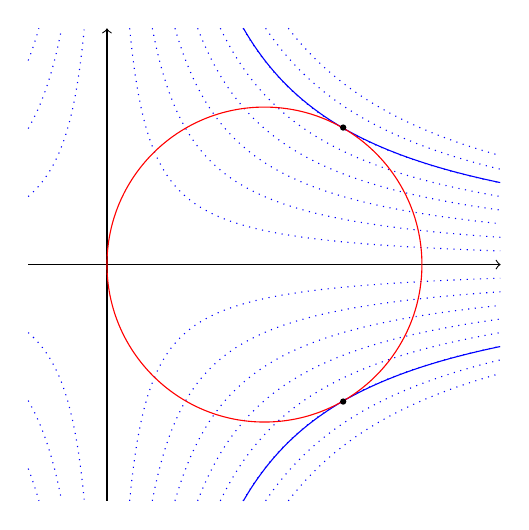
\begin{tikzpicture}[scale=2]
   \draw[->] (-0.5,0) -- (2.5,0);
   \draw[->] (0,-1.5) -- (0,1.5);
   \foreach \i in {1,...,3} {
    \def\c{0.108*\i}
    \def\a{1.333*\c}
    \draw[dotted,blue,domain={-0.5}:{-\a},samples=200,smooth,variable=\x]
     plot({\x},{2*\c/\x});
    \draw[dotted,blue,domain={-0.5}:{-\a},samples=200,smooth,variable=\x]
     plot({\x},{-2*\c/\x});
   }
   \foreach \i in {1,...,8} {
    \def\c{0.108*\i}
    \def\a{1.333*\c}
    \draw[dotted,blue,domain={\a}:2.5,samples=200,smooth,variable=\x]
     plot({\x},{2*\c/\x});
    \draw[dotted,blue,domain={\a}:2.5,samples=200,smooth,variable=\x]
     plot({\x},{-2*\c/\x});
   }
   \def\c{0.65}
   \def\a{1.333*\c}
   \draw[blue,domain={\a}:2.5,samples=200,smooth,variable=\x]
    plot({\x},{2*\c/\x});
   \draw[blue,domain={\a}:2.5,samples=200,smooth,variable=\x]
    plot({\x},{-2*\c/\x});
   \draw[red] (1,0) circle(1); 
   \fill (1.5, 0.87) circle(0.02);
   \fill (1.5,-0.87) circle(0.02);
  \end{tikzpicture}
 \end{center} 
\end{solution}

\begin{exercise}
 A solid body of volume $V$ and surface $S$ is formed by joining together
 two cubes of different sizes so that every point of a face of the smaller
 cube is in contact with the larger cube. If $S=7m^2$, use the method of
 Lagrange multipliers to find the critical value of $V$ for which both
 cubes have non-zero volumes.
\end{exercise}
\begin{solution}
 The solid body looks like this:
 \begin{center}
  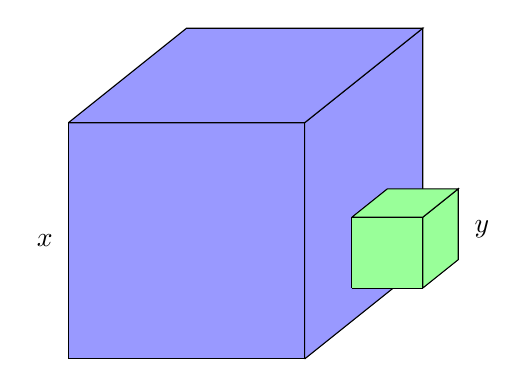
\begin{tikzpicture}[scale=3]
   \def\a{0.5}
   \def\b{0.4}
   \begin{scope}[fill=blue!40,draw=black]
    \filldraw (0,0) -- (1,0) -- (1,1) -- (0,1) -- (0,0);
    \filldraw (1,0) -- ({1+\a},\b) -- ({1+\a},{1+\b}) -- (1,1) -- (1,0);
    \filldraw (0,1) -- (1,1) -- ({1+\a},{1+\b}) -- (\a,{1+\b}) -- (0,1);
   \end{scope}
   \begin{scope}[fill=green!40,draw=black,xshift=1.2cm,yshift=0.3cm,scale=0.3]
    \filldraw (0,0) -- (1,0) -- (1,1) -- (0,1) -- (0,0);
    \filldraw (1,0) -- ({1+\a},\b) -- ({1+\a},{1+\b}) -- (1,1) -- (1,0);
    \filldraw (0,1) -- (1,1) -- ({1+\a},{1+\b}) -- (\a,{1+\b}) -- (0,1);
   \end{scope}
   \draw (-0.1,0.5) node{$x$};
   \draw (1.75,0.55) node{$y$};
  \end{tikzpicture}
 \end{center}
 We let $x$ be the length of the sides of the larger cube, and $y$ the
 length of the sides of the smaller cube, so $0<y<x$.  The surface
 consists of $5$ green faces of area $y^2$, plus five ordinary blue
 faces of order $x^2$, plus the face along which the two cubes are
 joined.  This face originally had area $x^2$ but a square of area
 $y^2$ was removed when the cubes were joined, leaving an area of
 $x^2-y^2$.  Thus, the total area is
 \[ S = 5y^2 + 5x^2 + (x^2-y^2) = 6x^2+4y^2. \]
 On the other hand, we have $V=x^3+y^3$.  Thus, we are trying to
 optimise $x^3+y^3$ subject to $6x^2+4y^2-7=0$, so we need to take
 \[ L = x^3+y^3 - \lm(6x^2+4y^2-7) = 0. \]
 The equations for a critical point are
 \begin{align*}
  L_\lm &= 7-6x^2-4y^2 = 0 \tag{A} \\
  L_x &= 3x^2-12\lm x = 3x(x-4\lm) = 0 \tag{B} \\
  L_y &= 3y^2-8\lm y = 3y(y-8\lm/3) = 0. \tag{C}
 \end{align*}
 We are asked to find a critical point where both cubes have nonzero
 size, so $x,y>0$.  It is therefore legitimate to divide~(B) and~(C)
 by $3x$ and $3y$, giving $x=4\lm$ and $y=8\lm/3$ (and so $\lm>0$).
 Substituting these into~(A) gives $96\lm^2+256\lm^2/9=7$, so
 $1120\lm^2=63$, so 
 \[ \lm=\sqrt{63/1120}=\frac{3}{4\sqrt{10}}\simeq 0.237. \]
 From this we get $x=4\lm\simeq 0.949$ and $y=8\lm/3\simeq 0.632$ and
 $V=x^3+y^3\simeq 1.107$.

 \begin{center}
  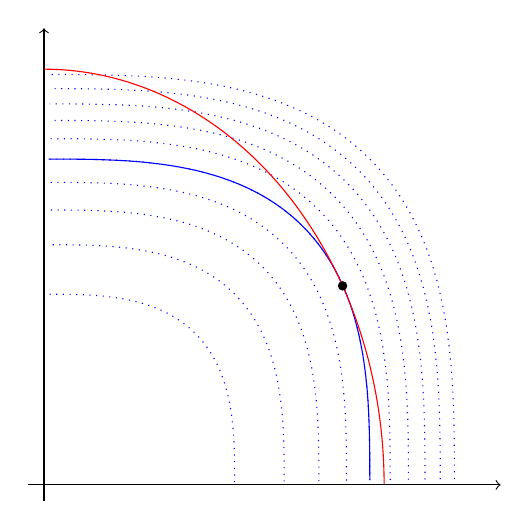
\begin{tikzpicture}[scale=4]
   \draw[->] (-0.05,0) -- (1.45,0);
   \draw[->] (0,-0.05) -- (0,1.45);
   \foreach \i in {1,...,10} {
    \def\r{exp(0.333*ln(0.2214*\i))}
    \draw[dotted,blue,domain=0.1:89.9,samples=200,smooth,variable=\t]
     plot({\r*exp(0.666*ln(cos(\t)))},{\r*exp(0.666*ln(sin(\t)))});  
   }
   \def\r{exp(0.333*ln(1.107))}
   \draw[blue,domain=0.1:89.9,samples=200,smooth,variable=\t]
    plot({\r*exp(0.666*ln(cos(\t)))},{\r*exp(0.666*ln(sin(\t)))});  
   \draw[red,domain=0.1:89.9,samples=200,smooth,variable=\t]
    plot({1.08*cos(\t)},{1.32*sin(\t)});
   \fill (0.948,0.632) circle(0.015);
  \end{tikzpicture}
 \end{center} 
\end{solution}

\section*{Week 3 --- Integrals over plane regions}

\begin{exercise}
 Evaluate the following integrals, and sketch the corresponding
 regions in the $(x,y)$-plane. 
 \begin{itemize}
  \item[(a)] $\int_{x=-1}^1\int_{y=-2}^2(2x^2+y^2)\,dy\,dx$
  \item[(b)] $\int_{x=1}^2\int_{y=0}^1x\,e^y\,dy\,dx$
  \item[(c)] $\int_{x=2/a}^{4/a}\int_{y=1/x}^a y^2\,dy\,dx$
  \item[(d)] $\int_{y=0}^\pi\int_{x=0}^{\sin(y)} 1\,dx\,dy$.
 \end{itemize}
\end{exercise}
\begin{solution}
 \begin{itemize}
  \item[(a)]
   \begin{minipage}[t]{11cm}
     \begin{align*}
       & \int_{x=-1}^1\int_{y=-2}^2(2x^2+y^2)\,dy\,dx \\
       =&\int_{x=-1}^1\CH{2x^2y+y^3/3}_{y=-2}^2\,dx \\
       =&\int_{x=-1}^1(8x^2+16/3)dx \\
       =&\CH{8x^3/3+16x/3}_{x=-1}^1=24/3-(-24/3)=16.
     \end{align*}\hfill
   \end{minipage} \hfill \parbox[t]{5cm}{
     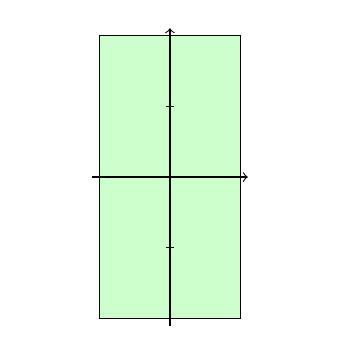
\begin{tikzpicture}[scale=0.9,baseline=(current bounding box.north)]
      \draw[white] (-2,0) -- (2,0);
      \filldraw[fill=green!20,draw=black] (-1,-2) rectangle(1,2);
      \draw[->] (-1.1,0) -- (1.1,0);
      \draw[->] (0,-2.1) -- (0,2.1);
      \draw (-0.05,-1) -- (0.05,-1);
      \draw (-0.05,+1) -- (0.05,+1);
     \end{tikzpicture}
   }\\[2ex]
  \item[(b)]
   \begin{minipage}[t]{11cm}
     \begin{align*}
      & \int_{x=1}^2\int_{y=0}^1x\,e^y\,dy\,dx \\
     =& \int_{x=1}^2\CH{x\,e^y}_{y=0}^1\,dx \\
     =& \int_{x=1}^2(e-1)x\,dx=\CH{(e-1)x^2/2}_{x=1}^2 \\ 
     =& (e-1)(4/2-1/2)=3(e-1)/2.
     \end{align*}\hfill
   \end{minipage} \hfill \parbox[t]{5cm}{
     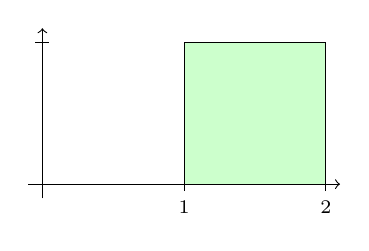
\begin{tikzpicture}[scale=1.8,baseline=(current bounding box.north)]
      \filldraw[fill=green!20,draw=black] (1,0) rectangle(2,1);
      \draw[->] (-0.1,0) -- (2.1,0);
      \draw[->] (0,-0.1) -- (0,1.1);
      \draw (1,-0.05) -- (1,0.05);
      \draw (2,-0.05) -- (2,0.05);
      \draw (-0.05,+1) -- (0.05,+1);
      \draw (1,-0.05) node[anchor=north]{$\ss 1$};
      \draw (2,-0.05) node[anchor=north]{$\ss 2$};
     \end{tikzpicture}
   }\\[2ex]
  \item[(c)]
   \begin{minipage}[t]{11cm}
     \begin{align*}
       & \int_{x=2/a}^{4/a}\int_{y=1/x}^a y^2\,dy\,dx \\
      =& \int_{x=2/a}^{4/a}\CH{\frac{y^3}{3}}_{y=1/x}^a\,dx \\
      =& \frac{1}{3}\int_{x=2/a}^{4/a}a^3-x^{-3}\,dx \\
      =& \frac{1}{3}\CH{a^3x+\frac{1}{2}x^{-2}}_{x=2/a}^{4/a} \\
      =& \frac{1}{3}((4a^2+a^2/32)-(2a^2+a^2/8))=61a^2/96
     \end{align*}\hfill
   \end{minipage} \hfill \parbox[t]{5cm}{
     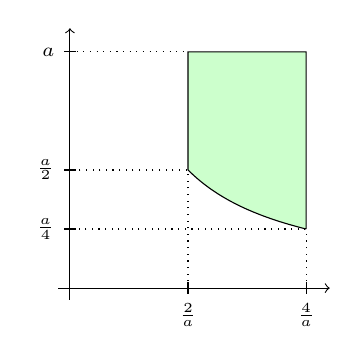
\begin{tikzpicture}[scale=1.5,baseline=(current bounding box.north)]
      \def\a{2}
      \draw[dotted] ({4/\a},0) -- ({4/\a},{\a/4}) -- (0,{\a/4});
      \draw[dotted] ({2/\a},0) -- ({2/\a},{\a/2}) -- (0,{\a/2});
      \draw[dotted] (0,{\a}) -- ({2/\a},\a);
      \filldraw[fill=green!20,draw=black,domain={2/\a}:{4/\a},samples=200,smooth,variable=\x]
       ({4/\a},{\a/4}) -- ({4/\a},\a) -- ({2/\a},\a) --
        plot(\x,{1/\x}); 
      \draw[->] (-0.1,0) -- ({4.4/\a},0);
      \draw[->] (0,-0.1) -- (0,1.1*\a);
      \draw ({2/\a},-0.05) -- ({2/\a},0.05);
      \draw ({4/\a},-0.05) -- ({4/\a},0.05);
      \draw (-0.05,{\a/4}) -- (0.05,{\a/4});
      \draw (-0.05,{\a/2}) -- (0.05,{\a/2});
      \draw (-0.05,{\a}  ) -- (0.05,{\a}  );
      \draw ({2/\a},-0.05) node[anchor=north]{$\ss\frac{2}{a}$};
      \draw ({4/\a},-0.05) node[anchor=north]{$\ss\frac{4}{a}$};
      \draw (-0.05,{\a  }) node[anchor=east]{$\ss a$};
      \draw (-0.05,{\a/2}) node[anchor=east]{$\ss\frac{a}{2}$};
      \draw (-0.05,{\a/4}) node[anchor=east]{$\ss\frac{a}{4}$};
     \end{tikzpicture}
   }\\[2ex]
  \item[(d)]
   \begin{minipage}[t]{11cm}
     \begin{align*}
       & \int_{y=0}^\pi\int_{x=0}^{\sin(y)} 1\,dx\,dy \\
      =& \int_{y=0}^\pi\sin(y) \,dx\,dy \\
      =& \CH{-\cos(y)}_{y=0}^{\pi} \\
      =& 1 - (-1) = 2.
     \end{align*}\hfill
   \end{minipage} \hfill \parbox[t]{5cm}{
     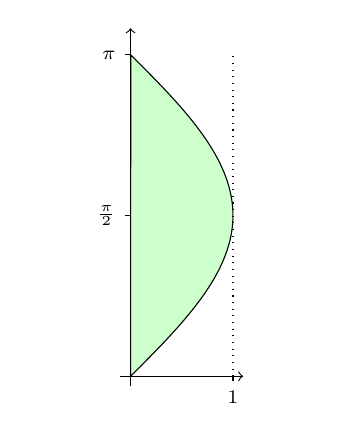
\begin{tikzpicture}[scale=1.3,baseline=(current bounding box.north)]
      \draw[white] (-1,0) -- (2,0);
      \draw[->] (-0.1,0) -- (1.1,0);
      \draw[->] (0,-0.1) -- (0,3.4);
      \filldraw[fill=green!20,draw=black,domain=0:3.14,samples=200,smooth,variable=\y]
        plot({sin(57.3*\y)},{\y}) -- (0,0);
      \draw[dotted] (1,0) -- (1,3.14);
      \draw (1,0) -- (1,-0.05);
      \draw (-0.05,1.57) -- (0,1.57);
      \draw (-0.05,3.14) -- (0,3.14);
      \draw (1,-0.05) node[anchor=north] {$\ss 1$}; 
      \draw (-0.05,3.14) node[anchor=east] {$\ss \pi$}; 
      \draw (-0.05,1.57) node[anchor=east] {$\ss\frac{\pi}{2}$}; 
     \end{tikzpicture}
   }
 \end{itemize}
\end{solution}

\begin{exercise}
 Express the following double integrals as repeated integrals and
 evaluate them: 
 \begin{itemize}
  \item[(a)] $\iint_D xy\,dA$, where $D$ is the rectangle bounded by
   the lines $x=0$, $x=a$, $y=0$ and $y=b$.
  \item[(b)] $\iint_D e^{x+y}\,dA$, where $D$ is the region bounded by
   the lines $x=0$, $y=0$ and $x+y=1$.
  \item[(c)] $\iint_D e^{y^2}\,dA$, where $D$ is the triangle with
   vertices $(0,0)$, $(-1,1)$ and $(1,1)$.
  \item[(d)] $\iint_D x^2\,dA$, where $D$ is the trapezium with
   vertices $(-1,0)$, $(1,0)$, $(0,1)$ and $(1,1)$.
 \end{itemize}
\end{exercise}
\begin{solution}
 \begin{itemize}
  \item[(a)]
   \begin{minipage}[t]{11cm}
     \begin{align*}
      \iint_D xy\,dA &= 
       \int_{x=0}^a \int_{y=0}^b xy\,dy\,dx \\
      &= \int_{x=0}^a\CH{\half xy^2}_{y=0}^b\,dx 
       = \int_{x=0}^a \half xb^2 \,dx \\
      &= \CH{\tfrac{1}{4}x^2b^2}_{x=0}^a = \frac{a^2b^2}{4}.
     \end{align*}
   \end{minipage} \hfill \parbox[t]{5cm}{
     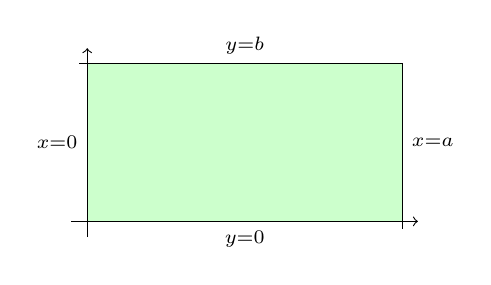
\begin{tikzpicture}[scale=2,baseline=(current bounding box.north)]
      \def\a{2} \def\b{1}
      \fill[green!20] (0,0) rectangle (\a,\b);
      \draw[->] (-0.1,0) -- ({\a+0.1},0);
      \draw[->] (0,-0.1) -- (0,{\b+0.1});
      \draw (-0.05,\b) -- (\a,\b) -- (\a,-0.05);
      \draw ({\a/2},0)  node[anchor=north] {$\ss y=0$};
      \draw ({\a/2},\b) node[anchor=south] {$\ss y=b$};
      \draw (0,{\b/2})  node[anchor=east]  {$\ss x=0$};
      \draw (\a,{\b/2}) node[anchor=west]  {$\ss x=a$};
     \end{tikzpicture}
   }\\[2ex]
  \item[(b)] 
   \begin{minipage}[t]{11cm}
     \begin{align*}
      \iint_D e^{x+y}\,dA
       &= \int_{x=0}^1\int_{y=0}^{1-x} e^{x+y}dy\,dx \\
       &= \int_{x=0}^1\CH{e^{x+y}}_{y=0}^{1-x}\,dx 
        = \int_{x=0}^1 e-e^x \,dx \\
       &= \CH{ex-e^x}_{x=0}^1 = (e-e)-(0-1) = 1.
     \end{align*}
   \end{minipage} \hfill \parbox[t]{5cm}{
     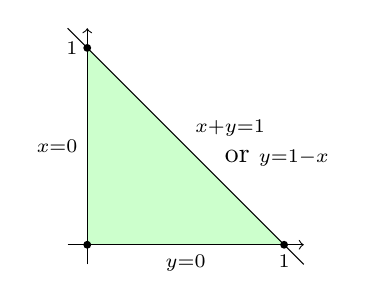
\begin{tikzpicture}[scale=2.5,baseline=(current bounding box.north)]
      \fill[green!20] (0,0) -- (1,0) -- (0,1) -- (0,0);
      \draw[->] (-0.1,0) -- (1.1,0);
      \draw[->] (0,-0.1) -- (0,1.1);
      \draw (-0.1,1.1) -- (1.1,-0.1);
      \fill (0,0) circle(0.02);
      \fill (1,0) circle(0.02);
      \fill (0,1) circle(0.02);
      \draw (0.5,0) node[anchor=north] {$\ss y=0$};
      \draw (0,0.5) node[anchor=east]  {$\ss x=0$};
      \draw (1,0) node[anchor=north]  {$\ss 1$};
      \draw (0,1) node[anchor=east]   {$\ss 1$};
      \draw (0.50,0.50) node[anchor=south west] {$\ss x+y=1$};
      \draw (0.65,0.35) node[anchor=south west] {or $\ss y=1-x$};
     \end{tikzpicture}
   }\\[2ex]
  \item[(c)] 
   \begin{minipage}[t]{11cm}
     \begin{align*}
      \iint_D e^{y^2}\,dA
       &= \int_{y=0}^1\int_{x=-y}^y e^{y^2}\,dx\,dy 
        = \int_{y=0}^1 e^{y^2}.2y\,dy \\
       &= \int_{u=0}^1 e^u \,du
          \hspace{5em} (u=y^2,\;du=2y\,dy) \\
       &= \CH{e^u}_{u=0}^1 = e-1.
     \end{align*}
   \end{minipage} \hfill \parbox[t]{5cm}{
     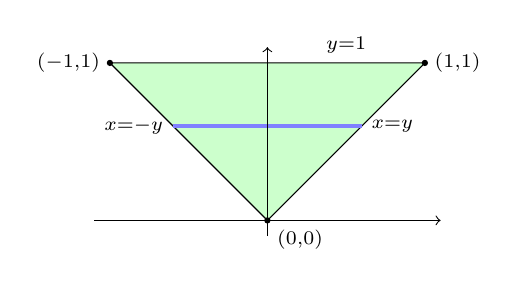
\begin{tikzpicture}[scale=2,baseline=(current bounding box.north)]
      \filldraw[fill=green!20,draw=black] (0,0) -- (-1,1) -- (1,1) -- (0,0);
      \draw[ultra thick,blue!50] (-0.6,0.6) -- (0.6,0.6);
      \draw[->] (-1.1,0) -- (1.1,0);
      \draw[->] (0,-0.1) -- (0,1.1);
      \fill ( 0,0) circle(0.02);
      \fill (-1,1) circle(0.02);
      \fill ( 1,1) circle(0.02);
      \draw (-1,1) node[anchor=east] {$\ss (-1,1)$};
      \draw ( 1,1) node[anchor=west] {$\ss (1,1)$};
      \draw ( 0,0) node[anchor=north west] {$\ss (0,0)$};
      \draw (-0.6,0.6) node[anchor=east] {$\ss x=-y$};
      \draw ( 0.6,0.6) node[anchor=west] {$\ss x=y$};
      \draw ( 0.5,1.0) node[anchor=south] {$\ss y=1$};
     \end{tikzpicture}
   }\\[2ex]
   We could alternatively try to do this using vertical strips, but
   then we would need to do the left half and the right half
   separately and add them together.  The left half would be
   $\int_{x=-1}^0\int_{y=-x}^1e^{y^2}\,dy\,dx$, and the right half
   would be $\int_{x=0}^1\int_{y=x}^1e^{y^2}\,dy\,dx$.  The inner
   integral $\int e^{y^2}\,dy$ cannot be expressed in terms of
   familiar functions, so this is not a useful approach.
  \item[(d)] 
   \begin{minipage}[t]{11cm}
     First, we have
     \[ \iint_D x^2\,dA = \int_{y=0}^1\int_{x=y-1}^1 x^2\,dx\,dy. \]
     The inner integral is
     \begin{align*}
      \int_{x=y-1}^1 x^2\,dx 
       &= \CH{\frac{x^3}{3}}_{x=y-1}^1 
        = \tfrac{1}{3}(1 - (y-1)^3) \\
       &= \tfrac{1}{3}(1 - y^3 + 3y^2 - 3y + 1) \\
       &= \tfrac{2}{3} - \tfrac{1}{3} y^3 + y^2 - y.  
     \end{align*}
     Putting this into the outer integral gives
     \begin{align*}
      \iint_D x^2\,dA 
      &= \int_{y=0}^1(\tfrac{2}{3} - \tfrac{1}{3} y^3 + y^2 - y)\,dy \\
      &= \CH{\tfrac{2}{3}y - \tfrac{1}{12} y^4 +
             \tfrac{1}{3}y^3 - \tfrac{1}{2}y^2}_0^1 
       = \tfrac{2}{3} - \tfrac{1}{12} + \tfrac{1}{3} - \tfrac{1}{2} \\
      &= 5/12.
     \end{align*}
   \end{minipage} \hfill \parbox[t]{5cm}{
     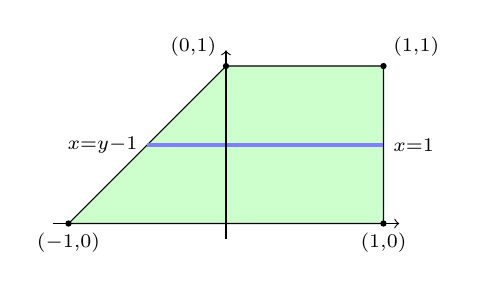
\begin{tikzpicture}[scale=2,baseline=(current bounding box.north)]
      \filldraw[fill=green!20,draw=black] 
       (-1,0) -- (1,0) -- (1,1) -- (0,1) -- (-1,0);
      \draw[ultra thick,blue!50] (-0.5,0.5) -- (1,0.5);
      \draw[->] (-1.1,0) -- (1.1,0);
      \draw[->] (0,-0.1) -- (0,1.1);
      \fill (-1,0) circle(0.02);
      \fill ( 1,0) circle(0.02);
      \fill ( 1,1) circle(0.02);
      \fill ( 0,1) circle(0.02);
      \draw (-1,0) node[anchor=north] {$\ss (-1,0)$};
      \draw ( 1,0) node[anchor=north] {$\ss ( 1,0)$};
      \draw ( 1,1) node[anchor=south west] {$\ss ( 1,1)$};
      \draw ( 0,1) node[anchor=south east] {$\ss ( 0,1)$};
      \draw (-0.5,0.5) node[anchor=east] {$\ss x=y-1$};
      \draw ( 1.0,0.5) node[anchor=west] {$\ss x=1$};
     \end{tikzpicture}
   }\\[2ex]
   We could alternatively do this using vertical strips, but
   then we would need to do the left half and the right half
   separately and add them together.  The left half would be
   $\int_{x=-1}^0\int_{y=0}^{1+x}x^2\,dy\,dx=\int_{x=-1}^0(x^2+x^3)\,dx=\frac{1}{12}$,
   and the right half would be
   $\int_{x=0}^1\int_{y=0}^1x^2\,dy\,dx=\frac{1}{3}$ giving
   $\frac{1}{12}+\frac{1}{3}=\frac{5}{12}$ overall as before.
 \end{itemize}
\end{solution}

\begin{exercise}
 By sketching the region of integration, show that 
 \[ \int_{y=0}^1\int_{x=\sqrt{y}}^1 1\,dx\,dy = 
     \int_{x=0}^1\int_{y=0}^{x^2}1\,dy\,dx.
 \]
 Evaluate both integrals and check that they are the same.
\end{exercise}
\begin{solution}
 The region is as follows:
 \begin{center}
  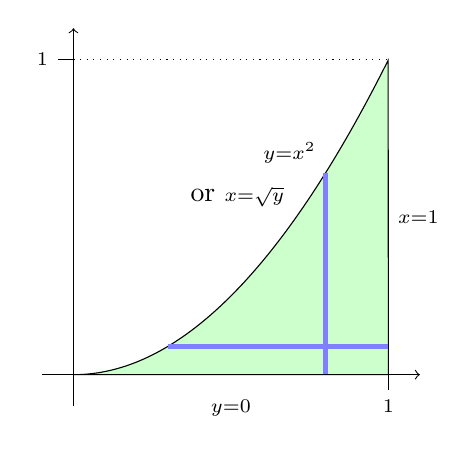
\begin{tikzpicture}[scale=4,baseline=(current bounding box.north)]
   \filldraw[fill=green!20,draw=black,domain=0:1,samples=200,smooth,variable=\x]
    plot(\x,{\x*\x}) -- (1,0) -- (0,0);
   \draw[ultra thick,blue!50] (0.8,0) -- (0.8,0.64);
   \draw[ultra thick,blue!50] (0.3,0.09) -- (1,0.09);
   \draw[->] (-0.1,0) -- (1.1,0);
   \draw[->] (0,-0.1) -- (0,1.1); 
   \draw (1,0) -- (1,-0.05);
   \draw (0,1) -- (-0.05,1);
   \draw[dotted] (0,1) -- (1,1);
   \draw (1,-0.05) node[anchor=north] {$\ss 1$};
   \draw (-0.05,1) node[anchor=east]  {$\ss 1$};
   \draw (0.5,-0.05) node[anchor=north]  {$\ss y=0$};
   \draw (1,0.5) node[anchor=west]  {$\ss x=1$};
   \draw (0.8,0.64) node[anchor=south east] {$\ss y=x^2$};
   \draw (0.7,0.50) node[anchor=south east] {or $\ss x=\sqrt{y}$};
  \end{tikzpicture}
 \end{center}
 The horizontal slice at height $y$ runs from $x=\sqrt{y}$ to $x=1$,
 in accordance with the limits in the left hand integral.  The
 vertical slice at position $x$ runs from $y=0$ to $y=x^2$, in
 accordance with the limits in the right hand integral.  Thus, the two
 integrals should be the same.  We can evaluate them as follows:
 \begin{align*}
  \int_{y=0}^1\int_{x=\sqrt{y}}^1 1\,dx\,dy
   &= \int_{y=0}^1 1-\sqrt{y} \,dy = \int_{y=0}^1 1-y^{\frac{1}{2}} \,dy\\ 
   &= \CH{y-\tfrac{2}{3}y^{\tfrac{3}{2}}}_{y=0}^1 = 1-\tfrac{2}{3}
    = \tfrac{1}{3} \\
  \int_{x=0}^1\int_{y=0}^{x^2}1\,dy\,dx 
   &= \int_{x=0}^1 x^2\, dx = \CH{\tfrac{1}{3}x^3}_{x=0}^1 = \tfrac{1}{3}.
 \end{align*}
\end{solution}

\begin{exercise}
 Sketch the region of the $(x,y)$-plane over which the integral 
 \[ I = \int_{x=0}^1 \int_{y=1}^{x^2+1} f(x,y)\,dy\,dx \]
 is taken.  Obtain a similar expression for $I$ by reversing the order
 of integration.
\end{exercise}
\begin{solution}\ \\
 \begin{minipage}[t]{11cm}
  The picture as shown on the right.
  The equation $y=x^2+1$ for the curved edge can be rewritten as
  $x=\sqrt{y-1}$.  Thus, we can divide the region into horizontal
  stripes running from $x=\sqrt{y-1}$ to $x=1$ for $1\leq y\leq 2$.
  This gives
  \[ I = \int_{y=1}^2 \int_{x=\sqrt{y-1}}^{1} f(x,y)\,dx\,dy. \]
 \end{minipage} \hfill \parbox[t]{5cm}{
  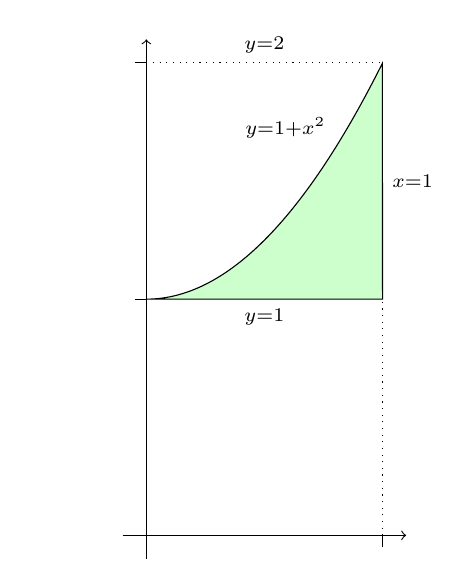
\begin{tikzpicture}[scale=3,baseline=(current bounding box.north)]
   \draw[white] (-0.5,0) -- (0,0);
   \filldraw[fill=green!20,draw=black,domain=0:1,samples=200,smooth,variable=\x]
    plot(\x,{1+\x*\x}) -- (1,1) -- (0,1);
   \draw[->] (-0.1,0) -- (1.1,0);
   \draw[->] (0,-0.1) -- (0,2.1); 
   \draw (1,-0.05) -- (1,0);
   \draw (-0.05,1) -- (0,1);
   \draw (-0.05,2) -- (0,2);
   \draw[dotted] (1,0) -- (1,1);
   \draw[dotted] (0,2) -- (1,2);
   \draw (0.5,1) node[anchor=north] {$\ss y=1$};
   \draw (0.5,2) node[anchor=south] {$\ss y=2$};
   \draw (1,1.5) node[anchor=west] {$\ss x=1$};
   \draw (0.8,1.64) node[anchor=south east]{$\ss y=1+x^2$};
  \end{tikzpicture}
 }
\end{solution}

\begin{exercise}
 Change the order of integration in the following integrals, and hence
 evaluate them:
 \begin{itemize}
  \item[(a)] $\displaystyle \int_{y=0}^\infty\int_{x=y}^\infty\frac{e^{-x}}{x}dx\,dy$
  \item[(b)] $\displaystyle \int_{x=0}^a\int_{y=x}^a\frac{y^2}{(x^2+y^2)^{1/2}}dy\,dx$
 \end{itemize}
 You may find the following integral useful:
 \[ \int \frac{1}{(x^2+y^2)^{1/2}} dx = \ln(x+\sqrt{x^2+y^2}). \]
\end{exercise}
\begin{solution}\ \\
 \begin{itemize}
  \item[(a)]  
   \begin{minipage}[t]{11cm}
    Horizontal slices run from $x=y$ to $x=\infty$.  Vertical slices
    run from $y=0$ to $y=x$.  The integral can therefore be rewritten
    as 
    \begin{align*}
     \int_{x=0}^\infty \int_{y=0}^x \frac{e^{-x}}{x}\,dy\,dx 
      &= \int_{x=0}^\infty \CH{y\frac{e^{-x}}{x}}_{y=0}^x\,dx 
       = \int_{x=0}^\infty e^{-x}\,dx \\
      &= \CH{-e^{-x}}_{x=0}^\infty = ((-0)-(-1)) = 1.
    \end{align*}
   \end{minipage} \hfill \parbox[t]{5cm}{
     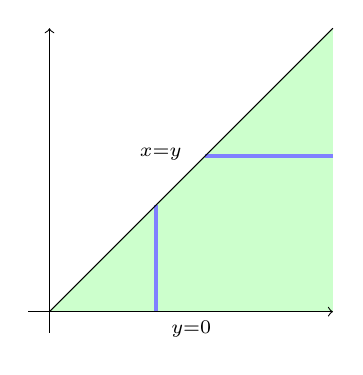
\begin{tikzpicture}[scale=0.9,baseline=(current bounding box.north)]
      \fill[green!20] (0,0) -- (4,0) -- (4,4) -- (0,0);
      \draw[blue!50,ultra thick] (1.5,0) -- (1.5,1.5);
      \draw[blue!50,ultra thick] (2.2,2.2) -- (4,2.2);
      \draw[->] (-0.3,0) -- (4,0);
      \draw[->] (0,-0.3) -- (0,4);
      \draw (0,0) -- (4,4);
      \draw (2,0) node[anchor=north] {$\ss y=0$};
      \draw (2,2) node[anchor=south east] {$\ss x=y$};
     \end{tikzpicture}
   }\\[2ex]
  \item[(b)]  
   \begin{minipage}[t]{11cm}
    Vertical slices run from $y=x$ to $y=a$.  Horizontal slices run
    from $x=0$ to $x=y$.  The integral can therefore be rewritten
    as 
    \[ I = \int_{y=0}^a \int_{x=0}^y \frac{y^2}{(x^2+y^2)^{1/2}}dx\,dy
    \]
    Using the hint, the inner integral gives
    \begin{align*}
     \int_{x=0}^y \frac{y^2}{(x^2+y^2)^{1/2}}dx
      &= \CH{y^2\ln(x+\sqrt{x^2+y^2})}_{x=0}^y \\
      &= y^2\ln(y+\sqrt{2y^2}) - y^2\ln(0+\sqrt{y^2}) \\
      &= y^2(\ln((1+\sqrt{2})y)-\ln(y)) \\
      &= y^2(\ln(1+\sqrt{2})+\ln(y)-\ln(y)) \\
      &= y^2\ln(1+\sqrt{2}).
    \end{align*}
    Note here that $\ln(1+\sqrt{2})$ is just a constant, approximately
    $0.881$.  The outer integral is now easy:
    \[ I = \int_{y=0}^a y^2\ln(1+\sqrt{2})\,dy 
        = \CH{\ln(1+\sqrt{2})y^3/3}_{y=0}^a = \frac{\ln(1+\sqrt{2})a^3}{3}.
    \]
   \end{minipage} \hfill \parbox[t]{5cm}{
    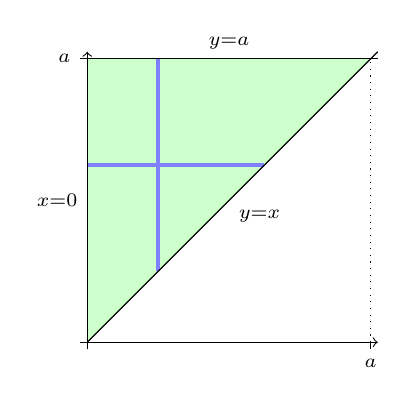
\begin{tikzpicture}[scale=0.9,baseline=(current bounding box.north)]
     \def\a{4}
     \fill[green!20] (0,0) -- (\a,\a) -- (0,\a);
     \draw[blue!50,ultra thick] (1,1) -- (1,\a);
     \draw[blue!50,ultra thick] (0,2.5) -- (2.5,2.5);
     \draw[->] (-0.1,0) -- ({0.1+\a},0);
     \draw[->] (0,-0.1) -- (0,{0.1+\a});
     \draw (0,0) -- ({0.1+\a},{0.1+\a});
     \draw (-0.1,\a) -- ({0.1+\a},\a);
     \draw[dotted] (\a,0) -- (\a,\a);
     \draw (\a,0) -- (\a,-0.1);
     \draw (\a,-0.1) node[anchor=north] {$\ss a$};
     \draw (-0.1,\a) node[anchor=east ] {$\ss a$};
     \draw ({\a/2},{\a/2}) node[anchor=north west]{$\ss y=x$};
     \draw (     0,{\a/2}) node[anchor=east]{$\ss x=0$};
     \draw ({\a/2},\a    ) node[anchor=south]{$\ss y=a$};
    \end{tikzpicture}
   }
 \end{itemize}
\end{solution}

\section*{Week 4 --- Plane polar integrals and volume integrals}

\begin{exercise}
 Consider the integral given in polar coordinates by
 $I=\int_{\tht=0}^{\pi/2}\int_{r=0}^1r^2\sin(\tht)\,dr\,d\tht$. 
 Sketch the corresponding region in the $(x,y)$-plane, and evaluate
 the integral.
\end{exercise}
\begin{solution}
  \begin{minipage}[t]{11cm}
    \begin{align*}
     I &= \int_{\tht=0}^{\pi/2}\int_{r=0}^1r^2\sin(\tht)\,dr\,d\tht \\
       &= \int_{\tht=0}^{\pi/2}\frac{1}{3}\sin(\tht)\,d\tht \\
       &= \CH{-\frac{1}{3}\cos(\tht)}_{\tht=0}^{\pi/2} \\
       &= 0 - (-\tfrac{1}{3}) = 1/3.
    \end{align*}
  \end{minipage} \hfill \parbox[t]{5cm}{
    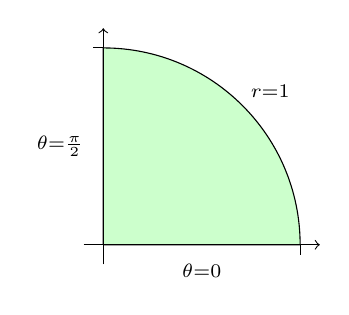
\begin{tikzpicture}[scale=2.5,baseline=(current bounding box.north)]
     \draw[->] (-0.1,0) -- (1.1,0);
     \draw[->] (0,-0.1) -- (0,1.1);
     \filldraw[fill=green!20,draw=black]
       (0,0) -- (1,0) arc(0:90:1) -- (0,0);
     \draw (1,0) -- (1,-0.05);
     \draw (0,1) -- (-0.05,1);
     \draw (0.5,-0.05) node[anchor=north] {$\ss\tht=0$}; 
     \draw (-0.05,0.5) node[anchor=east] {$\ss\tht=\frac{\pi}{2}$}; 
     \draw (0.7,0.7) node[anchor=south west] {$\ss r=1$}; 
    \end{tikzpicture}
  } 
\end{solution}

\begin{exercise}
 Evaluate $\displaystyle \iint_D xy\,dA$, where $D$ is the quadrant of
 the disk $x^2+y^2\leq a^2$ where $x\geq 0$ and $y\geq 0$.  (Hint: use
 polar coordinates.)
\end{exercise}
\begin{solution}
 The region is given in polar coordinates by the limits
 $0\leq\tht\leq\pi/2$ and $0\leq r\leq a$.  We also have
 $x=r\cos(\tht)$ and $y=r\sin(\tht)$ and $dA=r\,dr\,d\tht$ so 
 \[ xy\,dA = r^3\sin(\tht)\cos(\tht)\,dr\,d\tht =
     \half r^3\sin(2\tht) \,dr\,d\tht.
 \]
 This gives
 \begin{align*}
  \iint_D xy\,dA 
   &= \frac{1}{2}\int_{\tht=0}^{\frac{\pi}{2}}\int_{r=0}^a 
       r^3 \sin(2\tht)\,dr\,d\tht
    = \frac{a^4}{8} \int_{\tht=0}^{\frac{\pi}{2}}\sin(2\tht)\,d\tht \\
   &= \frac{a^4}{8} \CH{-\frac{\cos(2\tht)}{2}}_{\tht=0}^{\frac{\pi}{2}}
    = \frac{a^4}{16}(1-(-1)) = \frac{a^4}{8}.
 \end{align*}
\end{solution}

\begin{exercise}
 Evaluate the following integrals, where $D$ is the region given by
 $x^2+y^2\leq a^2$.
 \begin{itemize}
  \item[(a)] $\displaystyle \iint_D(x^2+y^2)^{\half}\,dA$
  \item[(b)] $\displaystyle \iint_D e^{-(x^2+y^2)}\,dA$.
 \end{itemize}
\end{exercise}
\begin{solution}
 We will use polar coordinates, so $x^2+y^2=r^2$ and
 $dA=r\,dr\,d\tht$.  The relevant limits are $0\leq r\leq a$ and
 $0\leq\tht\leq 2\pi$.  For part~(a) we have
 \[ \iint_D(x^2+y^2)^{\half}dA 
    = \int_{r=0}^a\int_{\tht=0}^{2\pi} r^2\,dr\,d\tht
    = 2\pi\int_{r=0}^ar^2\,dr = \frac{2\pi a^3}{3}
 \]
 Similarly, for part~(b) we have
 \[ \iint_D e^{-(x^2+y^2)}\,dA 
    = \int_{r=0}^a\int_{\tht=0}^{2\pi} e^{-r^2}r\,dr\,d\tht.
    = \int_{r=0}^a e^{-r^2}2\pi r\,dr\,d\tht.
 \]
 We now substitute $u=r^2$, so $du=2r\,dr$ and the limits
 $0\leq r\leq a$ become $0\leq u\leq a^2$.  The integral becomes
 \[ \int_{u=0}^{a^2} e^{-u} \pi\,du = 
     \CH{-\pi e^{-u}}_{u=0}^{a^2} = \pi(1-e^{-a^2}).
 \]
\end{solution}

\begin{exercise}
 Evaluate $\iint_D x^2\,dA$, where $D$ is the ring-shaped region
 given by $4\leq x^2+y^2\leq 9$. 
\end{exercise}
\begin{solution}
 In polar coordinates the region is described by $4\leq r^2\leq 9$ or
 equivalently $2\leq r\leq 3$, with $\tht$ running from $0$ to $2\pi$
 as usual.  We can write the integrand $x^2$ as $r^2\cos^2(\tht)$ and
 we also have $dA=r\,dr\,d\tht$.  This gives 
 \[ \iint_D x^2\,dA
    = \int_{\tht=0}^{2\pi}\int_{r=2}^3
        r^3\cos^2(\tht) \,dr\,d\tht.
 \]
 The integrand is just a function of $r$ times a function of $\tht$
 and the limits are constants so the integral breaks apart giving 
 \begin{align*}
  \iint_D x^2\,dA
   &= \left(\int_{\tht=0}^{2\pi}\cos^2(\tht)d\tht\right)
      \left(\int_{r=2}^3r^3 \,dr\right) \\
   &= \CH{\tfrac{1}{4}\cos(2\tht)+\tfrac{1}{2}\tht}_{\tht=0}^{2\pi}
      \CH{\tfrac{1}{4}r^4}_{r=2}^3 \\
   &= \pi \tm (3^4 - 2^4)/4 = 65\pi/4.
 \end{align*}
\end{solution}

\begin{exercise}
 Use polar coordinates to evaluate 
 $\displaystyle \iint_D e^{-\sqrt{x^2+y^2}}\,dA$, where $D$ is the
 region given by $x\geq 0$.
\end{exercise}
\begin{solution}
 The region is given in polar coordinates by
 $-\frac{\pi}{2}\leq\tht\leq\frac{\pi}{2}$ and $0\leq r<\infty$.  We
 therefore have 
 \[ \iint_D e^{-\sqrt{x^2+y^2}}\,dA = 
      \int_{r=0}^\infty\int_{\tht=-\frac{\pi}{2}}^{\frac{\pi}{2}}
       e^{-r}\,r\,d\tht\,dr = 
    \pi \int_{r=0}^\infty e^{-r}\,r\,dr.
 \]
 We will evaluate this by parts.  In more detail, we put
 $\frac{dv}{dr}=e^{-r}$ and $u=r$, so $v=-e^{-r}$ and
 $\frac{du}{dr}=1$.  This gives 
 \[ \int e^{-r}\,r\,dr = -re^{-r} + \int e^{-r}\,dr = 
     -re^{-r}-e^{-r} = -(r+1)e^{-r}.
 \]
 Feeding this back into the original integral, we get
 \[ \iint_D e^{-\sqrt{x^2+y^2}}\,dA = 
     \pi \CH{-(r+1)e^{-r}}_{r=0}^\infty = 
      \pi (0-(-1)) = \pi.
 \]
\end{solution}

\begin{exercise}
 Evaluate
 $\displaystyle \int_{x=0}^1\int_{y=0}^1\int_{z=0}^1xyz\,dz\,dy\,dx$.
\end{exercise}
\begin{solution}
 \[ \int_{x=0}^1\int_{y=0}^1\int_{z=0}^1xyz\,dz\,dy\,dx = 
    \left(\int_0^1x\,dx\right)\left(\int_0^1y\,dy\right)\left(\int_0^1z\,dz\right)=
    \CH{\frac{x^2}{2}}_0^1 \CH{\frac{y^2}{2}}_0^1 \CH{\frac{z^2}{2}}_0^1 =
    \frac{1}{2}.\frac{1}{2}.\frac{1}{2} = \frac{1}{8}
 \]
\end{solution}

\begin{exercise}
 Evaluate
 $\displaystyle \int_{x=0}^1\int_{y=0}^1\int_{z=\sqrt{x^2+y^2}}^2xyz\,dz\,dy\,dx$.
\end{exercise}
\begin{solution}
 For the innermost integral, we have
 \[ \int_{z=\sqrt{x^2+y^2}}^2xyz\,dz = 
     \CH{\half xyz^2}_{z=\sqrt{x^2+y^2}}^2 = 
      2xy-\half xy(x^2+y^2) = 
      2xy-\half x^3y - \half xy^3.
 \]
 The middle integral is thus
 \[ \int_{y=0}^1 2xy-\half x^3y-\half xy^3 \,dy = 
     \CH{xy^2-\tfrac{1}{4}x^3y^2-\tfrac{1}{8}xy^4}_{y=0}^1 = 
      x - \tfrac{1}{4}x^3 - \tfrac{1}{8}x = 
      \tfrac{7}{8}x - \tfrac{1}{4}x^3.
 \]
 Finally, the outermost integral is 
 \[ \int_{x=0}^1 \tfrac{7}{8}x - \tfrac{1}{4}x^3\,dx = 
     \CH{\tfrac{7}{16}x^2 - \tfrac{1}{16}x^4}_{x=0}^1 = 
      \tfrac{7}{16}-\tfrac{1}{16} = \tfrac{3}{8}.
 \]
\end{solution}

\begin{exercise}
 Evaluate $\displaystyle \int_{x=0}^1\int_{y=x}^1\int_{z=y}^1 x\,dz\,dy\,dx$.
\end{exercise}
\begin{solution}
 For the innermost integral, we have
 \[ \int_{z=y}^1 x\,dz = 
     \CH{xz}_{z=y}^1 = x-xy.
 \]
 The middle integral is thus
 \[ \int_{y=x}^1 x-xy\,dy =
     \CH{xy-xy^2/2}_{y=x}^1 = 
      (x-x/2)-(x^2-x^3/2) = x/2 - x^2 + x^3/2.
 \]
 Finally, the outermost integral is
 \[ \int_{x=0}^1 x/2-x^2+x^3/2\,dx = 
     \CH{x^2/4-x^3/3+x^4/8}_{x=0}^1 =
      1/4 - 1/3 + 1/8 = 1/24. 
 \]
\end{solution}

\begin{exercise}
 The region $D$ in the $(x,y)$-plane is given by $|x|\leq 1$ and
 $|y|\leq 1$, and the surface $S$ consists of the points $(x,y,z)$
 where $(x,y)$ lies in $D$ and $z=x^2+xy$.  Let $E$ be the
 three-dimensional region between $D$ and $S$.  What is the volume of
 $E$? 
\end{exercise}
\begin{solution}
 The volume is 
 \begin{align*}
  V &= \int_{x=-1}^1 \int_{y=-1}^1 \int_{z=0}^{x^2+xy} 1\,dz\,dy\,dx 
     = \int_{x=-1}^1 \int_{y=-1}^1 x^2+xy \,dy\,dx \\
    &= \int_{x=-1}^1\CH{x^2y+\half xy^2}_{y=-1}^1\,dx 
     = \int_{x=-1}^1 2x^2\,dx \\
    &= \CH{\frac{2}{3}x^3}_{x=-1}^1 = \frac{4}{3}.
 \end{align*}
\end{solution}

\section*{Week 5 --- Cylindrical and spherical integrals}

\begin{exercise}
 The point $P$ has rectangular coordinates $x=y=0$ and $z=1$, and the
 point $Q$ has cylindrical coordinates $r$, $\tht$ and $z$.  What is
 the distance from $P$ to $Q$?
\end{exercise}
\begin{solution}
 To go from $P$ to $Q$ we travel a distance $z-1$ along the $z$-axis,
 and a distance $r$ horizontally (perpendicular to the $z$-axis).  By
 Pythagoras's theorem the straight-line distance is
 $\sqrt{(z-1)^2+r^2}$.  
 \begin{center}
  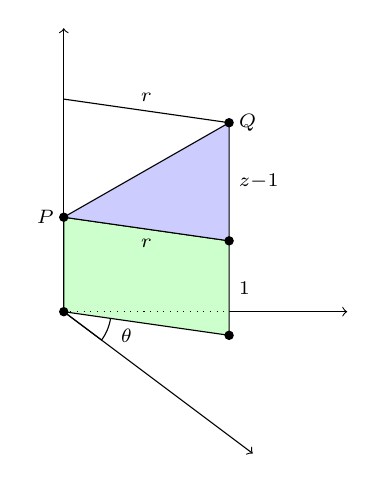
\begin{tikzpicture}[scale=3]
    \draw[->] (0,0) -- (0,1.2);
    \draw[->] (0,0) -- (1.2,0);
    \draw[->] (0,0) -- (0.8,-0.6);
    \filldraw[fill=green!20,draw=black] (0,0) -- (0.7,-0.1) -- (0.7,0.3) -- (0,0.4) -- (0,0);
    \filldraw[fill=blue!20,draw=black] (0,0.4) -- (0.7,0.3) -- (0.7,0.8) -- (0,0.4);
    \draw (0,0.9) -- (0.7,0.8);
    \draw[dotted] (0,0) -- (0.7,0);
    \draw (0,0) -- (0.16,-0.12) arc(-36.9:-8.1:0.2);
    \fill (0.0, 0.0) circle(0.02);
    \fill (0.0, 0.4) circle(0.02);
    \fill (0.7, 0.3) circle(0.02);
    \fill (0.7,-0.1) circle(0.02);
    \fill (0.7, 0.8) circle(0.02);
    \draw (0.35, 0.85) node[anchor=south] {$\ss r$};
    \draw (0.35, 0.35) node[anchor=north] {$\ss r$};
    \draw (0.70, 0.55) node[anchor=west]  {$\ss z-1$};
    \draw (0.70, 0.10) node[anchor=west]  {$\ss 1$};
    \draw (0.20,-0.10) node[anchor=west]  {$\ss \tht$};
    \draw (0.70, 0.80) node[anchor=west]  {$\ss Q$};
    \draw (0.00, 0.40) node[anchor=east]  {$\ss P$};
  \end{tikzpicture}
 \end{center}
 More algebraically, we can say that the
 rectangular coordinates of $Q$ are $(r\cos(\tht),r\sin(\tht),z)$,
 whereas the rectangular coordinates of $P$ are $(0,0,1)$.  This means
 that the vector from $P$ to $Q$ is $(r\cos(\tht),r\sin(\tht),z-1)$,
 which has length 
 \[ \sqrt{r^2\cos^2(\tht)+r^2\sin^2(\tht)+(z-1)^2} = 
     \sqrt{r^2+(z-1)^2}.
 \]
\end{solution}

\begin{exercise}
 Let $D$ be a flat-topped circular cone with cross-section as shown below:
 \begin{center}
  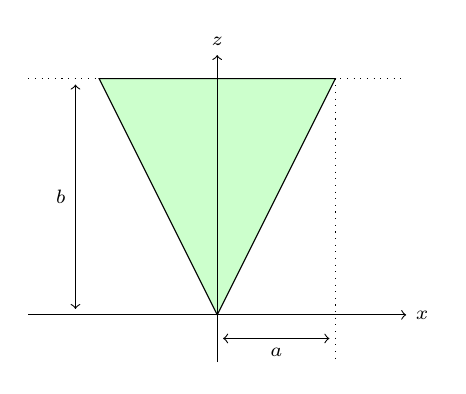
\begin{tikzpicture}[scale=1.5]
   \filldraw[draw=black,fill=green!20] (0,0) -- (1,2) -- (-1,2) -- (0,0);
   \draw[->] (-1.6,0) -- (1.6,0);
   \draw[->] (0,-0.4) -- (0,2.2);
   \draw[dotted] (-1.6,2) -- (1.6,2);
   \draw[<->] (-1.2,0.05) -- (-1.2,1.95);
   \draw[dotted] (1,2) -- (1,-0.4);
   \draw[<->] (0.05,-0.2) -- (0.95,-0.2);
   \draw ( 1.6, 0.0) node[anchor=west]  {$\ss x$};
   \draw ( 0.0, 2.2) node[anchor=south] {$\ss z$};
   \draw ( 0.5,-0.2) node[anchor=north] {$\ss a$};
   \draw (-1.2, 1.0) node[anchor=east]  {$\ss b$};
  \end{tikzpicture}
 \end{center}
 Fint the centre of mass and the moment of inertia about the $z$-axis
 (assuming that the density is $1$). 
\end{exercise}
\begin{solution}
 It is clear that $\tht$ runs from $0$ to $2\pi$, and $z$ runs from
 $0$ to $b$.  Any horizontal slice through the cone is a disk, whose
 radius depends on $z$.  At the top of the cone (where $z=b$) the
 radius is $a$, and at the bottom of the cone (where $z=0$) the radius
 is $0$.  Moreover, the radius increases uniformly in $z$, so we just
 have $r=za/b$.  This formula describes the outer wall of the cone.
 For the solid interior of the cone, we have $0\leq r\leq za/b$.  We
 can now calculate the moment of inertia about the $z$-axis.  This is
 the integral of the square of the distance from the $z$-axis, and
 that distance is just $r$, so
 \begin{align*}
  I &= \iiint_D r^2\,dV
     = \int_{\tht=0}^{2\pi} \int_{z=0}^b \int_{r=0}^{az/b}
         r^2 \, r\, dr\,dz\,d\tht \\
    &= 2\pi \int_{z=0}^b \int_{r=0}^{az/b} r^3\,dr\,dz 
     = 2\pi \int_{z=0}^b \CH{\frac{r^4}{4}}_{r=0}^{az/b}\,dz 
     = 2\pi \int_{z=0}^b \frac{a^4z^4}{4b^4} \, dz \\
    &= \frac{\pi a^4}{2b^4} \CH{\frac{z^5}{5}}_{z=0}^b
     = \frac{\pi a^4b}{10}.
 \end{align*}
 Next, it is clear by symmetry that the centre of mass must lie on the
 $z$-axis, say at $(0,0,\overline{z})$.  The general theory tells us that
 $\overline{z}=Z/V$, where $Z=\iiint_D z\,dV$ and $V=\iiint_D 1\,dV$.  These
 can be evaluated as follows:
 \begin{align*}
  Z &= \int_{\tht=0}^{2\pi} \int_{z=0}^b \int_{r=0}^{az/b}
        z \, r\, dr\, dz\, d\tht 
     = 2\pi \int_{z=0}^b \CH{\frac{z r^2}{2}}_{r=0}^{az/b} \,dz \\
    &= 2\pi \int_{z=0}^b \frac{z}{2}\left(\frac{az}{b}\right)^2\, dz
     = \frac{\pi a^2}{b^2} \int_{z=0}^b z^3 \,dz \\
    &= \frac{\pi a^2}{b^2} \,\frac{b^4}{4} = \frac{\pi a^2b^2}{4} \\
  V &= \int_{\tht=0}^{2\pi} \int_{z=0}^b \int_{r=0}^{az/b}
        r\, dr\, dz\, d\tht 
     = 2\pi \int_{z=0}^b \CH{\frac{r^2}{2}}_{r=0}^{az/b} \,dz \\
    &= \frac{\pi a^2}{b^2} \int_{z=0}^b z^2 \,dz \\
    &= \frac{\pi a^2}{b^2} \,\frac{b^3}{3} = \frac{\pi a^2b}{3} \\
  \overline{z} &= \frac{Z}{V}
          = \frac{\pi a^2b^2}{4} \, \frac{3}{\pi a^2 b}
          = \frac{3b}{4}.
 \end{align*}
\end{solution}

\begin{exercise}
 Let $D$ be the solid given by $x,y,z\geq 0$ and $x^2+y^2\leq 1$ and
 $z\leq 2$.  By rewriting everything in cylindrical coordinates,
 evaluate the integral 
 \[ I = \iiint_D x+y+z\, dV. \]
\end{exercise}
\begin{solution}
 The conditions $x,y\geq 0$ give $0\leq\tht\leq\pi/2$, and the
 condition $x^2+y^2\leq 1$ gives $0\leq r\leq 1$.  We are also given
 that $0\leq z\leq 2$.  (Geometrically, we have a quarter of a
 cylinder with radius one and height two.)  For the integrand, we have 
 \[ x+y+z = r(\cos(\tht)+\sin(\tht))+z, \]
 and $dV=r\,dr\,d\tht\,dz$.  We thus have
 \[ I = \int_{z=0}^2\int_{\tht=0}^{\pi/2}\int_{r=0}^1 
          r^2(\cos(\tht)+\sin(\tht))+zr\,dr\,d\tht\,dz.
 \]
 For the innermost integral we have
 \[ \int_{r=0}^1 r^2(\cos(\tht)+\sin(\tht))+zr\,dr = 
     \CH{\tfrac{1}{3}r^3(\cos(\tht)+\sin(\tht))+\tfrac{1}{2}zr^2}_{r=0}^1 =
     (\cos(\tht)+\sin(\tht))/3 + z/2.
 \]
 The middle integral now becomes
 \[ \int_{\tht=0}^{\pi/2} (\cos(\tht)+\sin(\tht))/3 + z/2 \,d\tht = 
    \CH{(\sin(\tht)-\cos(\tht))/3+z\tht/2}_{\tht=0}^{\pi/2} = 
    (1/3+\pi z/4) - (-1/3) = 2/3 + \pi z/4.
 \]
 Finally, the outer integral is 
 \[ I = \int_{z=0}^2 2/3 + \pi z/4\,dz = 
     \CH{2z/3 + \pi z^2/8}_{z=0}^2 = 4/3+\pi/2.
 \]
\end{solution}

\begin{exercise}
 Let $D$ be a solid cylinder, with base of radius $a$ centred at the
 origin in the $(x,y)$-plane, and height $h$.  The charge density on
 $D$ is given by $\rho(x,y,z)=x^2\sin(\pi z/h)$.  Find the total
 charge. 
\end{exercise}
\begin{solution}
 We use cylindrical polar coordinates.  The relevant limits are
 $0\leq r\leq a$ and $0\leq\tht\leq 2\pi$ and $0\leq z\leq h$.  The
 volume element $dV$ is $r\,dr\,d\tht\,dz$, and the charge density is 
 \[ \rho = x^2\sin(\pi z/h) = r^2\cos^2(\tht)\sin(\pi z/h)
     = \half r^2\sin(\pi z/h)(1+\cos(2\tht)).
 \]
 The total charge is
 \begin{align*}
  Q &= \iiint_D \rho dV 
     = \int_{z=0}^h\int_{\tht=0}^{2\pi}\int_{r=0}^a
        \half r^3\sin(\pi z/h)(1+\cos(2\tht)) \,dr\,d\tht\,dz \\
    &= \frac{1}{2}
       \left(\int_{z=0}^h\sin(\pi z/h)\,dz\right)
       \left(\int_{\tht=0}^{2\pi}(1+\cos(2\tht))\,d\tht\right)
       \left(\int_{r=0}^a r^3\,dr\right) \\
    &= \frac{1}{2}
       \CH{-\frac{h}{\pi}\cos\left(\frac{\pi z}{h}\right)}_{z=0}^h
       \CH{\tht+\half\sin(2\tht)}_{\tht=0}^{2\pi} 
       \CH{\frac{r^4}{4}}_{r=0}^a \\
    &= \frac{1}{2} .\frac{2h}{\pi} . 2\pi . \frac{a^4}{4}
     = \frac{a^4h}{2}.
 \end{align*}
\end{solution}

\begin{exercise}
 Let $P$ be the shape obtained by joining together points 
 $A,\dotsc,E$ with spherical coordinates as listed below:
 \[ \begin{array}{|c||c|c|c|c|c|}
     \hline 
          & A & B & C & D & E \\ \hline
     r    & 1 & 1 & 1 & 1 & 1 \\ \hline
     \tht & \pi/4 & 3\pi/4 & 5\pi/4 & 7\pi/4 & 0 \\ \hline
     \phi & \pi/2 & \pi/2  & \pi/2  & \pi/2  & 0 \\ \hline
    \end{array}
 \]
 Sketch $P$ and describe it geometrically.
\end{exercise}
\begin{solution}
 The points $A,\dotsc,D$ have $\phi=\pi/2$, so they are at an angle of
 $\pi/2$ to the $z$-axis, so they lie in the $xy$-plane.  They all
 have $r=1$, which means that they have distance one from the origin.
 Point $A$ is at angle $\tht=\pi/4$ to the $x$-axis, and $B$, $C$ and
 $D$ are obtained by moving round an extra $\pi/2$ each time, so they
 form a square in the $xy$-plane.  On the other hand, the point $E$
 has $\phi=0$ so it is on the $z$-axis.  The picture is as follows:
 \begin{center}
  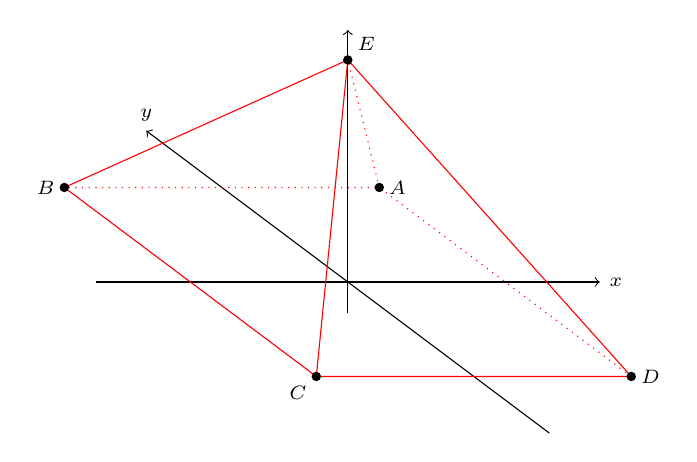
\begin{tikzpicture}[scale=2]
   \draw[->] ( 0.00,-0.20) -- ( 0.00, 1.60);
   \draw[->] (-1.60, 0.00) -- ( 1.60, 0.00);
   \draw[->] ( 1.28,-0.96) -- (-1.28, 0.96);
   \draw (1.6,0.0) node[anchor=west] {$\ss x$};
   \draw (-1.28,0.96) node[anchor=south] {$\ss y$};
   \draw[dotted,red] ( 1.80,-0.60) -- ( 0.20, 0.60) -- (-1.80, 0.60);
   \draw[red]        (-1.80, 0.60) -- (-0.20,-0.60) -- ( 1.80,-0.60);
   \draw[red]        (-1.80, 0.60) -- ( 0.00, 1.41);
   \draw[red]        (-0.20,-0.60) -- ( 0.00, 1.41);
   \draw[red]        ( 1.80,-0.60) -- ( 0.00, 1.41);
   \draw[dotted,red] ( 0.20, 0.60) -- ( 0.00, 1.41);
   \fill ( 0.20, 0.60) circle(0.03);
   \fill (-1.80, 0.60) circle(0.03);
   \fill (-0.20,-0.60) circle(0.03);
   \fill ( 1.80,-0.60) circle(0.03);
   \fill ( 0.00, 1.41) circle(0.03);
   \draw ( 0.20, 0.60) node[anchor=west]        {$\ss A$};
   \draw (-1.80, 0.60) node[anchor=east]        {$\ss B$};
   \draw (-0.20,-0.60) node[anchor=north east]  {$\ss C$};
   \draw ( 1.80,-0.60) node[anchor=west]        {$\ss D$};
   \draw ( 0.00, 1.41) node[anchor=south west]  {$\ss E$};
  \end{tikzpicture}
 \end{center}
 Thus, $P$ is a pyramid with a square base.
\end{solution}

\begin{exercise}
 Let $Q$ be the surface given in spherical coordinates by the equation
 $\tan(\phi)\sin(\tht)=1$.  Explain why $Q$ is a plane and give an
 equation for $Q$ in terms of rectangular coordinates.
\end{exercise}
\begin{solution}
 Recall that rectangular and spherical coordinates are related as
 follows:
 \begin{align*}
  x &= r \, \sin(\phi)\,\cos(\tht) \\
  y &= r \, \sin(\phi)\,\sin(\tht) \\
  z &= r \, \cos(\phi).
 \end{align*}
 From this we get 
 \[ \frac{y}{z} = 
    \frac{r\sin(\phi)\sin(\tht)}{r\cos(\phi)} = 
    \tan(\phi)\sin(\tht).
 \]
 Thus, the equation $\tan(\phi)\sin(\tht)=1$ is equivalent to $y/z=1$
 or $y=z$, which clearly describes a plane.
\end{solution}

\begin{exercise}
 Suppose that $b>a>0$, and let $D$ be the three-dimensional region
 between the spheres $x^2+y^2+z^2=a^2$ and $x^2+y^2+z^2=b^2$.
 Evaluate the integral
 \[ I = \iiint_D \frac{1}{(x^2+y^2+z^2)^{3/2}} dV. \]
\end{exercise}
\begin{solution}
 We use spherical polar coordinates, noting that $x^2+y^2+z^2=r^2$ and
 $dV=r^2\sin(\phi)\,dr\,d\tht\,d\phi$.  The integral becomes
 \begin{align*}
  I &= \int_{\phi=0}^\pi \int_{\tht=0}^{2\pi} \int_{r=a}^b 
        r^{-3}.r^2\sin(\phi)\,dr\,d\tht\,d\phi \\
    &= 2\pi \left(\int_{\phi=0}^\pi\sin(\phi)\,d\phi\right)
            \left(\int_{r=a}^b r^{-1}\,dr\right) 
     = 2\pi \CH{-\cos(\phi)}_{\phi=0}^\pi 
            \CH{\ln(r)}_{r=a}^b \\
    &= 4\pi(\ln(b)-\ln(a)) = 4\pi\ln(b/a).
 \end{align*}
\end{solution}


\begin{exercise}
 By rewriting everything in spherical polar coordinates, evaluate the
 integral 
 \[ I = \int_{x=0}^\infty \int_{y=0}^\infty \int_{z=0}^\infty 
         \exp\left(-(x^2+y^2+z^2)^{3/2}\right) dz\,dy\,dx.
 \]
\end{exercise}
\begin{solution}
 The region of integration has $x,y\geq 0$ (which means that
 $0\leq\tht\leq\pi/2$ and $z\geq 0$ (which means that
 $0\leq\phi\leq\pi/2$).  The distance $r$ from the origin can be any
 nonnegative number.  For the integrand, we have 
 \[ \exp\left(-(x^2+y^2+z^2)^{3/2}\right) = e^{-r^3}. \]
 We also have 
 \[ dz\,dy\,dx = dV = r^2\sin(\phi) dr\,d\phi\,d\tht. \]
 Thus, the integral is 
 \[ I =
      \int_{\tht=0}^{\pi/2} \int_{\phi=0}^{\pi/2} \int_{r=0}^\infty
        r^2 e^{-r^3} \sin(\phi) dr\,d\phi\,d\tht = 
      \frac{\pi}{2}
      \left(\int_{\phi=0}^{\pi/2}\sin(\phi)\,d\phi \right)
      \left(\int_{r=0}^\infty r^2 e^{-r^3}\,dr\right).
 \]
 For the $\phi$ integral we have
 \[ \int_{\phi=0}^{\pi/2}\sin(\phi)\,d\phi = 
     \CH{-\cos(\phi)}_{\phi=0}^{\pi/2} = 0 - (-1) = 1.
 \]
 For the $r$ integral we use the substitution $u=r^3$, so
 $du=3r^2\,dr$, so $dr=du/(3r^2)$.  The limits $r=0$ and $r=\infty$
 correspond to $u=0$ and $u=\infty$.  We thus get 
 \[ \int_{r=0}^\infty r^2 e^{-r^3}\,dr = 
    \int_{u=0}^\infty r^2 e^{-u} \frac{du}{3r^2} = 
    \frac{1}{3}\int_{u=0}^\infty e^{-u}\,du = 
    \frac{1}{3}\CH{-e^{-u}}_{u=0}^\infty = 1/3.
 \]
 Putting this together we get
 \[ I = \frac{\pi}{2} \tm 1 \tm \frac{1}{3} = \frac{\pi}{6}. \]
\end{solution}

\section*{Week 6 --- Vector algebra and gradients}

Unless otherwise specified, $\vr$ refers to the position vector
$\vr=(x,y,z)$, and $r=|\vr|=\sqrt{x^2+y^2+z^2}$.

\begin{exercise}
 Consider the vectors $\vp=2\vi-\vj$, $\vq=4\vi-2\vj$ and
 $\vr=2\vi+4\vj$.  Which of them are parallel to each other, and which
 of them are perpendicular to each other?
\end{exercise}
\begin{solution}
 Recall that vectors are perpendicular when their dot product is zero,
 and parallel (or antiparallel) when their cross product is zero.  We
 have 
 \begin{align*}
  \vp.\vq &= 2\tm 4+(-1)\tm(-2)=10 \\
  \vp.\vr &= 2\tm 2 + (-1)\tm 4 = 0 \\
  \vq.\vr &= 4\tm 2+(-2)\tm 4 = 0
 \end{align*}
 so $\vp$ and $\vq$ are perpendicular to $\vr$ but not to each other.
 For the cross products, we have
 \begin{align*}
  \vp\tm\vq &= \det\bsm \vi&\vj&\vk \\ 2&-1&0 \\ 4&-2&0 \esm
   = (2\tm(-2)-(-1)\tm 4)\vk = 0 \\
  \vp\tm\vr &= \det\bsm \vi&\vj&\vk \\ 2&-1&0 \\ 2&4&0 \esm
   = (2\tm 4-(-1)\tm 2)\vk = 10\vk \\
  \vq\tm\vr &= \det\bsm \vi&\vj&\vk \\ 4&-2&0 \\ 2&4&0 \esm
   = (4\tm 4-(-2)\tm 2)\vk = 20\vk,
 \end{align*}
 so $\vp$ and $\vq$ are parallel to each other, but not to $\vr$.
 More obviously, we can just observe that $\vq=2\vp$, so $\vp$ and
 $\vq$ are parallel.
\end{solution}

\begin{exercise}
 If $\va=(2,-1, 2)$, $\vb=(-1, 2, 1)$ and $\vc=(1,-2, 1)$, find the
 following quantities:
 \begin{itemize}
  \item[(a)] $|\va|$, $|\vb|$ and $|\vc|$.
  \item[(b)] $\va.\vb$, $\va.\vc$ and $\vb.\vc$.
  \item[(c)] $\va\tm\vb$,  $\va\tm\vc$ and  $\vb\tm\vc$.
  \item[(d)] The unit vector $\hva$.
  \item[(e)] The angle between $\vb$ and $\vc$.
  \item[(f)] The area of the parallelogram spanned by $\va$ and
   $\vc$.
  \item[(g)] The component of $\va$ parallel to $\vb$.
  \item[(h)] The component of $\va$ perpendicular to $\vb$.
 \end{itemize}
 Be sure to type-check your answers: do not give a vector where a
 scalar is required, or \emph{vice-versa}.
\end{exercise}
\begin{solution}
 \begin{itemize}
  \item[(a)] $|\va|=\sqrt{4+1+4}=3$; $|\vb|=\sqrt{1+4+1}=\sqrt{6}$; 
   $|\vc|=\sqrt{1+4+1}=\sqrt{6}$.
  \item[(b)]
   $\va.\vb=2\tm(-1)+(-1)\tm 2+2\tm 1=-2$;
   $\va.\vc=2\tm 1+(-1)\tm(-2)+2\tm 1=6$;
   $\vb.\vc=(-1)\tm 1+2\tm(-2)+1\tm 1=-4$.
  \item[(c)] 
   \begin{align*}
    \va\tm\vb &= \det\bsm \vi&\vj&\vk \\ 2&-1&2 \\ -1&2&1 \esm
     = (-5,-4,3) \\
    \va\tm\vc &= \det\bsm \vi&\vj&\vk \\ 2&-1&2 \\ 1&-2&1 \esm
     = (3,0,-3) \\
    \vb\tm\vc &= \det\bsm \vi&\vj&\vk \\ -1&2&1 \\ 1&-2&1 \esm
     = (4,2,0).
   \end{align*}
  \item[(d)] $\hva=\va/|\va|=\va/3=(2/3,-1/3,2/3)$.
  \item[(e)] We have 
   \[ \cos(\tht)=\frac{\vb.\vc}{|\vb||\vc|} =
       \frac{-4}{\sqrt{6}\sqrt{6}} = -\tfrac{2}{3},
   \]
   so $\tht=\arccos(-2/3)$, which is $2.3$ radians or $132$ degrees.
  \item[(f)] The area is
   $|\va\tm\vc|=\sqrt{3^2+0^2+(-3)^2}=\sqrt{18}=3\sqrt{2}\simeq 4.24$.
  \item[(g)] The parallel component is 
   \[ \va_{||} = \frac{\va.\vb}{\vb.\vb} \vb
       = \frac{-2}{6}(-1,2,1) = 
        (\tfrac{1}{3},-\tfrac{2}{3},-\tfrac{1}{3}).
   \]
  \item[(h)] The perpendicular component is 
   \[ \va_{\perp} = \va - \va_{||} =
      (2,-1,2)-(\tfrac{1}{3},-\tfrac{2}{3},-\tfrac{1}{3}) =
      (\tfrac{5}{3},-\tfrac{1}{3},\tfrac{7}{3}).
   \]
 \end{itemize}
\end{solution}

\begin{exercise}
 Consider vectors $\va=(u,v,w)$ and $\vb=(x,y,z)$.  Give formulae for 
 $\va.\vb$ and $\va\tm\vb$ and $|\va\tm\vb|^2$.  Verify by direct
 expansion that 
 \[ (\va.\vb)^2+|\va\tm\vb|^2=|\va|^2|\vb|^2. \]
\end{exercise}
\begin{solution}
 \begin{align*}
  \va.\vb &= ux+vy+wz \\
  (\va.\vb)^2 &= u^2x^2+v^2y^2+w^2z^2+2uvxy+2uwxz+2vwyz \\
  \va\tm\vb &= (vz-wy,\;wx-uz,\;uy-vx) \\
  |\va\tm\vb|^2 &= (vz-wy)^2+(wx-uz)^2+(uy-vx)^2 \\
   &= v^2z^2-2vwyz+w^2y^2 +
      w^2x^2-2uwxz+u^2z^2 +
      u^2y^2-2uvxy+v^2x^2. \\
  (\va.\vb)^2+|\va\tm\vb|^2 
   &= u^2x^2+v^2y^2+w^2z^2+
      v^2z^2+w^2y^2 +
      w^2x^2+u^2z^2 +
      u^2y^2+v^2x^2 \\
   &= (u^2+v^2+w^2)(x^2+y^2+z^2) \\
   &= |\va|^2|\vb|^2.
 \end{align*}
 Note that if we believe the formulae $\va.\vb=|\va||\vb|\cos(\tht)$
 and $|\va\tm\vb|=|\va||\vb|\sin(\tht)$ then we have a simpler
 argument:
 \[ (\va.\vb)^2+|\va\tm\vb|^2 = 
     |\va|^2|\vb|^2\cos^2(\tht) + |\va|^2|\vb|^2\sin^2(\tht) =
      |\va|^2|\vb|^2. 
 \]
 However, this is not really a satisfactory argument, because the more
 complicated calculation given above is required in order to prove the
 formula $|\va\tm\vb|=|\va||\vb|\sin(\tht)$ in the first place.
\end{solution}

\begin{exercise}
 Find $\grad(f)$ for the following functions 
 \begin{itemize}
  \item[(a)] $f=x^2y+y^2z+z^2x$
  \item[(b)] $f=\sin(r)/r$
  \item[(c)] $f=e^{-x^2-y^2}+z$.
 \end{itemize}
\end{exercise}
\begin{solution}
 \begin{itemize}
  \item[(a)] $\grad(f)=(f_x,f_y,f_z)=(2xy+z^2,2yz+x^2,2zx+y^2)$.
  \item[(b)] Recall that 
   \[ r_x = \frac{\partial r}{\partial x} = \ddx(x^2+y^2+z^2)^{\half} =
       \half(x^2+y^2+z^2)^{-\half}.2x = x/r,
   \]
   and similarly $r_y=y/r$ and $r_z=z/r$.  We also have
   \[ \frac{df}{dr} = \frac{\cos(r)r-\sin(r)}{r^2}, \]
   and 
   \[ f_x = \frac{\partial f}{\partial x} =
       \frac{df}{dr}\,\frac{\partial r}{\partial x} = 
       \frac{\cos(r)r-\sin(r)}{r^2}\,\frac{x}{r} = 
        \frac{\cos(r)r-\sin(r)}{r^3}\,x.
   \]
   We can find $f_y$ and $f_z$ in the same way, giving
   \[ \grad(f) = (f_x,f_y,f_z) =
       \frac{\cos(r)r-\sin(r)}{r^3} (x,y,z).
   \]
  \item[(c)] In this case we have
   $\grad(f)=(-2xe^{-x^2-y^2},-2ye^{-x^2-y^2},1)$.
 \end{itemize}
\end{solution}

\begin{exercise}
 If $f=x^2yz^3$ and $\vn=(\frac{1}{3},\frac{2}{3},\frac{2}{3})$, find
 the directional derivative $\vn.\nabla(f)$.
\end{exercise}
\begin{solution}
 $\nabla(f)=(2xyz^3,x^2z^3,3x^2yz^2)$, so 
 \[ \vn.\nabla(f) =
     \frac{2}{3}xyz^3 + \frac{2}{3}x^2z^3 + 2x^2yz^2.
 \]
\end{solution}

\begin{exercise}
 The scalar field $f$ is given by $f=x\sin(xy)+z\cos(xy)$.
 Find the component of $\grad(f)$ in parallel to $(-1,1,-1)$ at the point
 $(\pi/2,2,0)$.
\end{exercise}
\begin{solution}
 Here 
 \[ \nabla(f)=(\sin(xy)+xy\cos(xy)-yz\sin(xy),
               x^2\cos(xy)-xz\sin(xy),\cos(xy)).
 \]
 At the point $(x,y,z)=(\pi/2,2,0)$ we have $xy=\pi$ so $\sin(xy)=0$ and
 $\cos(xy)=-1$ so 
 \[ \nabla(f) = (-\pi,-\pi^2/4,-1). \]
 Now put $\vm=(-1,1,-1)$, so
 $\nabla(f).\vm=\pi-\pi^2/4+1=\frac{1}{4}(4+4\pi-\pi^2)$ and
 $\vm.\vm=3$.  The component of $\nabla(f)$ parallel to the $\vm$ is
 given by  
 \[ \nabla(f)_{||} = \frac{\nabla(f).\vm}{\vm.\vm} \vm =
     \frac{4+4\pi-\pi^2}{12} (-1,1,-1).
 \]
\end{solution}

\begin{exercise}
 Put $f=x^2-z^2$ and $g=2xz+y^2$.  Show that $\nabla(f)$ is always
 perpendicular to $\nabla(g)$.
\end{exercise}
\begin{solution}
 \begin{align*}
  \nabla(f) &= (2x,0,-2z) \\
  \nabla(g) &= (2z,2y,2x) \\
  \nabla(f) . \nabla(g) &= 
    (2x)\tm(2z) + 0\tm 2y + (-2z)\tm(2x) = 4xz-4xz = 0.
 \end{align*}
 As $\nabla(f).\nabla(g)=0$ for all $x$, $y$ and $z$, we see that
 $\nabla(f)$ and $\nabla(g)$ are perpendicular at all points.
\end{solution}

\section*{Week 7 --- Div and curl }

\begin{exercise}
 Find $\nabla.\vu$ and $\nabla\tm\vu$ for the following vector fields:
 \[ \text{(a):}\qquad \vu=(xy,yz,0) \hspace{5em}
    \text{(b):}\qquad \vu=(z,x,y).
 \]
\end{exercise}
\begin{solution}
 \begin{itemize}
  \item[(a)] $\nabla.\vu=\ddx(xy)+\ddy(yz)+\ddz(0)=y+z$ and 
   \[ \nabla\tm\vu =
       \det\bsm \vi & \vj & \vk \\ \ddx & \ddy & \ddz \\ 
                xy & yz & 0 \esm = 
        \left(\ddy(0)-\ddz(yz),\ddz(xy)-\ddx(yz),\ddx(yz)-\ddy(xy)\right)
         = (-y,0,-x).
   \]
  \item[(b)] $\nabla.\vu=\ddx(z)+\ddy(x)+\ddz(y)=0+0+0=0$ and 
   \[ \nabla\tm\vu =
       \det\bsm \vi & \vj & \vk \\ \ddx & \ddy & \ddz \\ 
                z & x & y \esm = 
        \left(\ddy(y)-\ddz(x),\ddz(z)-\ddx(y),\ddx(x)-\ddy(z)\right)
         = (1,1,1).
   \]
 \end{itemize}
\end{solution}

\begin{exercise}
 Consider a vector field of the form $\vu=f(r)\vr$, where $f$ is a
 function of $r$ only.  Show that $\nabla.\vu=3\,f(r)+r\,f'(r)$.  Show
 that if $\nabla.\vu=0$, then $f(r)=c/r^3$ for some constant $c$.

 [\textbf{Hint:} remember the chain rule
 $\ddx f(r)=f'(r)\frac{\partial r}{\partial x}$.]
\end{exercise}
\begin{solution}
 We have $\vu=(f(r)x,f(r)y,f(r)z)$, so 
 \[ \nabla.\vu = \ddx(f(r)x) + \ddy(f(r)y) + \ddz(f(r)z). \]
 Using the product rule, the chain rule, and the the standard fact
 that $\partial r/\partial x=x/r$, we get 
 \[ \ddx(f(r)x) = f(r)+x\ddx f(r) =
     f(r)+x\,f'(r) \frac{\partial r}{\partial x} = 
      f(r)+x^2\,f'(r)/r.
 \]
 We can treat the other two terms in the same way to get 
 \begin{align*}
  \nabla.\vu &=
   \ddx(f(r)x) + \ddy(f(r)y) + \ddz(f(r)z) \\
  &= f(r) + \frac{x^2}{r}f'(r) + 
     f(r) + \frac{y^2}{r}f'(r) + 
     f(r) + \frac{z^2}{r}f'(r) 
   = 3\,f(r) + \frac{x^2+y^2+z^2}{r}\, f'(r) 
   = 3\,f(r) + \frac{r^2}{r}\,f'(r) \\
  &= 3\,f(r)+r\,f'(r).
 \end{align*}
 Now suppose that $\nabla.\vu=0$, so $3 f(r)+r\,f'(r)=0$.  Put
 $g(r)=r^3\,f(r)$, so 
 \[ g'(r) = 3r^2\,f(r)+r^3\,f'(r) = 
     r^2(3 f(r)+r\,f'(r)) = 0.
 \]
 This means that $g(r)$ is a constant, say $c$.  As
 $c=g(r)=r^3\,f(r)$, it follows that $f(r)=c/r^3$.  
\end{solution}

\begin{exercise}
 Find constants $a$, $b$ and $c$ such that the vector field
 \[ \vv = (x+2y+az,\; bx-3y-z,\; 4x+cy+2z) \]
 satisfies $\curl(\vv)=0$.  For these values of $a$, $b$ and $c$, find
 a potential function $f$ with $\grad(f)=\vv$.
\end{exercise}
\begin{solution}
 We have 
 \[ \curl(\vv) = 
     \det\bbm \vi & \vj & \vk \\
      \ddx & \ddy & \ddz \\
      x+2y+az & bx-3y-z & 4x+cy+2z \ebm = 
       (c-(-1),a-4,b-2).
 \]
 For this to be zero we must have $a=4$ and $b=2$ and $c=-1$, so 
 \[ \vv = (x+2y+4z,\; 2x-3y-z,\; 4x-y+2z). \]
 We want this to be equal to $\grad(f)$, which means that
 \begin{align*}
  f_x &= x+2y+4z \tag{A} \\
  f_y &= 2x-3y-z \tag{B} \\
  f_z &= 4x-y+2z \tag{C} 
 \end{align*}
 By integrating~(A), we see that 
 \[ f=\int x+2y+4z\,dx = \half x^2 + 2xy + 4xz + p, \tag{D} \]
 where $p$ is constant with respect to $x$, so $p$ depends only on $y$
 and $z$.  We now differentiate~(D) with respect to $y$ to get
 \[ f_y = 2x+p_y. \tag{E}\]
 On the other hand, equation~(B) says that $f_y=2x-3y-z$.  By
 comparing~(B) and~(E) we see that $p_y=-3y-z$.  We can now integrate
 with respect to $y$ to get 
 \[ p = -\tfrac{3}{2}y^2-yz+q, \tag{F} \]
 where $q$ is constant with respect to both $x$ and $y$, so it depends
 only on $z$.  We can substitute~(F) in~(D) to get
 \[ f = \half x^2 + 2xy + 4xz -\tfrac{3}{2}y^2-yz + q. \tag{G} \]
 We can differentiate~(G) with respect to $z$ to get 
 \[ f_z = 4x - y + q_z. \tag{H} \]
 On the other hand, equation~(C) says that $f_z=4x-y+2z$.  By
 comparing~(C) and~(H) we see that $q_z=2z$, so $q=z^2$ (plus a
 constant, which we can take to be zero).  We can substitute this
 in~(G) to get
 \[ f = \half x^2 + 2xy + 4xz -\tfrac{3}{2}y^2-yz + z^2. \]
 As a final check, we can calculate directly that
 \begin{align*}
  f_x &= x+2y+4z \\
  f_y &= 2x-3y-z \\
  f_z &= 4x-y+2z
 \end{align*}
 as required.
\end{solution}

\begin{exercise}
 If $r=\sqrt{x^2+y^2+z^2}$, show that $\nabla^2(r^n)=n(n+1)r^{n-2}$.
\end{exercise}
\begin{solution}
 We have seen before that $r_x=x/r$, which implies that
 \[ (r^n)_x = n\,r^{n-1} r_x = n\, r^{n-1} x/r = n\,r^{n-2} x.
      \tag{A}
 \]
 In the same way, we have
 \[ (r^{n-2})_x = (n-2) r^{n-4} x. \]
 We can differentiate~(A) once more using the product rule to get
 \begin{align*}
  (r^n)_{xx}
   &= (n\,r^{n-2}x)_x
    = n\,(r^{n-2})_x\,x + n\,r^{n-2} \\
   &= n((n-2) r^{n-4}\,x)\,x + n r^{n-2} 
    = (n^2-2n) r^{n-4}\,x^2 + n r^{n-2}.
 \end{align*}
 In the same way, we have 
 \begin{align*}
  (r^n)_{yy} &= (n^2-2n) r^{n-4}\,y^2 + n r^{n-2} \\
  (r^n)_{zz} &= (n^2-2n) r^{n-4}\,z^2 + n r^{n-2}.
 \end{align*}
 Adding these together, we get
 \begin{align*}
  \nabla^2(r^n) 
   &= (r^n)_{xx} + (r^n)_{yy} + (r^n)_{zz} \\
   &= (n^2-2n) r^{n-4}\,x^2 + n r^{n-2} + 
      (n^2-2n) r^{n-4}\,y^2 + n r^{n-2} + 
      (n^2-2n) r^{n-4}\,z^2 + n r^{n-2} \\
   &= (n^2-2n) r^{n-4}(x^2+y^2+z^2) + 3nr^{n-2} 
    = (n^2-2n) r^{n-4}\,r^2 + 3nr^{n-2} \\
   &= (n^2+n) r^{n-2} = n(n+1)r^{n-2}
 \end{align*}
 as claimed.
\end{solution}

\begin{exercise}
 Let $\Omega$ be a scalar field, and let $\vF$ be a vector field.
 Show that 
 \begin{itemize}
  \item[(a)] $\curl(\Omega\vF)=\Omega\,\curl(\vF)-\vF\tm\grad(\Omega)$
  \item[(b)] $\curl(\grad(\Omega))=0$.
 \end{itemize}
 Rewrite these identities in $\nabla$ notation.
\end{exercise}
\begin{solution}
 Write $\vF=(P,Q,R)$, so $\Omega\vF=(\Omega P,\Omega Q,\Omega R)$.  We
 have 
 \begin{align*}
  \curl(\Omega\vF)
   &= 
   \det\bbm \vi & \vj & \vk \\
    \ddx & \ddy & \ddz \\
    \Omega P & \Omega Q & \Omega R
   \ebm
   = ((\Omega R)_y-(\Omega Q)_z,\;
      (\Omega P)_z-(\Omega R)_x,\;
      (\Omega Q)_x-(\Omega P)_y) \\
   &= (\Omega_y R + \Omega R_y - \Omega_z Q - \Omega Q_z,\;
       \Omega_z P + \Omega P_z - \Omega_x R - \Omega R_x,\;
       \Omega_x Q + \Omega Q_x - \Omega_y P - \Omega P_y) \\
   &= \Omega(R_y-Q_z,\; P_z-R_x,\; Q_x-P_y) +
      (\Omega_y R - \Omega_z Q,\;
       \Omega_z P - \Omega_x R,\;
       \Omega_x Q - \Omega_y P) \tag{A} \\
   \Omega\,\curl(\vF) &= 
    \Omega\,\det\bbm \vi & \vj & \vk \\
     \ddx & \ddy & \ddz \\
     P & Q & R \ebm =
     \Omega(R_y-Q_z,\;P_z-R_x,\;Q_x-P_y) \tag{B}\\
   \vF\tm\grad(\Omega) &= 
    \det\bbm
     \vi      & \vj      & \vk  \\
     P        & Q        & R    \\
     \Omega_x & \Omega_y & \Omega_z
    \ebm 
     = (\Omega_z Q-\Omega_y R,\;
        \Omega_x R-\Omega_z P,\;
        \Omega_y P-\Omega_x Q) \tag{C}
 \end{align*}
 Combining~(A), (B) and~(C) makes it clear that 
 $\curl(\Omega\vF)=\Omega\,\curl(\vF)-\vF\tm\grad(\Omega)$.  In
 $\nabla$ notation, this becomes
 $\nabla\tm(\Omega\vF)=\Omega\,\nabla\tm\vF-\vF\tm\nabla(\Omega)$.

 Next, we have
 \begin{align*}
  \grad(\Omega) &= (\Omega_x,\;\Omega_y,\;\Omega_z) \\
  \curl(\grad(\Omega)) &= 
   \det\bbm 
    \vi      & \vj      & \vk  \\
    \ddx     & \ddy     & \ddz \\
    \Omega_x & \Omega_y & \Omega_z
   \ebm 
   = (\Omega_{zy} - \Omega_{yz},
      \Omega_{xz} - \Omega_{zx},
      \Omega_{yx} - \Omega_{xy}) 
   = (0,0,0).
 \end{align*}
 In $\nabla$ notation, this says that $\nabla\tm(\nabla(\Omega))=0$.
\end{solution}

\begin{exercise}
 Let $\vH$ be a vector field that can be expressed as
 $\vH=f\,\grad(g)$ for some scalar fields $f$ and $g$.  Show that
 $\vH$ is perpendicular to $\curl(\vH)$ at every point.

 \noindent{[\textbf{Hint:} use the previous question.]}

 \medskip

 Now consider the vector field $\vH=x^2y\,\vr$ (where $\vr=(x,y,z)$ as
 usual).  Find scalar fields $f$ and $g$ such that $\vH=f\,\grad(g)$.  
 Calculate $\curl(\vH)$ and check directly that it is perpendicular to
 $\vH$.  
\end{exercise}
\begin{solution}
 Using the previous question (with $\Omega=f$ and $\vF=\grad(g)$) we
 see that 
 \[ \curl(\vH) = \curl(f\,\grad(g))
    = f\curl(\grad(g)) - \grad(g)\tm\grad(f).
 \]
 As $\curl(\grad(g))=0$, this simplifies to
 $\curl(\vH)=-\grad(g)\tm\grad(f)=\grad(f)\tm\grad(g)$.  It is a
 general rule that $\va\tm\vb$ is always perpendicular to $\va$ and to
 $\vb$, so $\curl(\vH)$ is perpendicular to $\grad(g)$.  Moreover,
 $\vH$ is just the scalar $f$ times the vector $\grad(g)$, so it has
 the same direction as $\grad(g)$, so it is also perpendicular to
 $\vH$.  

 Now consider the case 
 \[ \vH = x^2y\vr = (x^3y,\;x^2y^2,\;x^2yz). \]
 We know that $\grad(r)=(x/r,y/r,z/r)=\vr/r$, so 
 \[ \vH = x^2yr\;\vr/r = x^2yr\,\grad(r). \]
 Thus, if we take $f=x^2yr$ and $g=r$ then $\vH=f\,\grad(g)$.  A
 different, but equally valid, solution is to take $f=x^2y$ and
 $g=r^2/2=(x^2+y^2+z^2)/2$.  

 The first part of the question now tells us that $\curl(\vH)$
 should be perpendicular to $\vH$.  We can check this directly as
 follows.  We have
 \[ \curl(\vH) = 
     \det\bbm \vi & \vj & \vk \\ \ddx & \ddy & \ddz \\
      x^3y & x^2y^2 & x^2yz \ebm =
      (x^2z-0,\;0-2xyz,\;2xy^2-x^3) =
       (x^2z,\;-2xyz,\;2xy^2-x^3),
 \]
 so 
 \[ \vH . \curl(\vH) =
     (x^3y,\;x^2y^2,\;x^2yz) . (x^2z,\;-2xyz,\;2xy^2-x^3) =
     x^5yz-2x^3y^3z+2x^3y^3z-x^5yz = 0,
 \]
 which means that $\vH$ and $\curl(\vH)$ are perpendicular.
\end{solution}

\begin{exercise}
 For the vector field $\vA=(x^2y,\;y^2z,\;z^2x)$, calculate
 \begin{itemize}
  \item[(a)] $\nabla.\vA$
  \item[(b)] $\nabla(\nabla.\vA)$
  \item[(c)] $\nabla\tm\vA$
  \item[(d)] $\nabla\tm(\nabla\tm\vA)$
  \item[(e)] $\nabla^2(\vA)$.
 \end{itemize}
 Verify the identity
 $\nabla^2(\vA)=\nabla(\nabla.\vA)-\nabla\tm(\nabla\tm\vA)$ in this
 case. 
\end{exercise}
\begin{solution}
 \begin{itemize}
  \item[(a)]
   $\nabla.\vA=\ddx(x^2y)+\ddy(y^2z)+\ddz(z^2x)=2xy+2yz+2zx$.
  \item[(b)] $\nabla(\nabla.\vA)=\nabla(2xy+2yz+2zx)=
   (2y+2z,\;2z+2x,\;2x+2y)$.
  \item[(c)] $\nabla\tm\vA=\det\bsm \vi&\vj&\vk \\ \ddx&\ddy&\ddz \\
   x^2y& y^2z& z^2x\esm = (0-y^2,\;0-z^2,\;0-x^2)=(-y^2,-z^2,-x^2)$.
  \item[(d)] $\nabla\tm(\nabla\tm\vA)=\det\bsm \vi&\vj&\vk \\ \ddx&\ddy&\ddz \\
   -y^2& -z^2& -x^2 \esm=(0-(-2z),\;0-(-2x),\;0-(-2y))=(2z,2x,2y)$.
  \item[(e)] Note that $\nabla(x^2y)=(2xy,x^2,0)$, so 
   \[ \nabla^2(x^2y) = \nabla.(2xy,x^2,0) = 
       \ddx(2xy) + \ddy(x^2) +\ddz(0) = 2y.
   \]
   In the same way, we have $\nabla^2(y^2z)=2z$ and
   $\nabla^2(z^2x)=2x$, so 
   \[ \nabla^2(\vA)=(\nabla^2(x^2y),\nabla^2(y^2z),\nabla^2(z^2x)))=
       (2y,2z,2x).
   \]
 \end{itemize}
 We now see that 
 \[ \nabla(\nabla.\vA)-\nabla\tm(\nabla\tm(\vA)) =
     (2y+2z,\;2z+2x,\;2x+2y) - (2z,2x,2y) = 
      (2y,2z,2x) = \nabla^2(\vA)
 \]
 as claimed.
\end{solution}

\begin{exercise}
 Show that for any vector fields $\vu=(p,\;q,\;r)$ and
 $\vv=(f,\;g,\;h)$ we have 
 \[ \nabla.(\vu\tm\vv)=
     (\nabla\tm\vu).\vv - (\nabla\tm\vv).\vu.
 \]
\end{exercise}
\begin{solution}
 \begin{align*}
  \nabla\tm\vu =\;& (r_y-q_z,\;p_z-r_x,\;q_x-p_y) \\
  \nabla\tm\vv =\;& (h_y-g_z,\;f_z-h_x,\;g_x-f_y) \\
  \vu\tm\vv =\;& (qh-rg,\;rf-ph,\;pg-qf) \\
  \nabla.(\vu\tm\vv) =\;& 
   (qh-rg)_x\;+\;(rf-ph)_y\;+\;(pg-qf)_z \\
   \\
  =\;& \BLUE{q_xh}\MAGENTA{+qh_x}\OLG{-r_xg}\RAWSIENNA{-rg_x}+ \\
     & \RED{r_yf}\RAWSIENNA{+rf_y}\BLUE{-p_yh}\CYAN{-ph_y}+ \\
     & \OLG{p_zg}\CYAN{+pg_z}\RED{-q_zf}\MAGENTA{-qf_z} \\
  =\;& \RED{(r_y-q_z)f}+\OLG{(p_z-r_x)g}+\BLUE{(q_x-p_y)h}+ \\
     & \CYAN{p(g_z-h_y)}+\MAGENTA{q(h_x-f_z)}+\RAWSIENNA{r(f_y-g_x)} \\
  =\;& (r_y-q_z,\;p_z-r_x,\;q_x-p_y).(f,\;g,\;h) - \\
     & (p,\;q,\;r).(h_y-g_z,\;f_z-h_x,\;g_x-f_y) \\
  =\;& (\nabla\tm\vu).\vv - (\nabla\tm\vv).\vu.
 \end{align*}
\end{solution}

\section*{Week 8 --- Polar fields and line integrals}

There are formulae for div, grad and curl in polar coordinates on the
back of this sheet.

\begin{exercise}
 Let $\vu$ be the vector field given in spherical polar coordinates by
 \[ \vu = r^2\cos(\zen) \ve_r + r^{-1}\ve_{\zen} +
            (r\,\sin(\zen))^{-1}\ve_{\azi}
 \]
 Find $\dv(\vu)$ and $\curl(\vu)$.
\end{exercise}
\begin{solution}
 The general formulae are 
 \begin{align*}
  \dv(m\ve_r+p\ve_\zen+q\ve_\azi)
     &= r^{-2}(r^2m)_r + (r\sin(\zen))^{-1}(\sin(\zen)p)_\zen + 
         (r\sin(\zen))^{-1}q_\azi \\
  \curl(m\ve_r+p\ve_\zen+q\ve_\azi)
     &= \frac{1}{r^2\sin(\zen)} \det\bbm
          \ve_r & r\ve_\zen & r\sin(\zen)\ve_\azi \\
          \ddr  & \ddp      & \ddt  \\
          m     & rp        & r\sin(\zen)q \ebm.
 \end{align*}
 In the present case we have $m=r^2\cos(\zen)$ and $p=r^{-1}$ and
 $q=(r\,\sin(\zen))^{-1}$.  This gives
 \begin{align*}
  r^{-2}(r^2m)_r
   &= r^{-2}(r^4\cos(\zen))_r
    = r^{-2}\tm 4r^3\cos(\zen)
    = 4r\cos(\zen) \\
  (r\sin(\zen))^{-1}(\sin(\zen)p)_\zen
   &= (r\sin(\zen))^{-1}(r^{-1}\sin(\zen))_\zen
    = \frac{r^{-1}\cos(\zen)}{r\sin(\zen)}
    = r^{-2}\cot(\zen) \\
  (r\sin(\zen))^{-1}q_\azi 
   &= 0 \\
  \dv(\vu) &= 4r\cos(\zen) + r^{-2}\cot(\zen)
 \end{align*}
 Next, we have
 \[ \curl(\vu) = 
      \frac{1}{r^2\sin(\zen)} \det\bbm
          \ve_r & r\ve_\zen & r\sin(\zen)\ve_\azi \\
          \ddr  & \ddp      & \ddt  \\
          r^2\cos(\zen) & 1 & 1 \ebm.
 \]
 The relevant $2\tm 2$ determinants are 
 \begin{align*}
  \det\bbm \ddp & \ddt \\ 1 & 1 \ebm 
   &= 0 - 0 = 0 \\
  \det\bbm \ddr & \ddt \\ r^2\cos(\zen) & 1 \ebm 
   &= 0 - 0 = 0 \\
  \det\bbm \ddr & \ddp \\ r^2\cos(\zen) & 1 \ebm 
   &= 0 - (-r^2\sin(\zen)) = r^2\sin(\zen).
 \end{align*}
 This gives
 \[ \curl(\vu) =
     \frac{1}{r^2\sin(\zen)}\left(
      0 \ve_r - 0 (r\ve_\zen) + r^2\sin(\zen)(r\sin(\zen)\ve_\azi)
     \right) = r\,\sin(\zen)\ve_\azi.
 \]
\end{solution}

\begin{exercise}
 Let $\vu$ be the vector field given in cylindrical polar coordinates
 by 
 \[ \vu = r\cos(\azi) \ve_r + r\sin(\azi)\ve_\azi + \ve_z. \]
 Find $\dv(\vu)$ and $\curl(\vu)$.
\end{exercise}
\begin{solution}
 The general formulae are
 \begin{align*}
  \dv(m\ve_r+p\ve_\azi+q\ve_z)
   &= r^{-1}m + m_r + r^{-1}p_\azi + q_z 
    = r^{-1}(rm)_r + r^{-1}p_\azi + q_z \\
  \curl(m\ve_r+p\ve_\azi+q\ve_z)
   &= \frac{1}{r} \det\bbm
        \ve_r & r\ve_\azi & \ve_z \\
        \ddr  & \ddt      & \ddz  \\
        m     & rp        & q \ebm.
 \end{align*}
 In the present case we have $m=r\cos(\azi)$ and $p=r\sin(\azi)$ and
 $q=1$.  This gives
 \begin{align*}
  r^{-1}m &= \cos(\azi) \\
  m_r &= \cos(\azi) \\
  r^{-1}p_\azi &= \cos(\azi) \\
  q_z &= 0 \\
  \dv(\vu) &= 3\cos(\azi) 
 \end{align*}
 Next, we have 
 \[ \curl(\vu) = 
       \frac{1}{r} \det\bbm
         \ve_r & r\ve_\azi & \ve_z \\
         \ddr  & \ddt      & \ddz  \\
         r\cos(\azi) & r^2\sin(\azi) & 1 \ebm.
 \]
 The relevant $2\tm 2$ determinants are
 \begin{align*}
  \det\bbm \ddt & \ddz \\ r^2\sin(\azi) & 1 \ebm 
   &= 0-0 = 0 \\
  \det\bbm \ddr & \ddz \\ r\cos(\azi) & 1 \ebm 
   &= 0-0 = 0 \\
  \det\bbm \ddr & \ddt \\ r\cos(\azi) & r^2\sin(\azi) \ebm 
   &= 2r\sin(\azi)-(-r\sin(\azi)) = 3r\sin(\azi)
 \end{align*}
 so 
 \[ \curl(\vu) = 
     \frac{1}{r}\left(
      0\ve_r - 0(r\ve_\tht) + 3r\sin(\azi)\ve_z
     \right) = 3\sin(\azi)\ve_z.
 \] 
\end{solution}

\begin{exercise}
 Consider the vector field $\vu=r^{-2}\vr$, where $\vr=(x,y,z)$ and
 $r=|\vr|$.  Show that $\curl(\vu)=0$ and $\dv(\vu)=r^{-2}$.    
\end{exercise}
\begin{solution}
 One approach is to use spherical polar coordinates.  Recall that
 $\vr=r\,\ve_r$, so we can write $\vu=r^{-2}r\ve_r=r^{-1}\ve_r$.  
 The general formulae are 
 \begin{align*}
  \dv(m\ve_r+p\ve_\zen+q\ve_\azi)
     &= r^{-2}(r^2m)_r + (r\sin(\zen))^{-1}(\sin(\zen)p)_\zen + 
         (r\sin(\zen))^{-1}q_\azi \\
  \curl(m\ve_r+p\ve_\zen+q\ve_\azi)
     &= \frac{1}{r^2\sin(\zen)} \det\bbm
          \ve_r & r\ve_\zen & r\sin(\zen)\ve_\azi \\
          \ddr  & \ddp      & \ddt  \\
          m     & rp        & r\sin(\zen)q \ebm.
 \end{align*}
 In the present case we have $m=r^{-1}$ and $p=q=0$, so 
 \[ \dv(\vu) = r^{-2}(r^2m)_r = r^{-2}(r)_r = r^{-2}. \]
 We also have
 \[ \curl(\vu) 
     = \frac{1}{r^2\sin(\zen)} \det\bbm
          \ve_r & r\ve_\zen & r\sin(\zen)\ve_\azi \\
          \ddr  & \ddp      & \ddt  \\
          r^{-1} & 0        & 0 \ebm
     = 0 - 0 + 0 = 0.
 \]
 Alternatively, we could use rectangular coordinates.  We have 
 \[ \vu = \vr/r^2 =
     \left(\frac{x}{x^2+y^2+z^2},\;
           \frac{y}{x^2+y^2+z^2},\;
           \frac{z}{x^2+y^2+z^2}\right)
 \]
 The first term in the divergence is
 \[ \ddx\left(\frac{x}{x^2+y^2+z^2}\right) = 
     \frac{1.(x^2+y^2+z^2)-x.2x}{(x^2+y^2+z^2)^2} =
       r^{-2} - 2x^2r^{-4}.
 \]
 Similarly, the second term is $r^{-2}-2y^2r^{-4}$ and the third term
 is $r^{-2}-2z^2r^{-4}$.  Adding these together, we get
 \[ \dv(\vu) = 
     3r^{-2}-2(x^2+y^2+z^2)r^{-4} = 3r^{-2}-2r^2r^{-4} = r^{-2}.
 \]
 For the curl we note that 
 \[ \ddy\left(\frac{z}{r^2}\right) = 
    \ddy\left(\frac{z}{x^2+y^2+z^2}\right) =
    \frac{-2yz}{(x^2+y^2+z^2)^4} = -2yz/r^4
 \]
 and similarly $\ddx(z/r^2)=-2xz/r^4$ and so on.  This means that 
 \[ \curl(\vu) = 
   \det\bbm \vi & \vj & \vk \\
            \ddx & \ddy & \ddz \\
            x/r^2 & y/r^2 & z/r^2 \ebm 
   = (-yz/r^2+yz/r^2,\;-xz/r^2+xz/r^2,\;-xy/r^2+xy/r^2)
   = (0,0,0).
 \]
\end{solution}

\begin{exercise}
 Let $r$ denote $\sqrt{x^2+y^2}$ as in cylindrical polar coordinates.
 Use the formula for $\nabla^2$ in those coordinates to show that
 $\nabla^2(r^2+z^2)=6$. 
\end{exercise}
\begin{solution}
 The general rule is
 \[ \nabla^2(f) = r^{-1}f_r + f_{rr} + r^{-2}f_{\azi\azi} + f_{zz}.
 \] 
 In the present case we have $f=r^2+z^2$ so 
 \begin{align*}
  f_r    &= 2r & f_\azi       &= 0 & f_z    &= 2z \\
  f_{rr} &= 2  & f_{\azi\azi} &= 0 & f_{zz} &= 2
 \end{align*}
 so
 \[ \nabla^2(f) = r^{-1}.(2r) + 2 + 0 + 2 = 6. \]
\end{solution}

\begin{exercise}
 Evaluate $\int_Cx^2\,|d\vr|$, where $C$ is the circle of radius $a$
 centred at the origin.
\end{exercise}
\begin{solution}
 We can parametrise $C$ as $\vr=(a\cos(t),a\sin(t))$ (for
 $0\leq t\leq 2\pi$).  This gives
 \begin{align*}
  d\vr &= (-a\sin(t),a\cos(t))\,dt \\
  |d\vr| &= \sqrt{(a\sin(t))^2+(a\cos(t))^2} dt
          = a\sqrt{\sin^2(t)+\cos^2(t)}\,dt = a\,dt \\
  x^2 &= (a\cos(t))^2 = a^2\,\cos^2(t) \\
  \int_C x^2\,|d\vr| &= 
   \int_{t=0}^{2\pi} a^2\cos^2(t)\,a\,dt 
   = a^3 \int_{t=0}^{2\pi} \cos^2(t)\,dt \\
   &= a^3\int_{t=0}^{2\pi}(\half+\half\cos(2t))\,dt 
    = a^3\CH{\half t+\tfrac{1}{4}\sin(2t)}_{t=0}^{2\pi} \\
   &= a^3\pi.
 \end{align*}
\end{solution}

\begin{exercise}
 Consider the vector field $\vu=(-z,0,x)$ and the following three
 paths from $(0,0,0)$ to $(1,1,1)$.
 \begin{itemize}
  \item $C_1$ is just a straight line.
  \item $C_2$ is given by $(x,y,z)=(t,t^2,t^3)$ for
   $0\leq t\leq 1$.
  \item $C_3$ is given by
   $(x,y,z)=(\sin(\tht),2\tht/\pi,1-\cos(\tht))$ for
   $0\leq\tht\leq\pi/2$. 
 \end{itemize}
 Write $I_1=\int_{C_1}\vu.d\vr$ and $I_2=\int_{C_2}\vu.d\vr$ and
 $I_3=\int_{C_3}\vu.d\vr$. 
 \begin{itemize}
  \item[(a)] Would you expect $I_1$, $I_2$ and $I_3$ to be the same?
   Why?
  \item[(b)] Calculate $I_1$, $I_2$ and $I_3$, and check your answer
   to~(a). 
 \end{itemize}
\end{exercise}
\begin{solution}
 \begin{itemize}
  \item[(a)] For a conservative field $\vu$, the integral
   $\int_C\vu.d\vr$ depends only on the endpoints of $C$, not on the
   precise path.  Thus, if our field $\vu$ were conservative, we would
   have $I_1=I_2=I_3$.  To see whether this is the case, we must
   calculate the curl of $\vu$:
   \[ \nabla\tm\vu = 
       \det\bbm \vi & \vj & \vk \\
         \ddx & \ddy & \ddz \\
         -z & 0 & x \ebm =
         (0-0,\;-1-1,\;0-0) = -2\vj \neq 0.
   \]
   As this is nonzero, we see that $\vu$ is not conservative, so there
   is no good reason for $I_1$, $I_2$ and $I_3$ to be the same.  (They
   might still be the same by coincidence.)
  \item[(b)] The curve $C_1$ can be parametrised as
   $\vr=(x,y,z)=(t,t,t)$ for $0\leq t\leq 1$.  This gives
   $d\vr=(1,1,1)dt$.  Also, on $C_1$ we have $\vu=(-z,0,x)$ but
   $x=z=t$ so $\vu=(-t,0,t)$.  We thus have
   \[ I_1 = \int_{C_1}\vu.d\vr = \int_{t=0}^1 (-t,0,t).(1,1,1)dt 
       = \int_{t=0}^1 0\,dt = 0.
   \]
   Next, for $C_2$ we have $\vr=(x,y,z)=(t,t^2,t^3)$ so
   \begin{align*}
    \vu &= (-z,0,x) = (-t^3,0,t) \\
    d\vr &= \dot{\vr}\,dt = (1,2t,3t^2)\,dt \\
    \vu.d\vr &= (-t^3\tm 1 + t\tm 3t^2)dt = 2t^3\,dt \\
    I_2 &= \int_{C_2}\vu.d\vr 
         = \int_{t=0}^1 2 t^3\,dt 
         = \CH{\frac{2t^4}{4}}_{t=0}^1 = \half.
   \end{align*}
   Finally, for $C_3$ we have
   $\vr=(x,y,z)=(\sin(\tht),2\tht/\pi,1-\cos(\tht))$ so 
   \begin{align*}
    \vu &= (-z,0,x) = (\cos(\tht)-1,0,\sin(\tht)) \\
    d\vr &= \frac{d\vr}{d\tht}\,d\tht
          = (\cos(\tht),2/\pi,\sin(\tht))\,d\tht \\
    \vu.d\vr &= (\cos^2(\tht)-\cos(\tht)+\sin^2(\tht))d\tht 
              = (1-\cos(\tht))d\tht \\
    I_3 &= \int_{C_3}\vu.d\vr 
         = \int_{\tht=0}^{\pi/2} (1-\cos(\tht))d\tht 
         = \CH{\tht-\sin(\tht)}_{\tht=0}^{\pi/2} \\
        &= (\pi/2-1)-(0-0) = \pi/2-1.
   \end{align*}
 \end{itemize}
\end{solution}

\begin{exercise}
 Let $C$ be the curve given by 
 \[ \vr = (2^t\cos(10\pi t^2),2^t\sin(10\pi t^2),2\pi) \]
 for $0\leq t\leq 1$, and let $\vu$ be the vector field
 \[ \vu = (e^x\cos(y)\cos(z),\;
           -e^x\sin(y)\cos(z),\;
           -e^x\cos(y)\sin(z)).
 \]
 Calculate $\int_C\vu.d\vr$.  Think carefully about the most efficient
 method before launching into calculations.
\end{exercise}
\begin{solution}
 First, we check whether $\vu$ is conservative.  We have
 \begin{align*}
  \curl(\vu) 
   =& \det\bbm \vi & \vj & \vk \\
          \ddx & \ddy & \ddz \\
          e^x\cos(y)\cos(z) &
          -e^x\sin(y)\cos(z) & 
          -e^x\cos(y)\sin(z) \ebm \\
   =& (e^x\sin(y)\sin(z)-e^x\sin(y)\sin(z),\\
    & \;-e^x\cos(y)\sin(z)+e^x\cos(y)\sin(z),\\
    & \;-e^x\sin(y)\cos(z)+e^x\sin(y)\cos(z)) \\
   =& (0,0,0),
 \end{align*}
 so $\vu$ is indeed conservative.  This means that we can replace $C$
 by any other curve with the same endpoints, and we will get the same
 integral.  At $t=0$ we have
 $\vr=(2^0\cos(0),2^0\sin(0),2\pi)=(1,0,2\pi)$.  At $t=1$ we have
 $\vr=(2^1\cos(10\pi),2^1\sin(10\pi),2\pi)=(2,0,2\pi)$.  The obvious
 replacement curve is just the straight line $L$ given by
 $\vr=(x,y,z)=(1+t,0,2\pi)$ for $0\leq t\leq 1$.  For this curve we
 have 
 \begin{align*}
  \vu &= (e^{1+t}\cos(0)\cos(2\pi),\;
          -e^{1+t}\sin(0)\cos(2\pi),\;
          -e^{1+t}\cos(0)\sin(2\pi)) = (e^{1+t},0,0) \\
  d\vr &= (1,0,0) \\
  \vu.d\vr &= e^{1+t} \\
  \int_L\vu.d\vr &= \int_{t=0}^1 e^{1+t}\,dt =
    \CH{e^{1+t}}_{t=0}^1 = e^2-e.
 \end{align*}
 We conclude that $\int_C\vu.d\vr$ is also $e^2-e$.

 As an alternative approach, after we checked that $\vu$ is
 conservative, we could look for a potential function $f$, which must
 satisfy $\grad(f)=\vu$ or equivalently 
 \begin{align*}
  f_x &= e^x \cos(y) \cos(z) \tag{A} \\
  f_y &= -e^x \sin(y) \cos(z) \tag{B} \\
  f_z &= -e^x \cos(y) \sin(z). \tag{C}
 \end{align*}
 Integrating~(A) with respect to $x$ gives $f=e^x\cos(y)\cos(z)+g$,
 where $g$ depends only on $y$ and $z$.  Substituting this into~(B)
 gives 
 \[ -e^x\sin(y)\cos(z) + g_y = -e^x\sin(y)\cos(z), \]
 so $g_y=0$.  Similarly, we can substitute $f=e^x\cos(y)\cos(z)+g$
 in~(C) to get 
 \[ -e^x\cos(y)\sin(z) + g_z = -e^x\cos(y)\sin(z), \]
 so $g_z=0$.  As $g$ depends only on $y$ and $z$ but $g_y=g_z=0$ we
 see that $g$ is constant, so we can take it to be zero, so
 $f=e^x\cos(y)\cos(z)$.  We now have
 \[ \int_C\vu.d\vr = \int_C\grad(f).d\vr = 
     f(2,0,2\pi) - f(1,0,2\pi) =
      e^2 - e,
 \]
 just as before.
\end{solution}


\newpage

\begin{center}
 \Large \textbf{Two-dimensional polar coordinates}
\end{center}

 \begin{itemize}
  \item[(a)] For any two-dimensional scalar field $f$ (expressed as a
   function of $r$ and $\azi$) we have 
   \[ \nabla(f) = \grad(f) = f_r\,\ve_r + r^{-1}f_\azi\,\ve_\azi. \]
  \item[(b)] For any $2$-dimensional vector field
   $\vu=m\,\ve_r+p\,\ve_\azi$ (where $m$ and $p$ are expressed as
   functions of $r$ and $\azi$) we have 
   \begin{align*}
    \dv(\vu) &= r^{-1}m + m_r + r^{-1}p_\azi \\
    \curl(\vu) &= r^{-1}p + p_r - r^{-1}m_\azi.
   \end{align*}
   Note that the product rule gives $(rm)_r=m+r\,m_r$ and
   $(rp)_r=p+r\,p_r$.  Using this, we can rewrite the above equations
   as 
   \begin{align*}
    \dv(\vu) &= r^{-1}\left((rm)_r + p_\azi \right) \\
    \curl(\vu) &= r^{-1}\left((rp)_r - m_\azi \right) 
      = \frac{1}{r} \det\bbm \ddr & \ddt \\ m & rp \ebm.
   \end{align*}
  \item[(c)] For any two-dimensional scalar field $f$ we have 
   \[ \nabla^2(f) = r^{-1}f_r + f_{rr} + r^{-2}f_{\azi\azi} 
        = r^{-1}(rf_r)_r + r^{-2}f_{\azi\azi} 
   \]
 \end{itemize}

\vspace{3ex}

\begin{center}
 \Large \textbf{Cylindrical polar coordinates}
\end{center}

 \begin{itemize}
  \item[(a)] For any three-dimensional scalar field $f$ (expressed as a
   function of $r$, $\azi$ and $z$) we have 
   \[ \nabla(f) = \grad(f) = f_r\,\ve_r + r^{-1}f_\azi\,\ve_\azi + f_z\ve_z. \]
  \item[(b)] For any three-dimensional vector field
   $\vu=m\,\ve_r+p\,\ve_\azi+q\,e_z$ (where $m$, $p$ and $q$ are expressed as
   functions of $r$, $\azi$ and $z$) we have 
   \begin{align*}
    \dv(\vu)
     &= r^{-1}m + m_r + r^{-1}p_\azi + q_z 
      = r^{-1}(rm)_r + r^{-1}p_\azi + q_z \\
    \curl(\vu)
     &= \frac{1}{r} \det\bbm
          \ve_r & r\ve_\azi & \ve_z \\
          \ddr  & \ddt      & \ddz  \\
          m     & rp        & q \ebm.
   \end{align*}
  \item[(c)] For any three-dimensional scalar field $f$ we have 
   \[ \nabla^2(f) = r^{-1}f_r + f_{rr} + r^{-2}f_{\azi\azi} + f_{zz}
        = r^{-1}(rf_r)_r + r^{-2}f_{\azi\azi} + f_{zz}.
   \]
 \end{itemize}

\vspace{3ex}

\begin{center}
 \Large \textbf{Spherical polar coordinates}
\end{center}

 \begin{itemize}
  \item[(a)] For any three-dimensional scalar field $f$ (expressed as a
   function of $r$, $\zen$ and $\azi$) we have 
   \[ \nabla(f) = \grad(f) =
        f_r\,\ve_r + r^{-1}f_\zen\,\ve_\zen +
         (r\,\sin(\zen))^{-1}f_\azi\ve_\azi.
   \]
  \item[(b)] For any three-dimensional vector field
   $\vu=m\,\ve_r+p\,\ve_\zen+q\,e_\azi$ (where $m$, $p$ and $q$ are expressed as
   functions of $r$, $\zen$ and $\azi$) we have 
   \begin{align*}
    \dv(\vu)
     &= r^{-2}(r^2m)_r + (r\sin(\zen))^{-1}(\sin(\zen)p)_\zen + 
         (r\sin(\zen))^{-1}q_\azi \\
    \curl(\vu)
     &= \frac{1}{r^2\sin(\zen)} \det\bbm
          \ve_r & r\ve_\zen & r\sin(\zen)\ve_\azi \\
          \ddr  & \ddp      & \ddt  \\
          m     & rp        & r\sin(\zen)q \ebm.
   \end{align*}
  \item[(c)] For any three-dimensional scalar field $f$ we have 
   \[ \nabla^2(f) = 
      r^{-2}(r^2f_r)_r +
      (r^2\sin(\zen))^{-1}(\sin(\zen)f_\zen)_\zen + 
      (r^2\sin^2(\zen))^{-1} f_{\azi\azi}.
   \]
 \end{itemize}

\section*{Week 9 ---
 The 2D divergence theorem and Green's theorem
}

\begin{exercise}
 Let $D$ be the disc of radius $a$ centred at $(0,0)$, and let $\vu$
 be the vector field $(xy^2,0)$.  Let $C$ be the boundary curve of
 $D$.  Verify the divergence theorem
 $\iint_D\dv(\vu)\,dA=\int_C\vu.d\vn$ in this case.
\end{exercise}
\begin{solution}
 First, we have
 \[ \dv(\vu) = \ddx(xy^2) + \ddy(0) = y^2. \]
 We will evaluate $\iint_D\dv(\vu)\,dA$ using polar coordinates.  This
 means that $\dv(\vu)=y^2$ becomes $r^2\sin^2(\tht)$, whereas
 $dA=r\,dr\,d\tht$.  The limits for $D$ are $0\leq r\leq a$ and
 $0\leq\tht\leq 2\pi$.  This gives
 \begin{align*}
  \iint_D\dv(\vu)\,dA 
   &= \int_{\tht=0}^{2\pi}\int_{r=0}^a r^2\sin^2(\tht)\,r\,dr\,d\tht 
    = \left(\int_{\tht=0}^{2\pi}\sin^2(\tht)\,d\tht\right)
      \left(\int_{r=0}^a r^3\,dr\right) \\
   &= \CH{\frac{2\tht-\sin(2\tht)}{4}}_{\tht=0}^{2\pi}
      \CH{\frac{r^4}{4}}_{r=0}^a 
    = \frac{\pi a^4}{4}.
 \end{align*}
 On the other hand, the boundary curve $C$ is just the circle of
 radius $a$ centred at the origin, so it can be parametrised as
 $(x,y)=(a\cos(\tht),a\sin(\tht))$ with $0\leq\tht\leq 2\pi$.  Along
 $C$ we therefore have
 \[ \vu=(xy^2,0)=(a^3\cos(\tht)\sin^2(\tht),0). \]
 We can also differentiate the formula
 $(x,y)=(a\cos(\tht),\;a\sin(\tht))$ to get 
 $d\vr=(dx,dy)=(-a\sin(\tht),\;a\cos(\tht))\;d\tht$ and so 
 \[ d\vn = (dy,-dx) = (a\cos(\tht),\;a\sin(\tht)))\;d\tht. \]
 This gives $\vu.d\vn=a^4\cos^2(\tht)\sin^2(\tht)d\tht$.  To simplify
 this, we recall that $\sin(\tht)\cos(\tht)=\half\sin(2\tht)$, so 
 \begin{align*}
  \cos^2(\tht)\sin^2(\tht) 
   &= \tfrac{1}{4}\sin^2(2\tht) 
    = \frac{1}{4} \; \frac{1-\cos(4\tht)}{2} 
    = \frac{1-\cos(4\tht)}{8}.
 \end{align*}
 We now have
 \[ \int_C\vu.d\vn =
     \frac{a^4}{8} \int_{\tht=0}^{2\pi} 1-\cos(4\tht) d\tht = 
     \frac{a^4}{8} \CH{\tht-\sin(4\tht)/4}_{\tht=0}^{2\pi} = 
     \frac{a^4}{8}\tm 2\pi = \frac{\pi a^4}{4}.
 \]
 As expected, this is the same as $\iint_D\dv(\vu)\,dA$.
\end{solution}

\begin{exercise}
 Show that $\cos^2(\tht)\sin(\tht)=(\sin(3\tht)+\sin(\tht))/4$.
\end{exercise}
\begin{solution}
 One approach is to use complex exponentials:
 \begin{align*}
  \cos(\tht) &= (e^{j\tht}+e^{-j\tht})/2 \\
  \sin(\tht) &= (e^{j\tht}-e^{-j\tht})/(2j) \\
  \cos^2(\tht)\sin(\tht) &= 
   \frac{1}{8j} (e^{j\tht}+e^{-j\tht})^2(e^{j\tht}-e^{-j\tht}) 
    = \frac{1}{8j} (e^{2j\tht}+2+e^{-2j\tht})(e^{j\tht}-e^{-j\tht}) \\
   &= \frac{1}{8j} (e^{3j\tht}+2e^{j\tht}+e^{-j\tht}
                    -e^{j\tht}-2e^{-2j\tht}-e^{-3j\tht}) \\
   &= \frac{1}{8j} (e^{3j\tht}-e^{-3j\tht}+e^{j\tht}-e^{-j\tht})
    = \frac{1}{4}\left(\frac{e^{3j\tht}-e^{-3j\tht}}{2j} + 
                       \frac{e^{j\tht}-e^{-j\tht}}{2j}\right) \\
   &= \frac{1}{4}(\sin(3\tht)+\sin(\tht)).
 \end{align*}
\end{solution}

\begin{exercise}
 Consider the region $D$ as shown, and the vector field
 $\vu=(0,x^4+x^2y^2-x^2)$.
 \begin{center}
  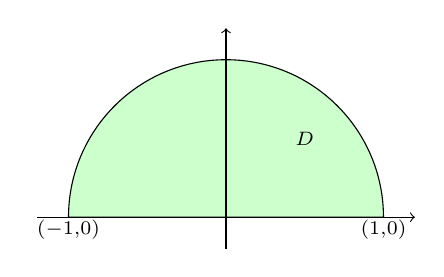
\begin{tikzpicture}[scale=2]
   \filldraw[fill=green!20,draw=black]
    (0,0) -- (1,0) arc(0:180:1) -- (0,0); 
   \draw[->] (-1.2,0) -- (1.2,0);
   \draw[->] (0,-0.2) -- (0,1.2);
   \draw(0.5,0.5) node{$\ss D$};
   \draw( 1,-0.08) node{$\ss (1,0)$}; 
   \draw(-1,-0.08) node{$\ss (-1,0)$}; 
  \end{tikzpicture}
 \end{center}
 Check the divergence theorem in this case.  (The previous exercise
 will be helpful.)
\end{exercise}
\begin{solution}
 First, we have
 \[ \dv(\vu) = \ddx(0) + \ddy(x^4+x^2y^2-x^2) = 2x^2y. \]
 We will evaluate $\iint_D\dv(\vu)\,dA$ using polar coordinates.  This
 means that $\dv(\vu)=2x^2y$ becomes $2r^3\cos^2(\tht)\sin(\tht)$, whereas
 $dA=r\,dr\,d\tht$.  The limits for $D$ are $0\leq r\leq 1$ and
 $0\leq\tht\leq\pi$ (not $2\pi$, because $D$ lies above the
 $x$-axis).  This gives
 \begin{align*}
  \iint_D\dv(\vu)\,dA 
   &= \int_{\tht=0}^{\pi}\int_{r=0}^1 2r^3\cos^2(\tht)\sin(\tht)\,r\,dr\,d\tht 
    = 2 \left(\int_{r=0}^1 r^4\,dr\right)
       \left(\int_{\tht=0}^{2\pi}\cos^2(\tht)\sin(\tht)\,d\tht\right)
 \end{align*}
 The first integral is just $\CH{r^5/5}_{r=0}^1=1/5$.  The second can
 be evaluated using the previous question:
 \begin{align*}
  \int_{\tht=0}^{\pi}\cos^2(\tht)\sin(\tht)\,d\tht &= 
   \frac{1}{4}\int_{\tht=0}^{\pi}\sin(3\tht)+\sin(\tht)\,d\tht \\
   &= \frac{1}{4}\CH{-\cos(3\tht)/3-\cos(\tht)}_{\tht=0}^\pi
    = \frac{1}{4}\left((1/3+1)-(-1/3-1)\right) \\
   &= 2/3.
 \end{align*}
 Putting this together, we get 
 \[ \iint_D\dv(\vu)\,dA  = 2 \tm \frac{1}{5} \tm \frac{2}{3}
      = \frac{4}{15}.
 \]
 On the other hand, the boundary curve can be divided into a circular
 section $C_1$ and a straight line $C_2$:
 \begin{center}
  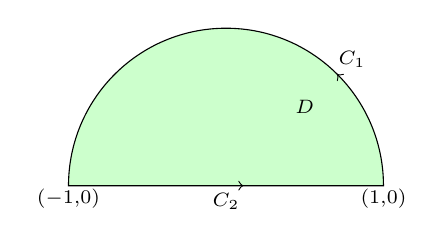
\begin{tikzpicture}[scale=2]
   \filldraw[fill=green!20,draw=black]
    (0,0) -- (1,0) arc(0:180:1) -- (0,0); 
   \draw(0.5,0.5) node{$\ss D$};
   \draw( 1,-0.08) node{$\ss (1,0)$}; 
   \draw(-1,-0.08) node{$\ss (-1,0)$}; 
   \draw(0.8,0.8) node{$\ss C_1$};
   \draw[->] (0.707,0.707) -- (0.706,0.708);
   \draw[->] (0.1,0) -- (0.11,0);
   \draw(0,-0.1) node{$\ss C_2$};
  \end{tikzpicture}
 \end{center}
 We can parametrise $C_1$ as $(x,y)=(\cos(t),\sin(t))$ for
 $0\leq t\leq\pi$.  On $C_1$ we then have
 \[ \vu = (0,x^4+x^2y^2-x^2) 
        = (0,\cos^4(t)+\cos^2(t)\sin^2(t)-\cos^2(t)).
 \]
 If we rewrite $\sin^2(t)$ as $1-\cos^2(t)$ then everything cancels
 out and we get $\vu=(0,0)$ on $C_1$, so $\int_{C_1}\vu.d\vn=0$.  On
 the other hand, we can parametrise $C_2$ as $(x,y)=(t,0)$ for
 $-1\leq t\leq 1$.  On $C_2$ we then have 
 \[ \vu = (0,x^4+x^2y^2-x^2) = (0,t^4-t^2). \]
 We also have $dx=dt$ and $dy=0$ so $d\vn=(dy,-dx)=(0,-dt)$.  This
 gives 
 \begin{align*}
  \int_{C_1}\vu.d\vn &= 
   \int_{t=-1}^1 (0,t^4-t^2).(0,-dt) = 
   \int_{t=-1}^1 t^2-t^4\,dt = 
   \CH{\frac{t^3}{3}-\frac{t^5}{5}}_{t=-1}^1 = 
   \frac{2}{3} - \frac{2}{5} = \frac{4}{15}.
 \end{align*}
 Putting this together, we get 
 \[ \int_{C}\vu.d\vn = \int_{C_1}\vu.d\vn + \int_{C_2}\vu.d\vn =
       0 + 4/15 = 4/15,
 \]
 which is the same as $\iint_D\dv(\vu)\,dA$, as expected.
\end{solution}

\begin{exercise}
 The following picture shows a hypocycloid curve $C$, which can be
 parametrised as
 \[ (x,y) = (5\cos(t)+\cos(5t),\;5\sin(t)-\sin(5t)). \]
 \begin{center}
  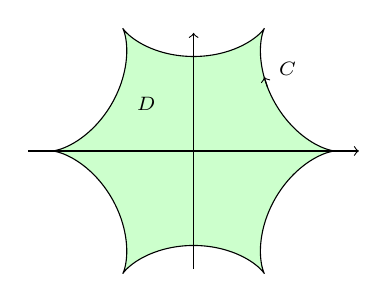
\begin{tikzpicture}[scale=0.3]
   \filldraw[fill=green!20,draw=black,domain=0:360,samples=300,smooth,variable=\t]
    plot({5*cos(\t)+cos(5*\t)},{5*sin(\t)-sin(5*\t)});
   \draw[->] (0,-5) -- (0,5);
   \draw[->] (-7,0) -- (7,0);
   \draw (-2,2) node{$\ss D$};
   \draw[->] (3.136685577,2.682092359) -- (2.986289316,3.134127162);
   \draw (3.2,2.8) node[anchor=south west] {$\ss C$};
  \end{tikzpicture}
 \end{center}
 Use the divergence theorem to find the area of the region $D$
 enclosed by $C$.  It may help to recall the identity
 \[ \cos(\al)\cos(\bt) = \half\cos(\bt+\al) + \half\cos(\bt-\al). \]
\end{exercise}
\begin{solution}
 We use same the method as was used for the deltoid in the notes and
 lectures.  We put $\vu=(x,0)$, so $\dv(\vu)=1$ and
 $\iint_D\dv(\vu)\,dA=\text{area}(D)$.  On the other hand, the
 divergence theorem tells us that this is the same as
 $\int_C\vu.d\vn$.  Using the given parametrisation of $C$ we have 
 \[ d\vn = (dy,-dx) = 
     (5\cos(t)-5\cos(5t),\;-5\sin(t)-5\sin(5t))\;dt.
 \]
 Moreover, on $C$ we have $\vu=(x,0)=(5\cos(t)+\cos(5t),0)$.  This
 gives 
 \begin{align*}
  \vu.d\vn &= (5\cos(t)+\cos(5t))(5\cos(t)-5\cos(5t)) \\
   &= 25\cos^2(t)-20\cos(t)\cos(5t)-5\cos^2(5t).
 \end{align*}
 We now use the identities
 \begin{align*}
  \cos^2(t) &= \half(1+\cos(2t)) \\
  \cos^2(5t) &= \half(1+\cos(10t)) \\
  \cos(t)\cos(5t) &= \half(\cos(6t)+\cos(4t))
 \end{align*}
 to get 
 \[ \vu.d\vn =
     \frac{25}{2} + \frac{25}{2}\cos(2t) - 
     10\cos(6t) - 10 \cos(4t) - \frac{5}{2} 
     - \frac{5}{2}\cos(10t).
 \]
 We now integrate this from $t=0$ to $t=2\pi$.  It is standard that
 $\int_{t=0}^{2\pi}\cos(kt)\,dt=0$ for any $k>0$, so most of the terms
 do not contribute anything, and we are left with 
 \[ \int_C\vu.d\vn = \int_{t=0}^{2\pi} \frac{25}{2} - \frac{5}{2}\, dt
      = \int_{t=0}^{2\pi} 10\,dt = 20\pi.
 \]
 Thus, the area of $D$ is $20\pi$. 
\end{solution}

\begin{exercise}
 Consider the following region $D$, and the vector field
 $\vu=(-y^2,x^2)$.  Verify Green's theorem for this case.
 \begin{center}
  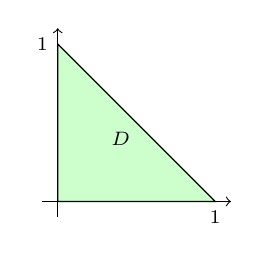
\begin{tikzpicture}[scale=2]
   \filldraw[fill=green!20,draw=black] (0,0) -- (1,0) -- (0,1) -- (0,0);
   \draw[->] (-0.1,0) -- (1.1,0);
   \draw[->] (0,-0.1) -- (0,1.1);
   \draw(0.4,0.4) node{$\ss D$};
   \draw(1,0) node[anchor=north] {$\ss 1$};
   \draw(0,1) node[anchor=east] {$\ss 1$};
  \end{tikzpicture}
 \end{center}
\end{exercise}
\begin{solution}
 First, we have 
 \[ \curl(\vu) = 
     \det\bbm \ddx & \ddy \\ -y^2 & x^2 \ebm = 
     \ddx(x^2) - \ddy(y^2) = 2x+2y.
 \]
 We now need to evaluate $\iint_D\curl(\vu)\,dA$.  The overall limits
 of $x$ in the region are $0\leq x\leq 1$.  For a fixed value of $x$
 (corresponding to a vertical strip as shown), the limits are from
 $y=0$ (at the bottom) to $y=1-x$ (at the top).
 \begin{center}
  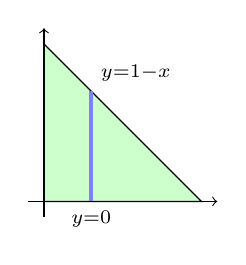
\begin{tikzpicture}[scale=2]
   \filldraw[fill=green!20,draw=black] (0,0) -- (1,0) -- (0,1) -- (0,0);
   \draw[->] (-0.1,0) -- (1.1,0);
   \draw[->] (0,-0.1) -- (0,1.1);
   \draw[ultra thick,blue!50] (0.3,0) -- (0.3,0.7);
   \draw(0.3,0.7) node[anchor=south west]{$\ss y=1-x$};
   \draw(0.3,0) node[anchor=north]{$\ss y=0$};
  \end{tikzpicture}
 \end{center}
 We thus have
 \[ \iint_D\curl(\vu)\,dA =
     \int_{x=0}^1\int_{y=0}^{1-x} 2x+2y\,dy\,dx.
 \]
 The inner integral is
 \[ \int_{y=0}^{1-x} 2x+2y \,dy =
     \CH{2xy+y^2}_{y=0}^{1-x} = 
      2x(1-x)+(1-x)^2 = 2x - 2x^2 + 1 - 2x + x^2 = 1-x^2. 
 \]
 The outer integral is therefore
 \[ \iint_D\curl(\vu)\,dA =
     \int_{x=0}^1 1-x^2 \,dx = 
     \CH{x-x^3/3}_{x=0}^1 = 2/3. 
 \]
 Green's theorem tells us that this is the same as $\int_C\vu.d\vr$,
 where $C$ is the boundary curve of $C$.  This can be broken into
 three pieces as follows:
 \begin{center}
  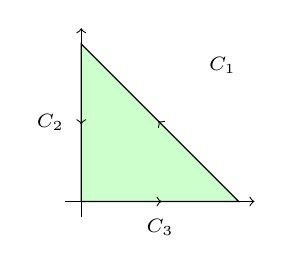
\begin{tikzpicture}[scale=2]
   \filldraw[fill=green!20,draw=black] (0,0) -- (1,0) -- (0,1) -- (0,0);
   \draw[->] (-0.1,0) -- (1.1,0);
   \draw[->] (0,-0.1) -- (0,1.1);
   \draw[->] (0.5,0.5) -- (0.49,0.51);
   \draw[->] (0.5,0) -- (0.51,0);
   \draw[->] (0,0.5) -- (0,0.49);
   \draw(0.75,0.75) node[anchor=south west] {$\ss C_1$};
   \draw(-0.05,0.5) node[anchor=east] {$\ss C_2$};
   \draw(0.5,-0.05) node[anchor=north] {$\ss C_3$};
  \end{tikzpicture}
 \end{center}
 We can parametrise $C_1$ as $(x,y)=(1-t,t)$ for $0\leq t\leq 1$.
 This gives $d\vr=(dx,dy)=(-dt,dt)$ and $\vu=(-y^2,x^2)=(-t^2,t^2)$,
 so $\vu.d\vr=2t^2\,dt$.  It follows that
 \[ \int_{C_1} \vu.d\vr = \int_{t=0}^1 2t^2\,dt =
     \CH{\frac{2}{3}t^3}_{t=0}^1 = \frac{2}{3}.
 \] 
 Next, we can parametrise $C_2$ as $(x,y)=(0,1-t)$ so
 $\vu=(-y^2,x^2=(-(1-t)^2,0)$ and $d\vr=(dx,dy)=(0,-dt)$.  This gives
 $\vu.d\vr=0$ and so $\int_{C_2}\vu.d\vr=0$.  Similarly, we can
 parametrise $C_3$ as $(x,y)=(t,0)$ giving $\vu=(0,t^2)$ and
 $d\vr=(dt,0)$ so $\vu.d\vr=0$ and $\int_{C_3}\vu.d\vr=0$.  Putting
 this together, we get 
 \[ \int_C\vu.d\vr =
     \int_{C_1}\vu.d\vr + \int_{C_2}\vu.d\vr + \int_{C_3}\vu.d\vr =
      2/3 + 0 + 0 = 2/3.
 \]
 As expected, this is the same as $\iint_D\curl(\vu)\,dA$.
\end{solution}

\begin{exercise}
 Let $f$ be any well-behaved function of two variables, and let $C$ be
 the curve where $f(x,y)=1$.  Suppose that this is a finite, closed
 curve like a circle, not branching or extending to infinity.  Explain
 three different reasons why $\int_C\grad(f).d\vr=0$.
\end{exercise}
\begin{solution}
 The most basic reason is just the fundamental theorem of calculus for
 path integrals, which says that the integral along $C$ of
 $\grad(f).d\vr$ is the change in $f$ from the beginning of $C$ to the
 end.  Here we are assuming that $C$ is a closed curve like a circle,
 so the end is the same as the beginning, so there is no change in $f$
 and $\int_C\grad(f).d\vr=0$.  Note that we do not even need the fact
 that $C$ is given by $f(x,y)=1$ here.

 Next, we can recall that $\grad(f)$ points in the direction of
 fastest possible increase of $f$, and is perpendicular to the curves
 where $f$ is constant.  As we move around $C$ the vector $d\vr$ will
 point along $C$ so $\grad(f)$ will be perpendicular to $d\vr$ and
 $\grad(f).d\vr=0$, so $\int_C\grad(f).d\vr=0$ again.

 Finally, we can use Green's theorem, which says that
 $\int_C\grad(f).d\vr=\iint_D\curl(\grad(f))\,dA$, where $D$ is the
 region enclosed by $C$.  However, we have the standard identity
 \[ \curl(\grad(f)) = \curl(f_x,f_y) = f_{yx}-f_{xy} = 0, \]
 so this integral over $D$ is again zero.
\end{solution}

\section*{Week 10 --- Surface integrals and the divergence theorem}

\begin{exercise}
 Show that
 \begin{align*}
   \sin(\al)\cos^2(\al) &= \tfrac{1}{4}(\sin(3\al)+\sin(\al)) \\
   \cos^3(\al) &= \tfrac{1}{4}\cos(3\al)+\tfrac{3}{4}\cos(\al).
 \end{align*}
 (You will need these identities in the questions below.)
\end{exercise}
\begin{solution}
 We just expand everything out using the identities
 $\cos(\al)=(e^{j\al}+e^{-j\al})/2$ and
 $\sin(\al)=(e^{j\al}-e^{-j\al})/(2j)$.  We get 
 \begin{align*}
  \sin(\al)\cos^2(\al) 
   &= \tfrac{1}{8j}(e^{j\al}-e^{-j\al})(e^{j\al}+e^{-j\al})^2 \\
   &= \tfrac{1}{8j}(e^{j\al}-e^{-j\al})(e^{2j\al}+2+e^{-2j\al}) \\
   &= \tfrac{1}{8j}(e^{3j\al}+2e^{j\al}+e^{-j\al}
                   -e^{j\al}-2e^{-j\al}-e^{-3j\al}) \\
   &= \tfrac{1}{8j}(e^{3j\al}-e^{-3j\al}+e^{j\al}-e^{-j\al}) \\
   &= \tfrac{1}{4}\left(\frac{e^{3j\al}-e^{-3j\al}}{2j}+
                        \frac{e^{j\al}-e^{-j\al}}{2j}\right) \\
   &= \tfrac{1}{4}(\sin(3\al)+\sin(\al)) \\
  \cos^3(\al)
   &= \tfrac{1}{8}(e^{j\al}+e^{-j\al})^3 \\
   &= \tfrac{1}{8}(e^{3j\al} + 3 e^{2j\al}e^{-j\al}
                    + 3 e^{j\al}e^{-2j\al} + e^{-3j\al}) \\
   &= \tfrac{1}{8}(e^{3j\al}+e^{-3j\al}+3e^{j\al}+3e^{-j\al}) \\
   &= \tfrac{1}{4}\left(\frac{e^{3j\al}+e^{-3j\al}}{2} +
                        \frac{e^{j\al}+e^{-j\al}}{2}\right)
 \end{align*}
\end{solution}

\begin{exercise}
 Evaluate $\iint_S\vF.d\vA$, where $\vF=x^2\vi+y^3\vj+z^4\vk$ and $S$
 is the surface of the cube bounded by the planes $x=0$, $x=1$, $y=0$,
 $y=1$, $z=0$ and $z=1$.
\end{exercise}
\begin{solution}
 We need to consider the six faces of the cube separately.  Let $S_1$
 be the face where $x=0$, and let $S_2$ be the face where $x=1$; in
 both cases $y$ and $z$ vary from $0$ to $1$.  On $S_1$ the outward
 unit normal vector $\vn$ is $-\vi$, but on $S_2$ we have $\vn=+\vi$.
 On $S_1$ we therefore have
 \[ \vF.\vn=-\vi.(x^2\vi+y^3\vj+z^4\vk) = -x^2, \]
 but $x=0$ on $S_1$ so $\vF.\vn=0$, so
 \[ \int_{S_1} \vF.d\vA = \int_{S_1} \vF.\vn dA = \int_{S_1} 0 dA=0.
 \]
 Similarly, on $S_2$ we have $x=1$ and $\vn=\vi$ so
 $\vF.d\vA=\vF.\vn dA=x^2\,dA=dA$, which means that
 \[ \int_{S_2} \vF.d\vA = \int_{S_2} dA = 
     \text{ area of } S_2 = 1.
 \]
 The other faces work in essentially the same way.  We have the
 following table:
 \[ \renewcommand{\arraystretch}{1.3}
    \begin{array}{|c|c|r|c|c|} \hline
     \text{face} & \text{equation} & \vn & \vF.\vn & \int \vF.d\vA \\ \hline
     S_1 & x=0 & -\vi & 0 & 0 \\ \hline
     S_2 & x=1 &  \vi & 1 & 1 \\ \hline
     S_3 & y=0 & -\vj & 0 & 0 \\ \hline
     S_4 & y=1 &  \vj & 1 & 1 \\ \hline
     S_5 & z=0 & -\vk & 0 & 0 \\ \hline
     S_6 & z=1 &  \vk & 1 & 1 \\ \hline
    \end{array}
 \]
 By adding the numbers in the last column we get $\int_S\vF.d\vA=3$. 
\end{solution}

\begin{exercise}
 Evaluate $\iint_S z^2\,dA$, where $S$ is the hemispherical shell
 given by $x^2+y^2+z^2=a^2$ with $z\geq 0$.
\end{exercise}
\begin{solution}
 This surface is given in terms of the spherical coordinates $\zen$
 and $\azi$ by 
 \[ \vr = (x,y,z) =
     (a\sin(\zen)\cos(\azi),\;a\sin(\zen)\sin(\azi),\;a\cos(\zen))
 \]
 with $0\leq\zen\leq\pi/2$ (because $\zen=\pi/2$ on the $xy$-plane)
 and $0\leq\azi\leq 2\pi$.
 This gives 
 \begin{align*}
  d\vA =& \vr_\zen\tm\vr_\azi\;d\zen\,d\azi\\
   =&
   (a\cos(\zen)\cos(\azi),\;a\cos(\zen)\sin(\azi),\;-a\sin(\zen))\tm\\
   & (-a\sin(\zen)\sin(\azi),\;a\sin(\zen)\cos(\azi),\;0)\;d\zen\,d\azi \\
   =& (a^2\sin^2(\zen)\cos(\azi),
       a^2\sin^2(\zen)\sin(\azi),
       a^2\sin(\zen)\cos(\zen)(\cos^2(\azi)+\sin^2(\azi)))\;d\zen\,d\azi \\
   =&  (a^2\sin^2(\zen)\cos(\azi),
       a^2\sin^2(\zen)\sin(\azi),
       a^2\sin(\zen)\cos(\zen))\;d\zen\,d\azi \\
   =& a^2\sin(\zen) \;
       (\sin(\zen)\cos(\azi),\;\sin(\zen)\sin(\azi),\;\cos(\zen))\;d\zen\,d\azi \\
   =& a^2\sin(\zen)\ve_r\;d\zen\,d\azi \\
   dA =& |d\vA| = a^2\sin(\zen)\;d\zen\,d\azi \\
   z^2\,dA =& (a\cos(\zen))^2\;a^2\sin(\zen)\;d\zen\,d\azi 
            = a^4\;\cos^2(\zen)\sin(\zen)\;d\zen\,d\azi.
 \end{align*}
 Using Exercise~1, this can be rewritten as 
 \begin{align*}
  z^2\,dA =& \frac{a^4}{4}(\sin(3\zen)+\sin(\zen))\;d\zen\,d\azi \\
   \int_S z^2\,dA =& \frac{a^4}{4}
    \int_{\zen=0}^{\pi/2}\int_{\azi=0}^{2\pi}
      \sin(3\zen)+\sin(\zen)\;d\azi\,d\zen \\
    =& \frac{a^4\pi}{2} \int_{\zen=0}^{\pi/2}
        \sin(3\zen)+\sin(\zen)\,d\zen \\
    =& \frac{a^4\pi}{2}
        \CH{-\tfrac{1}{3}\cos(3\zen)-\cos(\zen)}_{\zen=0}^{\pi/2} \\
    =& \frac{a^4\pi}{2}(0-(-4/3)) = 2\pi a^4/3.
 \end{align*}
\end{solution}

\begin{exercise}
 Let $S$ be the hemispherical shell given by $x^2+y^2+z^2=1$ with
 $x\geq 0$ (not $z\geq 0$).  Evaluate $\iint_S\vF.d\vA$, where
 $\vF=(1,-z,y)$.
\end{exercise}
\begin{solution}
 This surface is given in terms of the spherical coordinates $\zen$
 and $\azi$ by 
 \[ \vr = (x,y,z) =
     (\sin(\zen)\cos(\azi),\;\sin(\zen)\sin(\azi),\;\cos(\zen))
 \]
 with $-\frac{\pi}{2}\leq\azi\leq\frac{\pi}{2}$ (to ensure that
 $x\geq 0$) and $0\leq\zen\leq\pi$.  We can substitute these values
 for $x$, $y$ and $z$ into the equation $\vF=(1,\;-z,\;y)$ to get
 \[ \vF = (1,\;-\cos(\zen),\;\sin(\zen)\sin(\azi)).
 \]
 Moreover, just as in the previous exercise (with $a=1$) we have 
 \[ d\vA=\sin(\phi)\ve_r
     = (\sin^2(\zen)\cos(\azi),\;
        \sin^2(\zen)\sin(\azi),\;
        \sin(\zen)\cos(\zen))\;d\zen\,d\azi,
 \]
 so 
 \[ \vF.d\vA = \left(
     \sin^2(\zen)\cos(\azi) + 
     (-\cos(\zen))\sin^2(\zen)\sin(\azi) +
     \sin(\zen)\sin(\azi)\sin(\zen)\cos(\zen)
    \right)\;d\zen\,d\azi.
 \]
 Here the last two terms cancel, leaving 
 \[ \vF.d\vA=\sin^2(\zen)\cos(\azi)\,d\zen\,d\azi. \]
 Integrating this gives
 \begin{align*}
  \iint_S\vF.d\vA
   &= \int_{\azi=-\pi/2}^{\pi/2}\int_{\zen=0}^\pi 
       \sin^2(\zen)\cos(\azi) \,d\zen\,d\azi 
    = \int_{\azi=-\pi/2}^{\pi/2}\cos(\azi)\,d\azi 
       \int_{\zen=0}^\pi\sin^2(\zen)\,d\zen \\
   &= \CH{\sin(\azi)}_{-\frac{\pi}{2}}^{\frac{\pi}{2}} 
       \CH{\tfrac{1}{2}\zen-\tfrac{1}{4}\cos(2\zen)}_{\phi=0}^\pi \\
   &= (1-(-1))((\tfrac{\pi}{2}-\tfrac{1}{4})-(0-\tfrac{1}{4})) 
    = \pi.
 \end{align*}
\end{solution}

\begin{exercise}\ \\[-3ex]
 \begin{itemize}
  \item[(a)] Let $S$ be the cylindrical surface given parametrically
   by $x=a\cos(\azi)$ and $y=a\sin(\azi)$ with $0\leq\azi\leq 2\pi$
   and $0\leq z\leq b$.  Evaluate $\iint_S\vF.d\vA$, where
   $\vF=(x^2,y,0)$.
  \item[(b)] Now let $E$ be the solid region bounded by $S$ together
   with the planes $z=0$ and $z=b$.  Evaluate $\iiint_E\dv(\vF)dV$.
 \end{itemize}
\end{exercise}
\begin{solution}\ \\[-3ex]
 \begin{itemize}
  \item[(a)] For this surface we have
   \begin{align*}
    \vr &= (a\cos(\azi),\;a\sin(\azi),\;z) \\
    \vr_\azi &= (-a\sin(\azi),\;a\cos(\azi),\;0) \\
    \vr_z &= (0,0,1) \\
    d\vA &= (\vr_\azi\tm\vr_z)d\azi\,dz 
     = (a\cos(\azi),\;a\sin(\azi),\;0)d\azi\,dz  \\
    \vF &= (x^2,y,0) = (a^2\cos^2(\azi),\;a\sin(\azi),\;0) \\
    \vF.d\vA &= (a^3\cos^3(\azi)+a^2\sin^2(\azi))d\azi\,dz.
   \end{align*}
   This can be rewritten using Exercise~1 as 
   \[ \vF.d\vA = (\frac{a^3}{4}(\cos(3\azi)+3\cos(\azi)) +
                  \frac{a^2}{2}(1-\cos(2\azi)))d\azi\,dz.
   \]
   It is standard that 
   \[ \int_{\azi=0}^{2\pi}\cos(\azi)\,d\azi = 
      \int_{\azi=0}^{2\pi}\cos(2\azi)\,d\azi = 
      \int_{\azi=0}^{2\pi}\cos(3\azi)\,d\azi = 0.
   \]
   Using this, we find that
   \begin{align*}
    \int_S \vF.d\vA 
     &= \int_{z=0}^b \int_{\azi=0}^{2\pi}
         (\frac{a^3}{4}(\cos(3\azi)+3\cos(\azi)) +
                  \frac{a^2}{2}(1-\cos(2\azi)))d\azi\,dz \\
     &= \int_{z=0}^b \int_{\azi=0}^{2\pi}\frac{a^2}{2} d\azi\,dz \\
     &= \int_{z=0}^b a^2\pi = a^2b\pi.
   \end{align*}
  \item[(b)] First, we have
   \[ \dv(\vF) = \ddx(x^2)+\ddy(y)+\ddz(0) = 2x+1. \]
   If we work in cylindrical polar coordinates then this becomes
   $\dv(\vF)=2r\cos(\azi)+1$.  On the other hand, the volume element
   is $dV=r\,dr\,d\azi\,dz$, so 
   \begin{align*}
    \int_E\dv(\vF)\,dV 
     &= \int_{z=0}^b\int_{\azi=0}^{2\pi}\int_{r=0}^a
          (2r\cos(\azi)+1)\,r\,dr\,d\azi\,dz \\
     &= \int_{z=0}^b\int_{\azi=0}^{2\pi}\int_{r=0}^a
          (2r^2\cos(\azi)+r)\,dr\,d\azi\,dz \\
     &= \int_{z=0}^b\int_{\azi=0}^{2\pi}
         \CH{\tfrac{2}{3}r^3\cos(\azi)+\half r^2}_{r=0}^a
          d\azi\,dz \\
     &= \int_{z=0}^b\int_{\azi=0}^{2\pi}
         \tfrac{2}{3}a^3\cos(\azi)+\half a^2
          d\azi\,dz \\
     &= \int_{z=0}^b
         \CH{\tfrac{2}{3}a^3\sin(\azi)+\half a^2\azi}_{\azi=0}^{2\pi}
        \,dz \\
     &= \int_{z=0}^b a^2\pi \, dz = a^2b\pi.
   \end{align*}
 \end{itemize}
\end{solution}

\begin{exercise}
 Use the Divergence Theorem to evaluate $\iint_S\vF.d\vA$, where
 $\vF=(y^2x,z^2y,x^2z)$ and $S$ is the surface of the sphere of radius
 $a$ centred at the origin.
\end{exercise}
\begin{solution}
 First, we have
 \[ \dv(\vF) = \ddx(y^2x)+\ddy(z^2y)+\ddz(x^2z) 
     = y^2+z^2+x^2.
 \]
 If we use spherical polar coordinates, this can be written as $\dv(\vF)=r^2$.

 Now let $E$ be the unit ball enclosed by $S$.  After recalling that the
 volume element in spherical polar coordinates is
 $dV=r^2\sin(\zen)dr\,d\zen\,d\azi$, we find that
 \begin{align*}
  \iiint_E\dv(\vF)\,dV 
   &= \int_{\azi=0}^{2\pi}\int_{\zen=0}^\pi\int_{r=0}^a 
        r^4\sin(\zen)\,dr\,d\zen\,d\azi \\
   &= 2\pi \left(\int_{\zen=0}^\pi\sin(\zen)\,d\zen\right)
           \left(\int_{r=0}^a r^4\,dr\right) \\
   &= 2\pi\CH{-\cos(\zen)}_{\zen=0}^\pi\CH{\frac{r^5}{5}}_{r=0}^a
    = 2\pi\tm 2\tm \tfrac{a^5}{5} = 4\pi a^5/5.
 \end{align*}
 By the Divergence Theorem, we must have $\iint_S\vF.d\vA=4\pi a^5/5$ as well.
\end{solution}

\begin{exercise}
 Let $E$ be the solid cylinder with equations $0\leq x^2+y^2\leq a^2$
 and $0\leq z\leq b$.  Let $S$ be the surface of $E$, and let $\vF$ be
 the vector field $(x^3,y^3,z^3)$.  Use the Divergence Theorem to
 evaluate $\iint_S\vF.d\vA$.
\end{exercise}
\begin{solution}
 First, we have 
 \[ \dv(\vF) = \ddx(x^3)+\ddy(y^3)+\ddz(z^3) = 
     3(x^2+y^2+z^2).
 \]
 If we use cylindrical polar coordinates, this can be written as
 $\dv(\vF)=3r^2+3z^2$.  In those coordinates the volume element is
 $dV=r\,dr\,d\azi\,dz$, so
 \begin{align*}
  \iiint_E\dv(\vF)dV 
   &= \int_{z=0}^b \int_{\azi=0}^{2\pi} \int_{r=0}^a 
       (3r^3+3rz^2) dr\,d\azi\,dz \\
   &= \int_{z=0}^b \int_{\azi=0}^{2\pi}
       \left(\frac{3a^4}{4} + \frac{3a^2z^2}{2}\right) d\azi\,dz
    = \int_{z=0}^b (\tfrac{3}{2}\pi a^4+3\pi a^2z^2)\,dz \\
   &= \tfrac{3}{2}\pi a^4b+\pi a^2b^3 = \pi a^2b(3a^2/2+b^2).
 \end{align*}
 By the Divergence Theorem, we must have
 $\iint_S\vF.d\vA=\pi a^2b(3a^2/2+b^2)$ as well.
\end{solution}

\begin{exercise}
 Let $E$ be the cone whose top is a flat disc of radius $a$ centred on
 the $z$-axis at height $b$, and whose point is at the origin.  Let
 $S_1$ be the flat top of $E$, and let $S_2$ be the lower curved
 surface (so $S_1$ and $S_2$ together form the whole boundary of $E$).
 \begin{itemize}
  \item[(a)] Give equations for $S_1$, $S_2$ and $E$ in cylindrical
   polar coordinates.
  \item[(b)] Put $\vF=\grad(f)$, where $f=x^2+y^2+z^2$.  Show that
   $\int_{S_2}\vF.d\vA=0$, and calculate $\int_{S_1}\vF.d\vA$.
  \item[(c)] Use the Divergence Theorem to deduce the volume of $E$.
 \end{itemize}
\end{exercise}
\begin{solution}
 The picture on the left below shows the situation in three
 dimensions.  The picture on the right is a vertical cross-section.
 \begin{center}
  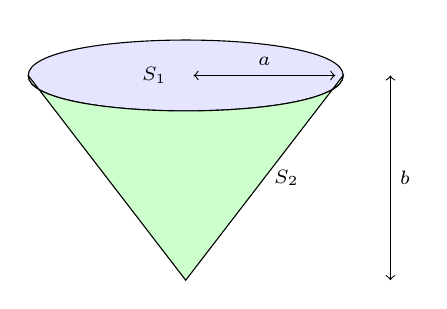
\begin{tikzpicture}[scale=2]
   \def\a{1} \def\b{1.3} \def\e{0.3} \def\d{0.23}
   \filldraw[fill=blue!10,draw=black]
    ({-\a},\b) .. controls ({-\a},{\b+\e}) and ({\a},{\b+\e}) .. ({\a},\b)
     .. controls ({\a},{\b-\e}) and ({-\a},{\b-\e}) .. ({-\a},{\b});
   \filldraw[fill=green!20,draw=black]
    ({-\a},\b) .. controls ({-\a},{\b-\e}) and ({\a},{\b-\e}) .. ({\a},\b)
    -- (0,0) -- ({-\a},\b);
   \draw(-0.2,\b) node {$\ss S_1$};
   \draw({\a/2},{\b/2}) node[anchor=west] {$\ss S_2$};
   \draw[<->] (0.05,{\b}) -- ({\a-0.05},{\b});
   \draw ({0.5*\a},{\b}) node[anchor=south] {$\ss a$};
   \draw[<->] ({1.3*\a},{\b}) -- ({1.3*\a},0);
   \draw ({1.3*\a},{0.5*\b}) node[anchor=west] {$\ss b$};
  \end{tikzpicture}
  \hspace{4em}
  \begin{tikzpicture}[scale=2]
   \draw (0,1.3) -- (1,1.3) -- (0,0) -- (0,1.5);
   \draw (0,0.65) -- (0.5,0.65);
   \draw[dotted] (0,0) -- (-1,1.3) -- (0,1.3);
   \draw[<->] (1.5,0.0) -- (1.5,1.3);
   \fill (0.00,0.00) circle(0.03);
   \fill (0.00,0.65) circle(0.03);
   \fill (0.50,0.65) circle(0.03);
   \draw (0.00,0.33) node[anchor=east] {$\ss z$}; 
   \draw (0.25,0.65) node[anchor=south] {$\ss r$}; 
   \draw (0.50,1.30) node[anchor=south] {$\ss a$};
   \draw (1.50,0.65) node[anchor=west] {$\ss b$};
   \draw (0.50,0.65) node[anchor=north west] {$\ss S_2$};
  \end{tikzpicture}
 \end{center}
 \begin{itemize}
  \item[(a)] The surface $S_1$ is given by $z=b$ with $0\leq r\leq a$
   and $0\leq\azi\leq 2\pi$.  By inspecting the right-hand picture, we
   see that the surface $S_2$ is given by $r/z=a/b$, or equivalently
   $r=az/b$, with $0\leq z\leq b$ and $0\leq\azi\leq 2\pi$.  The solid
   cylinder $E$ is given by $0\leq r\leq az/b$, again with
   $0\leq z\leq b$ and 
   $0\leq\azi\leq 2\pi$.
  \item[(b)] If $f=x^2+y^2+z^2$ and $\vF=\grad(f)$ then 
   \[ \vF=(2x,2y,2z)=(2r\cos(\azi),\;2r\sin(\azi),\;2z). \]
   In other words, $\vF$ points directly away from the origin.  This
   means that on the surface $S_1$, the vector field $\vF$ points
   along the surface, whereas $d\vA$ is perpendicular to the surface,
   so $\vF.d\vA=0$, so $\iint_{S_1}\vF.d\vA=0$.  This can be seen more 
   algebraically as follows.  On $S_2$, we have $r=az/b$, so 
   \begin{align*}
    \vr &= (az\cos(\azi)/b,az\sin(\azi)/b,z) \\
    \vF &= (2az\cos(\azi)/b,2az\sin(\azi)/b,2z) \\
    \vr_{\azi} &= (-az\sin(\azi)/b,az\cos(\azi)/b,0) \\
    \vr_z &= (a\cos(\azi)/b,\;a\sin(\azi)/b,\;1) \\
    \vF.d\vA &= \vF.(\vr_\azi\tm\vr_z) d\azi\,dz \\
     &= \det\bbm 2az\cos(\azi)/b & 2az\sin(\azi)/b & 2z \\
       -az\sin(\azi)/b & az\cos(\azi)/b & 0 \\
       a\cos(\azi)/b & a\sin(\azi)/b & 1 \ebm.
   \end{align*}
   In this matrix the top row is $2z$ times the bottom row, and it
   follows by standard properties of determinants that the determinant
   is zero.  Even more explicitly, the relevant $2\tm 2$
   subdeterminants are
   \begin{align*}
    \det\bbm  az\cos(\azi)/b & 0 \\ a\sin(\azi)/b & 1 \ebm 
     &= az\cos(\azi)/b \\
    \det\bbm -az\sin(\azi)/b & 0 \\ a\cos(\azi)/b & 1 \ebm 
     &= -az\sin(\azi)/b \\
    \det\bbm -az\sin(\azi)/b & az\cos(\azi)/b \\
             a\cos(\azi)/b & a\sin(\azi)/b \ebm 
     &= -a^2z/b^2 \\
   \end{align*}
   so the full $3\tm 3$ determinant is
   \[ 2az\cos(\azi)/b\tm az\cos(\azi)/b 
      -2az\sin(\azi)/b\tm (-az\sin(\azi)/b) + 2z\tm(-a^2z/b^2) 
       = 2a^2z^2/b^2(\cos^2(\azi)+\sin^2(\azi)-1) = 0.
   \]
   Now consider instead the surface $S_2$.  Here we have $\vn=\vk$ and
   $dA=r\,dr\,d\azi$ so $d\vA=\vn\,dA=(0,0,r)dr\,d\azi$.  We also have
   $z=b$ so 
   \begin{align*}
    \vF &= (2x,2y,2z)=(2r\cos(\azi),\;2r\sin(\azi),\;2b) \\
    \vF.d\vA &= 2br\,dr\,d\azi \\
    \iint_{S_2}\vF.d\vA
     &= \int_{\azi=0}^{2\pi}\int_{r=0}^a 2br\,dr\,d\azi 
      = \int_{\azi=0}^{2\pi}a^2b\,d\azi 
      = 2\pi a^2b.
   \end{align*}
  \item[(c)] Now note that 
   \[ \dv(\vF) = \ddx(2x)+\ddy(2y)+\ddz(2z) = 6, \]
   so 
   \[ \iiint_E\dv(\vF)\,dV = 6\tm\text{volume}(E). \]
   Using the Divergence Theorem we also see that
   \[ \iiint_E\dv(\vF)\,dV = 
       \iint_{S_1}\vF.d\vA + \iint_{S_2}\vF.d\vA = 
        0 + 2\pi a^2b = 2\pi a^2b.
   \]
   Rearranging this gives $\text{volume}(E)=(2\pi a^2b)/6=\pi a^2b/3$.
 \end{itemize}
\end{solution}

\section*{Week 11 --- Stokes's theorem}

\begin{exercise}
 Let $C$ be the vertical circle given by $y=a\sin(t)$ and $z=a\cos(t)$
 with $x=0$.  Use Stokes's Theorem to evaluate
 $\int_C(x^2y,z,0).d\vr$.  Check your answer by calculating the
 integral directly.
\end{exercise}
\begin{solution}
 Let $D$ be the vertical disc whose boundary is $C$, so $D$ can be
 parametrised by 
 \[ (x,y,z) = (0,s\sin(t),s\cos(t)) \]
 with $0\leq s\leq a$ and $0\leq t\leq 2\pi$.  We are asked to
 calculate $\int_C\vu.d\vr$, where $\vu=(x^2y,z,0)$.  Stokes's Theorem
 tells us that this is the same as $\iint_S\curl(\vu).d\vA$.  Here 
 \[ \curl(\vu)
    = \det\bbm \vi  & \vj  & \vk  \\
               \ddx & \ddy & \ddz \\
               x^2y & z    & 0 \ebm  \\
    = (-1,0,-x^2).
 \]
 It is clear that the unit normal vector to $D$ is $\vn=\pm\vi$.  By
 inspecting the diagram we see that the $\vn$ must be $-\vi$ to ensure
 that $S$ stays on the left as we walk around $C$ in the direction of
 increasing $t$.  We also have $dA=dy\,dz=s\,ds\,dt$, so 
 \begin{align*}
  \curl(\vu).d\vA &= (-1,0,-x^2).(-\vi)s\,ds\,dt = s\,ds\,dt \\
  \iint_S\curl(\vu).d\vA
   &= \int_{t=0}^{2\pi}\int_{s=0}^a s\,ds\,dt 
    = \int_{t=0}^{2\pi} \half a^2 \,dt = \pi a^2.
 \end{align*}

 Alternatively, we can calculate the line integral directly.  On $C$
 we have 
 \begin{align*}
  \vr &= (0,a\sin(t),a\cos(t)) \\
  d\vr &= (0,a\cos(t),-a\sin(t))\,dt \\
  \vu &= (x^2y,z,0) = (0,a\cos(t),0) \\
  \vu.d\vr &= a^2\cos^2(t)\,dt \\
  \int_C\vu.d\vr &= \int_{t=0}^{2\pi}a^2\cos^2(t)\,dt 
   = a^2 \int_{t=0}^{2\pi} \half(1+\cos(2t))\,dt \\
   &= a^2 \CH{\half t + \tfrac{1}{4}\sin(2t)}_{t=0}^{2\pi} = \pi a^2.
 \end{align*}
\end{solution}

\begin{exercise}
 Consider points
 \[ P = (0,0,c) \hspace{4em}
    Q = (a,0,c) \hspace{4em}
    R = (a,b,c).
 \]
 Let $C$ be the triangular path that goes from $P$ to $Q$ to $R$ and
 back to $P$.  Use Stokes's Theorem to evaluate
 $\int_C(yz^2,x^3,xy^2).d\vr$. 
\end{exercise}
\begin{solution}
 The path $C$ encloses a triangular region $S$ as shown on the left below. 
 The shadow in the $xy$-plane is shown on the right.
 \begin{center}
  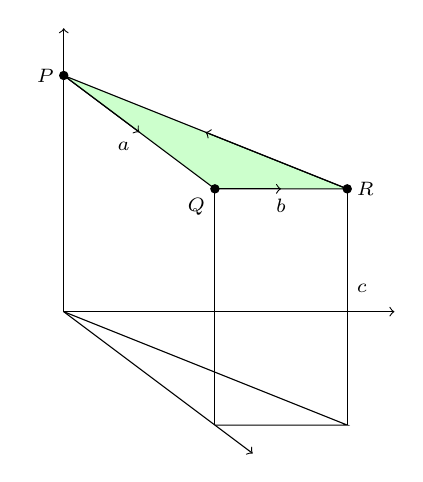
\begin{tikzpicture}[scale=3]
   \draw[->] (0,0) -- (0,1.2);
   \draw[->] (0,0) -- (1.4,0);
   \draw[->] (0,0) -- (0.8,-0.6);
   \draw (0.64,-0.48) -- (1.20,-0.48) -- (0,0);
   \draw (0.64,-0.48) -- (0.64,0.52);
   \draw (1.20,-0.48) -- (1.20,0.52);
   \filldraw[fill=green!20,draw=black] (0,1) -- (0.64,0.52) -- (1.20,0.52) -- (0,1);
   \draw[->] (0.00,1.00) -- (0.32,0.76);
   \draw[->] (0.64,0.52) -- (0.92,0.52);
   \draw[->] (1.20,0.52) -- (0.60,0.76);
   \fill (0.00,1.00) circle(0.02);
   \fill (0.64,0.52) circle(0.02);
   \fill (1.20,0.52) circle(0.02);
   \draw (0.00,1.00) node[anchor=east] {$\ss P$};
   \draw (0.64,0.52) node[anchor=north east] {$\ss Q$};
   \draw (1.20,0.52) node[anchor=west] {$\ss R$};
   \draw (0.32,0.76) node[anchor=north east] {$\ss a$};
   \draw (0.92,0.52) node[anchor=north]      {$\ss b$};
   \draw (1.20,0.10) node[anchor=west]       {$\ss c$};
  \end{tikzpicture}
  \hspace{4em}
  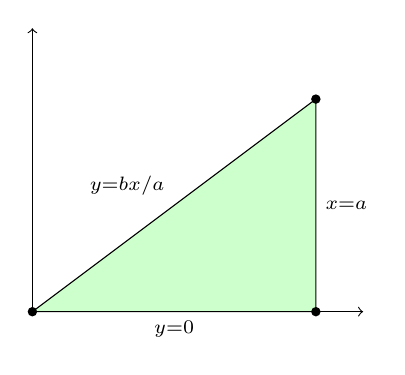
\begin{tikzpicture}[scale=3]
   \draw[->] (0,0) -- (1.4,0);
   \draw[->] (0,0) -- (0,1.2);
   \filldraw[fill=green!20,draw=black] (0,0) -- (1.2,0) -- (1.2,0.9) -- (0,0);
   \fill (0.0,0.0) circle(0.02);
   \fill (1.2,0.0) circle(0.02);
   \fill (1.2,0.9) circle(0.02);
   \draw (0.6,0.00) node[anchor=north] {$\ss y=0$};
   \draw (1.2,0.45) node[anchor=west]  {$\ss x=a$};
   \draw (0.6,0.45) node[anchor=south east] {$\ss y=bx/a$};
  \end{tikzpicture}
 \end{center}
 Consider the vector field $\vu=(yz^2,x^3,xy^2)$.  Stokes's Theorem tells us that
 $\int_C\vu.d\vr=\iint_S\curl(\vu).\vn dA$.  Here 
 \[ \curl(\vu) =
     \det \bbm \vi  & \vj  & \vk  \\
               \ddx & \ddy & \ddz \\ 
               yz^2 & x^3  & xy^2 \ebm 
     = (2xy,2yz-y^2,3x^2-z^2).
 \]
 Next, $\vn$ is clearly $(0,0,\pm 1)$.  If you walk around $C$ in the indicated
 direction with your head pointing upwards, then $S$ is on the left.  This means
 that the correct choice for $\vn$ is $(0,0,1)$, so $\curl(\vu).\vn=3x^2-z^2$, but $z=c$ 
 on $S$, so $\vu.\vn=3x^2-c^2$.  As $S$ is flat we just have
 $dA=dx\,dy$, and the right hand diagram gives us the limits, so 
 \begin{align*}
  \iint_S \curl(\vu).\vn\,dA 
   &= \int_{x=0}^a \int_{y=0}^{bx/a} 3x^2-c^2\,dy\,dx 
    = \int_{x=0}^a \CH{3x^2y-c^2y}_{y=0}^{bx/a}\,dx \\
   &= \int_{x=0}^a \tfrac{3b}{a}x^3-\tfrac{bc^2}{a}x\,dx
    = \CH{\tfrac{3b}{4a}x^4-\tfrac{bc^2}{2a}x^2}_{x=0}^a \\
   &= \tfrac{3}{4}a^3b - \tfrac{1}{2}abc^2
 \end{align*}
\end{solution}

\end{document}


\end{document}
